\chapter{Subcellular Localisation of IFIT Proteins in the Context of RSV Inclusion Bodies} \label{ch:Subcellular Localisation of IFIT Proteins in the Context of RSV Inclusion Bodies}

\section{Introduction and Aims} \label{sec:Introduction and Aims-Chapter3}
Add intro about what we think it's happening with IBs and pIBs
Using pIBs as simpler model (only N+P+ cellular components) -> h/bRSV infections -> overexpression during infection

First aim: look at how does cellular and subcellular localisation changes in response to infection, which could suggest ivolvement of IFITs with RSV lifecycle
Second aim: detaily asses the interaction of IFITs and RSV IBs during infection, with a foollow up experiments on a simplified system of pIBs, along with overexpression during infection, to further assess these


cite qupath for image analysis!!!!!!!!!!!!!


\section{Results} \label{sec:Results-Chapter3}
\subsection{IFIT Subcellular Localisation during Interferon Induction and RSV Infection} \label{subsec:IFIT Subcellular Localisation During Interferon Induction and RSV Infection}
A549, MDBK, and later BEAS2B cell lines were seeded on a 13 mm diameter glass coverslip in a 24-well plate at an initial concentration of 100,000 cells per well, as described in Section \ref{sec:Cell Culture}. 24 hours post-seeding, these cells were either mock-infected, treated with either human or bovine IFN$\upalpha$ at concentrations of 1,000 international units per mL for the former or 5 ng/mL for the latter (these concentrations are equivalent to each other), or infected with either human or bovine wild-type RSV at an MOI of 1. After 24 hours, the samples were fixed with paraformaldehyde and prepared as described in Section \ref{sec:Confocal Microscopy} for subsequent confocal microscopy analysis. The samples were stained with DAPI, allowing nuclear detection (consistently shown in yellow), antibodies against the RSV N protein (consistently shown in cyan), and the IFIT proteins (consistently shown in magenta). We initially assessed a panel of anti-IFIT antibodies, generously provided by the Viral Gene Expression Group at The Pirbright Institute. This panel included two antibodies for each of the human IFIT proteins, routinely employed for Western blotting by the group. In our confocal microscopy experiments, only one antibody per IFIT1, IFIT3, and IFIT5 yielded satisfactory results, while both antibodies against IFIT2 demonstrated efficacy. Consequently, we proceeded with single specific antibodies for IFIT1, IFIT3, and IFIT5, and utilised both IFIT2 antibodies, which we will refer to as IFIT2(A) and IFIT2(B) for simplicity.

Figure \ref{fig:Alterations in the Subcellular Localisation of Human IFITs in A549 Cells Exposed to hIFNa or hRSV} illustrates the subcellular localisation of human IFIT proteins in mock-, hIFN$\upalpha$-, or human RSV-treated samples observed in the A549 cell line. Human IFIT1 is primarily cytoplasmic and excluded from the nucleus in a basal state. Remarkably, hIFN$\upalpha$ stimulation does not alter this localisation pattern, and there is no discernible impact on the abundance of IFIT1, as evidenced by signal intensity. Throughout infection, IFIT1 maintains its cytoplasmic localisation, remaining excluded from the nucleus, potentially colocalising with N on the outer surface of the IB structure. The staining intensity exhibits an increase, particularly in uninfected cells, providing support for the hypothesis proposed in Chapter \ref{ch:Assessment of Transcriptional Induction of Human IFITs in the Context of RSV}—specifically, that RSV infection prophylactically induces IFIT expression in non-infected cells in an IFN-dependent manner. The IFIT2(A) antibody reveals hIFIT2 to be located in a cytoplasmic, diffused, but nuclearly excluded vesicular pattern in both basal and IFN$\upalpha$-induced states. The intensity between these two conditions appears equal. During hRSV infection, the overall intensity seems to decrease, and the localisation phenotype changes into a phenotype with fewer vesicles and inclusions inside the RSV IB structures. Conversely, the IFIT2(B) antibody detects IFIT2 to be granular and cytoplasmic, also depicting it as excluded from the nucleus. Similar to the IFIT2(A) antibody, the intensity and localisation phenotype between mock and IFN$\upalpha$ treated cells are equal. During hRSV infection, this antibody detects IFIT2 to be excluded from both the nucleus and the inclusion body, while retaining a vesicular cytoplasmic stain. IFIT3 appears to be cytoplasmic with nuclear exclusion under basal conditions. After IFN$\upalpha$ treatment, an increase in staining intensity and signs of IFIT3 nuclear translocation can be observed. During hRSV infection, IFIT3 seems to be evenly diffused throughout the whole cell, including the RSV inclusion body and the nucleus. The intensity of staining during infection appears similar between IFN$\upalpha$ treated and hRSV-infected cells. IFIT5 is also primarily cytoplasmically located under basal conditions while being excluded from the nucleus. During IFN$\upalpha$ treatment, the phenotype and intensity of the staining remain the same. During hRSV infection, an increase in IFIT5 levels is observed in uninfected cells. Regarding the staining pattern, it remains cytoplasmic and excluded from both the nucleus and RSV IB.

\begin{figure}
    \centering
    \includegraphics[width=1\linewidth]{08. Chapter 3/Figs/01. Localisation introduction/07. a549 merges.pdf}
    \caption[Alterations in the Subcellular Localisation of Human IFITs in A549 Cells Exposed to hIFN$\upalpha$ or hRSV.]{\textbf{Alterations in the Subcellular Localisation of Human IFITs in A549 Cells Exposed to hIFN$\upalpha$ or hRSV.} A549 cells underwent mock treatment, were treated with 1000 IU/mL of hIFN$\upalpha$ for 24 hours, or were infected with hRSV MOI 1 for 24 hours. Subsequently, cells were fixed and stained, using DAPI for nuclei detection (depicted in yellow), anti-RSV N antibody (shown in cyan), or antibodies targeting IFIT proteins (illustrated in magenta). Notably, two distinct antibodies against IFIT2 were utilised, designated as IFIT2(A) and IFIT2(B). Insets featuring magnified selections were generated from infected images, facilitating a clearer presentation of the underlying subcellular localisations.}
    \label{fig:Alterations in the Subcellular Localisation of Human IFITs in A549 Cells Exposed to hIFNa or hRSV}
\end{figure}

Figure \ref{fig:Modulations in the Subcellular Localisation of Bovine IFITs in MDBK Cells Exposed to bIFNa or bRSV} presents the subcellular localisation of bovine IFIT proteins in MDBK cell line under mock, bIFN$\upalpha$, or bovine RSV treatment conditions. Under basal conditions, bIFIT1 is primarily located in the cytoplasm with nuclear exclusion, accompanied by vesicles dispersed throughout cells, reminiscent of cytoplasmic bodies as classified by the Human Protein Atlas \cite{Thul2017AProteome}. Upon bIFN$\upalpha$ stimulation, the subcellular localisation remains unchanged, while the overall staining intensity increases. In samples infected with bRSV, cytoplasmic staining is observed with nuclear and IB exclusion, without apparent vesicles. Surrounding non-infected cells display an increased IFIT1 signal, while infected cells exhibit staining intensity lower than what was observed with interferon-stimulated cells. The IFIT2(A) antibody detects bIFIT2 predominantly in the cytoplasm, concentrated near the nucleus in a staining pattern resembling the Golgi apparatus, as classified by the Human Protein Atlas \cite{Thul2017AProteome}. This signal is also excluded from the nucleus. In interferon-treated cells, the overall pattern appears to be the same, with the exception of decreased staining intensity and decreased size of nuclearly proximal condensations. During bRSV infection, results are identical to what was observed in the A549 cell line, with the cytoplasmic signal greatly reduced. Instead, IFIT2 either colocalises with RSV N at the boundary of the IB or concentrates inside the inclusion bodies. IFIT2(B) shows bIFIT2 to be cytoplasmic with vesicles present throughout the cytoplasm and nucleus under basal conditions. It also appears to concentrate within the mitotic spindle, as classified by the Human Protein Atlas \cite{Thul2017AProteome}. Unfortunately, cells treated with bIFN$\upalpha$ and stained with IFIT2(B) antibody are lacking. During bRSV infection, this antibody shows bIFIT2 to have the same localisation and intensity as observed in mock cells. It also demonstrates IFIT2 to be excluded from the IB structure. bIFIT3 appears to be localised in vesicles with cytoplasmic and nuclear localisation in both mock and bIFN$\upalpha$ treated cells. The intensity signal appears slightly stronger in interferon-treated samples. During bRSV infection, IFIT3 subcellular localisation changes drastically. It is barely detectable in the cytoplasm and nucleus, except for strong intra-IB inclusions. There also appear to be vesicles inside the inclusion that resemble the IBAGs. bIFIT5 shows cytoplasmic localisation with vesicles diffused through the cytoplasm, weak nuclear staining, and inclusions within nucleoli. In samples treated with bIFN$\upalpha$, although the pattern of subcellular localisation remains the same, the intensity increases, especially in the nucleus. Finally, in cells infected with bRSV, nuclear exclusion occurs with inclusion within the nucleoli, and cytoplasmic staining with no clear colocalisation or exclusion with RSV IBs. The observed cytoplasmic vesicles are only evident in non-infected cells. The intensity of the staining resembles that of mock-treated cells.

\begin{figure}
    \centering
    \includegraphics[width=1\linewidth]{08. Chapter 3/Figs/01. Localisation introduction/09. mdbk-merges-test.pdf}
    \caption[Modulations in the Subcellular Localisation of Bovine IFITs in MDBK Cells Exposed to bIFN$\upalpha$ or bRSV.]{\textbf{Modulations in the Subcellular Localisation of Bovine IFITs in MDBK Cells Exposed to bIFN$\upalpha$ or bRSV.} MDBK cells underwent either mock treatment, exposure to 5 ng/mL of bIFN$\upalpha$ for 24 hours, or infection with bRSV MOI 1 for 24 hours. Subsequently, cells were fixed and stained using DAPI for nuclei detection (depicted in yellow), anti-RSV N antibody (shown in cyan), or antibodies targeting IFIT proteins (illustrated in magenta). Notably, two distinct antibodies against IFIT2 were employed, referred to as IFIT2(A) and IFIT2(B). Insets featuring magnified selections were derived from infected images, facilitating a clearer presentation of the underlying subcellular localisations.}
    \label{fig:Modulations in the Subcellular Localisation of Bovine IFITs in MDBK Cells Exposed to bIFNa or bRSV}
\end{figure}

We can observe a wide variety of subcellular localisations and interactions with the RSV inclusion bodies when these results are considered collectively. Notably, a consistent observation across cell lines and IFITs is the infrequent occurrence of changes in localisations due to IFN$\upalpha$ stimulation. Instead, it predominantly results in an increased concentration or no discernible difference compared to mock-treated samples. A noteworthy exception is the increased nuclear localisation observed in human IFIT3 and the altered pattern in bovine IFIT2, as detected by the IFIT2(A) antibody, showcasing a decreased overall signal and a modified Golgi apparatus-like staining pattern. Human and bovine IFIT1 exhibit cytoplasmic localisation with nuclear exclusion. During infection, both seem to be more expressed in uninfected cells. Bovine IFIT1, in particular, displays the presence of cytoplasmic vesicles and differential interaction with IBs, being excluded, while human IFIT1 appears to colocalise with the IB boundary. The IFIT2 antibodies provide distinct outcomes concerning the detected interaction of IFIT2 with IBs, while maintaining consistent results across human and bovine cell lines. IFIT2(A) antibody demonstrates the interaction of human and bovine IFIT2 with RSV IBs, with human IFIT2 forming intra-IB inclusions and bovine IFIT2 colocalising with the IB boundary. In contrast, IFIT2(B) consistently detects the exclusion of IFIT2 from IBs in both cell lines. Discrepancies are observed in basal localisation, both between antibodies and cell lines. In human cells, IFIT2(A) is vesicular, while IFIT2(B) exhibits a more granular cytoplasmic stain. In bovine cells, IFIT2(A) shows cytoplasmic staining with IFIT2 concentrations proximal to the nucleus, and IFIT2(B) displays a vesicular stain without these structures. Further investigation is necessary to elucidate the differential staining patterns observed with the two polyclonal antibodies. We hypothesise that these antibodies may be targeting two distinct IFIT2 epitopes. Possibilities include detection of its monomeric or dimeric state, identification of IFIT2 in complex with its interaction partners, or recognition of an unfamiliar antigenic state that requires further elucidation. Differential IFIT3 signals are noted between human and bovine cells, both in basal localisation and interaction with RSV IBs. Human IFIT3 is cytoplasmic and nuclearly excluded under basal conditions, with nuclear translocation after stimulation with either IFN$\upalpha$ or hRSV. In contrast, bovine IFIT3 is vesicular with nuclear staining under basal conditions, but nuclear staining disappears in bRSV-infected cells. Regarding RSV IB interaction, human IFIT3 is diffused evenly throughout the cytoplasm, nucleus, and IB structures, while bovine IFIT3 forms intra-IB inclusions with signs of IBAGs. Small differences are also observed between human and bovine IFIT5 staining. Both are basally cytoplasmic, with increased intensity after IFN$\upalpha$ stimulation. Bovine IFIT5 is additionally observed in cytoplasmic vesicles, nuclei, and intra-nucleolar inclusions. During infection, both human and bovine IFIT5 exhibit cytoplasmic and nuclear exclusion, with bovine IFIT5 retaining the intra-nucleolar inclusion. Regarding the interaction with RSV IBs, human IFIT5 was evidently excluded, whereas we faced challenges in definitively determining the bovine IFIT5 interaction phenotype with bovine RSV IBs.

In light of the potentially interesting findings concerning the colocalisation of IFITs with RSV IBs, we expanded our investigation with hRSV infections in the BEAS2B cell line. A comprehensive analysis was conducted, systematically examining 1727 IB sizes and their underlying interaction phenotypes with various IFIT proteins. The phenotypic categorisation was based solely on IFIT staining in regions where the presence of IBs was confirmed by viral nucleoprotein staining. Figure \ref{fig:Inclusion Bodies Within RSV Infected Cells: Zoom Sequence} illustrates a representative region of interest, showcasing its location within the cell and the broader cellular population. Based on our observations, we classified the phenotypes as follows: \textbf{Diffusion} phenotype was assigned when the IFIT signal spread equally across the area of interest; \textbf{Exclusion} phenotype was designated by an obvious, partial, or complete decrease in signal within the IB boundary; \textbf{Edge Exclusion} phenotype was assigned when the IFIT signal spread uniformly across the area of interest, except for exclusion from the IB boundary; \textbf{Inclusion} phenotype was attributed to a clear increase in the IFIT signal within the IB boundary; and \textbf{Colocalisation} phenotype was assigned when the IFIT signal spread uniformly across the area of interest, except for an increased signal in the IB boundary. Additionally, these main phenotypes were sometimes complemented by either their interaction or the presence of spots within the IB boundary. Notably, a common occurrence was colocalisation accompanied by exclusion, indicating a marked increase on the IB boundary compared to the surrounding signal, alongside a noticeable decrease within the region of interest. For the former, these spots are hypothesised to represent the inclusion body-associated granules (IBAGs). The frequency of occurrence of these phenotypes was calculated, and an arbitrary cutoff of 5\% was established to distinguish phenotypes that, due to their low frequency, were considered not relevant in the context of RSV infection.

\begin{figure}
    \centering
    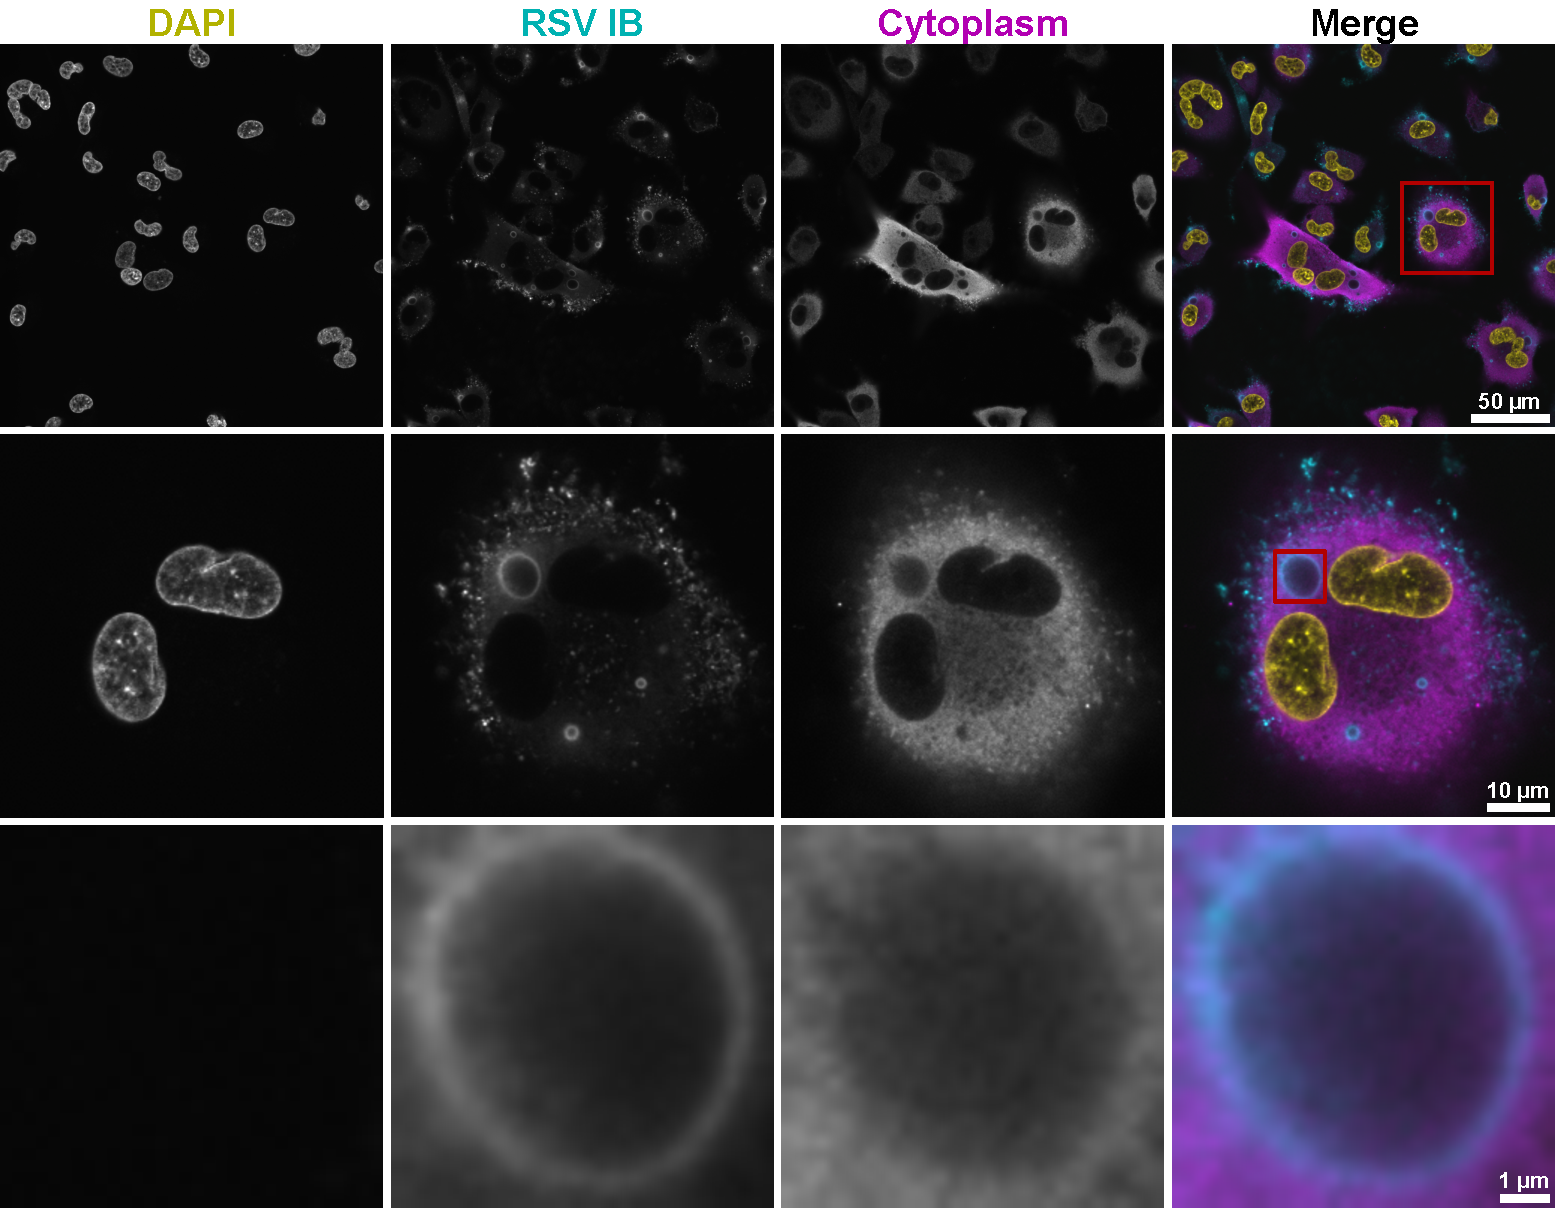
\includegraphics[width=1\linewidth]{08. Chapter 3/Figs/01. Localisation introduction/01. IB-zooms.pdf}
    \caption[Inclusion Bodies Within RSV-Infected Cells: Zoom Sequence.]{\textbf{Inclusion Bodies Within RSV-Infected Cells: Zoom Sequence.} A representative image of RSV-infected cells detected using confocal microscopy. Cellular nuclei were stained with DAPI and are depicted in yellow; RSV inclusion bodies, stained for RSV P, are represented in cyan; and the cytoplasm, stained for IFIT5, is illustrated in magenta. The figure showcases a zoom sequence starting from a population of cells, progressing to a single syncytial view, and ultimately focusing on an individual inclusion body.}
    \label{fig:Inclusion Bodies Within RSV Infected Cells: Zoom Sequence}
\end{figure}

We systematically observed and annotated a total of 1727 inclusion bodies across different cell lines, categorising their IFIT interaction phenotypes and measuring their radii (µm) and areas (\(\mbox{µm}^2\)) based on the observed 2D projections. Specifically, we analysed 1008 hRSV IBs in the A549 cell line, 99 hRSV IBs in the BEAS2B cell line, and 620 bRSV IBs in the MDBK cell line. Figure \ref{fig:Size Characterization of Inclusion Bodies Observed Across Different Cell Lines} illustrates the relationship between IB area and radius, both as an aggregate of all observed IBs and IBs detected per cell line. The data, in both the aggregate and individual cell line view, broadly follows a logarithmic curve, indicating the predominant circular shape of the majority of IBs. However, a deviation from this pattern is noticeable in each cell line, particularly in larger IBs, where the area increases disproportionately with the radius, suggesting a more elongated ellipsoid shape. Most IBs, irrespective of their origin, conform to areas below 10 \(\mbox{µm}^2\). Regarding the most common radii, both BEAS2B and MDBK IBs tend to be below 1 µm, while A549 IBs exhibit a range of the most common radii sizes between 0.5 and 1.5 µm. A more detailed view of the distribution of measured areas per cell line can be observed in Figure \ref{fig:The Distributions of IB Areas Observed Per Cell Line}. Here, all three cell lines encompass IBs ranging from sub 0.5 \(\mbox{µm}^2\) to supra 30 \(\mbox{µm}^2\), with median sizes of 5 \(\mbox{µm}^2\), 3 \(\mbox{µm}^2\), and 2 \(\mbox{µm}^2\) for A549, BEAS2B, and MDBK, respectively. MDBK has the highest number of sub 1 \(\mbox{µm}^2\) IBs, while A549 exhibits the most supra 10 \(\mbox{µm}^2\) IBs.

\begin{figure}
    \begin{subfigure}{0.495\textwidth}
        \caption{}
        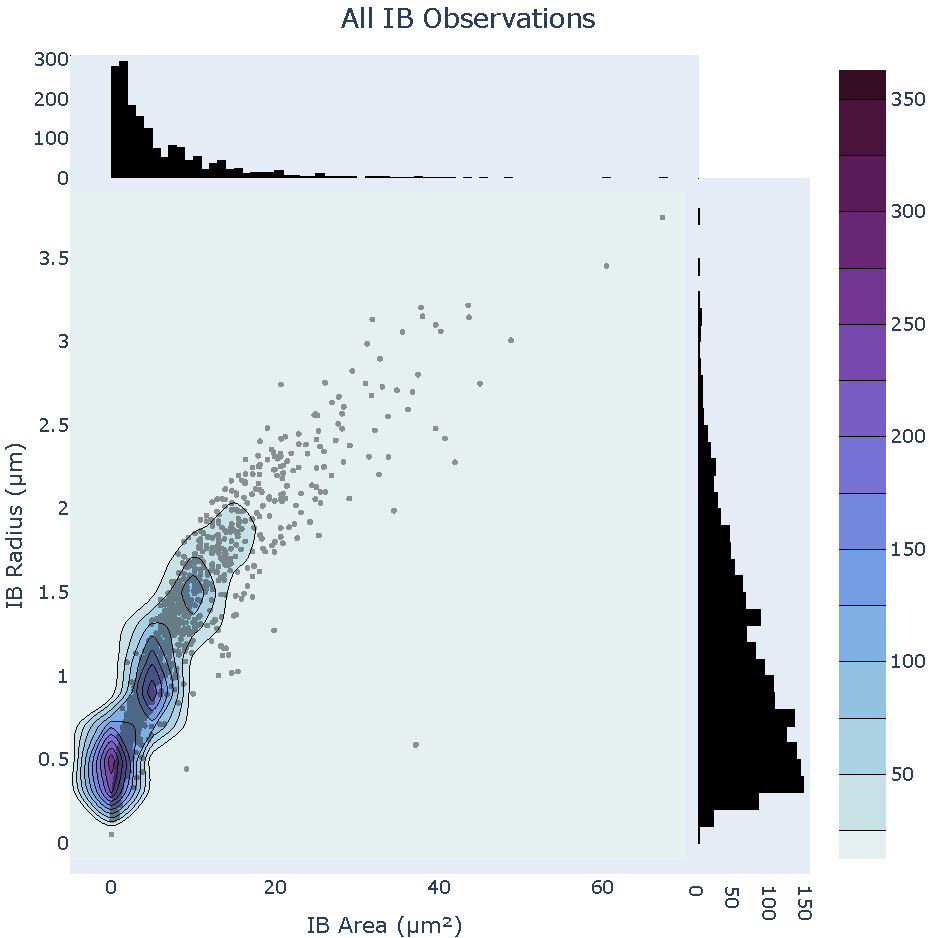
\includegraphics[width=\textwidth]{08. Chapter 3/Figs/01. Localisation introduction/02. heatmap_all.pdf} 
    \end{subfigure}
    \hfill
    \begin{subfigure}{0.495\textwidth}
        \caption{}
        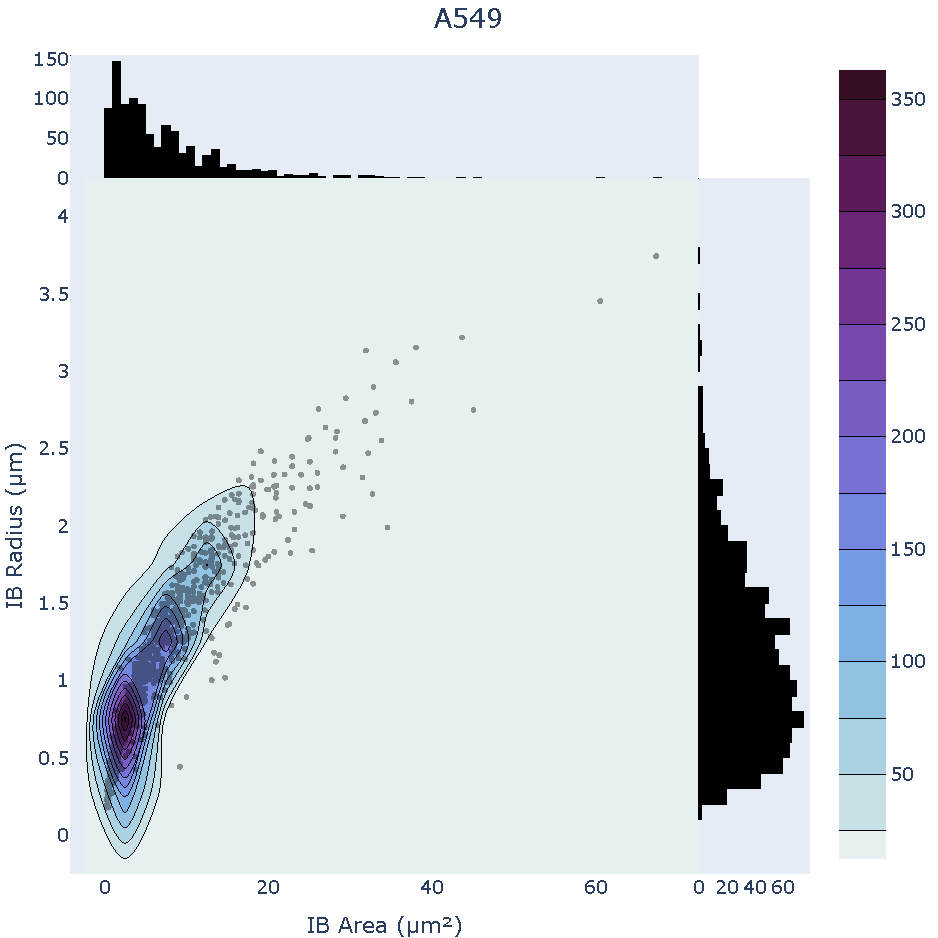
\includegraphics[width=\textwidth]{08. Chapter 3/Figs/01. Localisation introduction/03. heatmap_a549.pdf}
    \end{subfigure}

    \medskip
    \begin{subfigure}{0.495\textwidth}
        \caption{}
        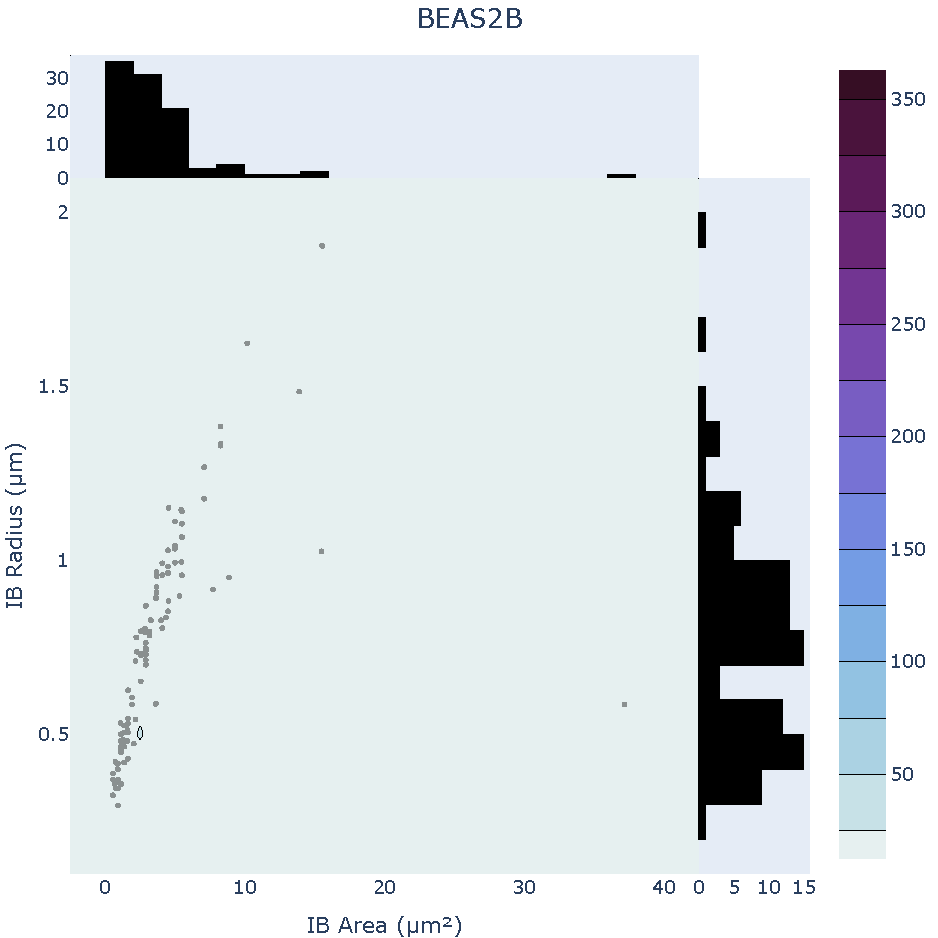
\includegraphics[width=\textwidth]{08. Chapter 3/Figs/01. Localisation introduction/04. heatmap_beas2b.pdf} 
    \end{subfigure}
    \hfill
    \begin{subfigure}{0.495\textwidth}
        \caption{}
        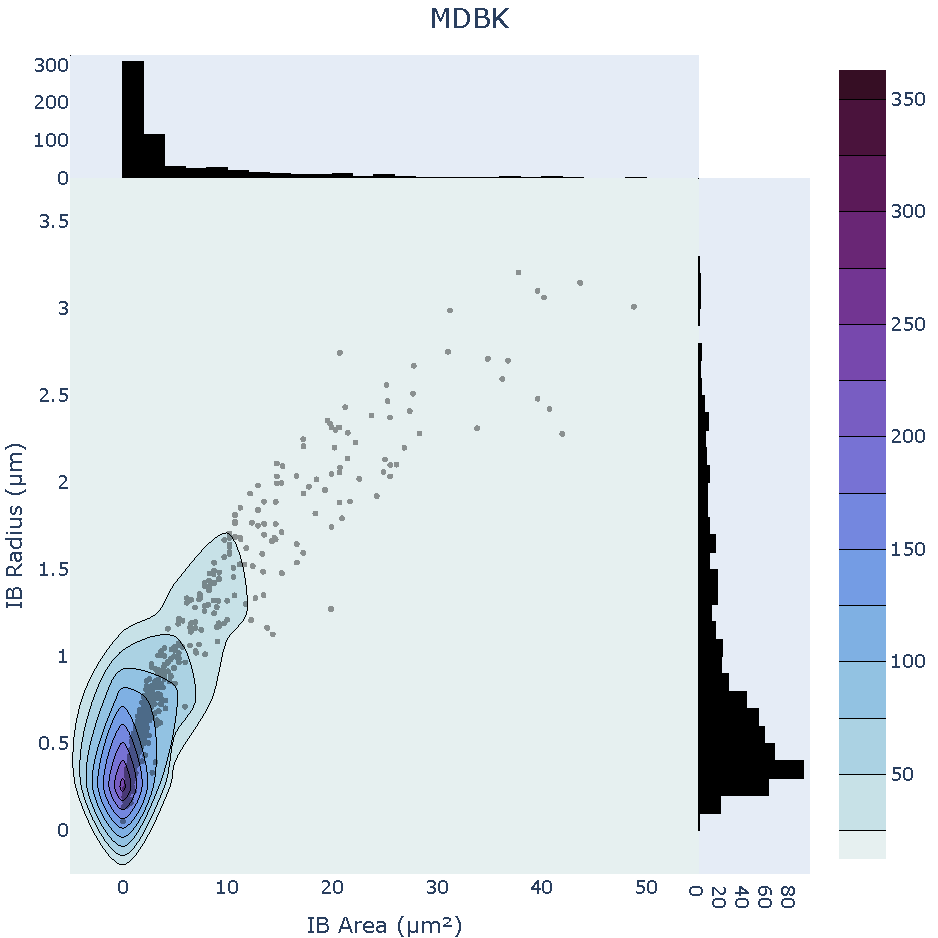
\includegraphics[width=\textwidth]{08. Chapter 3/Figs/01. Localisation introduction/05. heatmap_mdbk.pdf} 
    \end{subfigure}
    \caption[Size Characterisation of Inclusion Bodies Observed Across Different Cell Lines.]{\textbf{Size Characterisation of Inclusion Bodies Observed Across Different Cell Lines.} This figure elucidates the relationship between the measured area (\(\mbox{µm}^2\)) and radius (µm) of individual RSV inclusion bodies observed in this study. The figure includes distinct population distributions alongside the plots: (a) an aggregate of 1727 IB observations across all cell lines, (b) 1008 observations from the A549 cell line, (c) 99 observations from the BEAS2B cell line, and (d) 620 observations from the MDBK cell line. Contour plots are incorporated to highlight the density of individual IBs within the plots.}
    \label{fig:Size Characterization of Inclusion Bodies Observed Across Different Cell Lines}
\end{figure}

From the published literature, it is established that an increase in IB area correlates with its maturation state and internal complexity. Notably, in the HEp-2 cell line infected with hRSV, it has been reported that IBs containing IBAGs are significantly larger than those without (6.4 \(\mbox{µm}^2\) versus 2.3 \(\mbox{µm}^2\)) \cite{Rincheval2017FunctionalVirus}. Additionally, in the MDBK cell line, during the early infection timepoint (6 hours post-infection), only small IBs are present, with a mean area value of 1 \(\mbox{µm}^2\), and these do not contain IBAGs. At 16 hours post-infection, IBs without IBAGs retain the mean area value, while larger IBs with IBAGs (mean area of 10 \(\mbox{µm}^2\)) are also observed \cite{Jobe2021BovineResponses}. Importantly, at 24 HPI, a critical timepoint for the analysis in this thesis, small IBs without IBAGs maintain a median size of 1 \(\mbox{µm}^2\), while larger IBs containing IBAGs cluster into two sizes, with mean areas of 2.5 \(\mbox{µm}^2\) and 17 \(\mbox{µm}^2\). Based on this information, we can assess the observed IFIT-IB interaction phenotypes per mature or immature IBs.

\begin{figure}
    \centering
    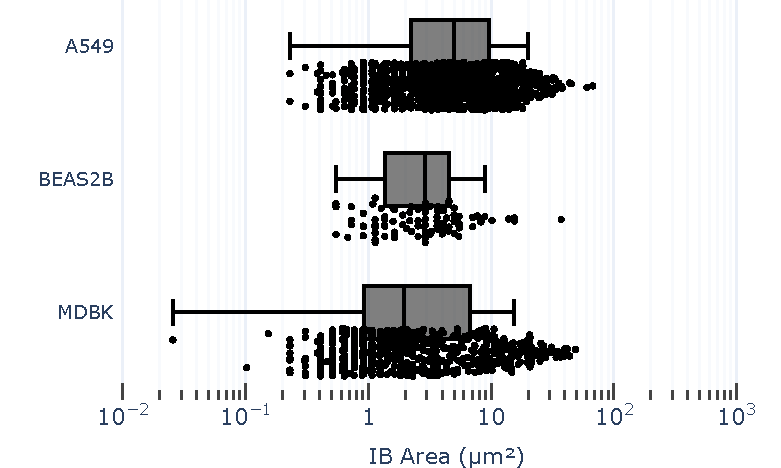
\includegraphics[width=1\linewidth]{08. Chapter 3/Figs/01. Localisation introduction/06. box-infection.pdf}
    \caption[The Distributions of IB Areas Observed per Cell Line.]{\textbf{The Distributions of IB Areas Observed per Cell Line.} The distribution of RSV inclusion body areas (\(\mbox{µm}^2\)), detected in this study are shown. A total of 1008 observations were made in the A549 cell line, 99 observations in the BEAS2B cell line, and 620 observations in the MDBK cell line.}
    \label{fig:The Distributions of IB Areas Observed Per Cell Line}
\end{figure}
\subsection{Nascent Human and Bovine IFIT Localisation During RSV Infection} \label{subsec:Nascent Human and Bovine IFIT Localisation During RSV Infection}
\subsubsection{Phenotypic Diversity of Nascent IFIT1 Interaction with RSV Inclusion Bodies}
following a hint of interaction with ibs for some ifits, we went to systematically assess the interaction of all ifits

ifit one, although being predominantly excluded or duffuesd through ibs (suggesting no interaction), is often observed to interact with these structures

inclusion and coloc + eclusion happens in larger ibs (probs more mature), suggesting temporal nature of ifit one interaction

30 excl 30 diff 18 incl 9 coloc + excl 9 edge excl
5, 4.4, 8, 12, 7

\lipsum[1-30]
\begin{figure}
    \begin{subfigure}{0.495\textwidth}
        \caption{}
        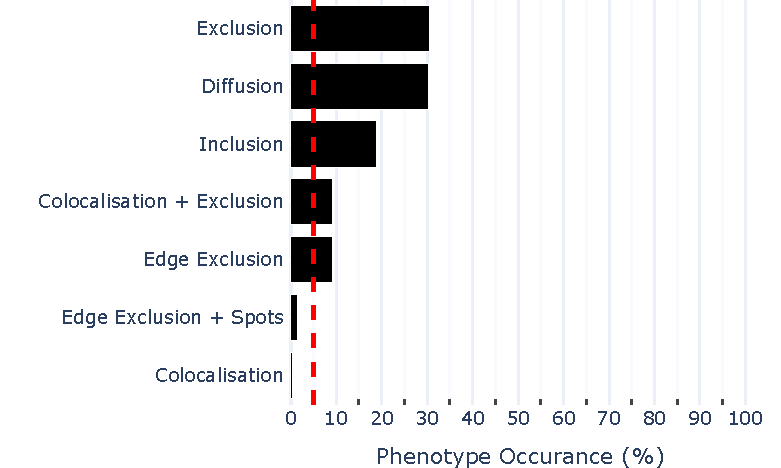
\includegraphics[width=1\linewidth]{08. Chapter 3/Figs/02. Infection/01. IFIT1/01. bar_i1_a549.pdf} 
    \end{subfigure}
    \begin{subfigure}{0.495\textwidth}
        \caption{}
        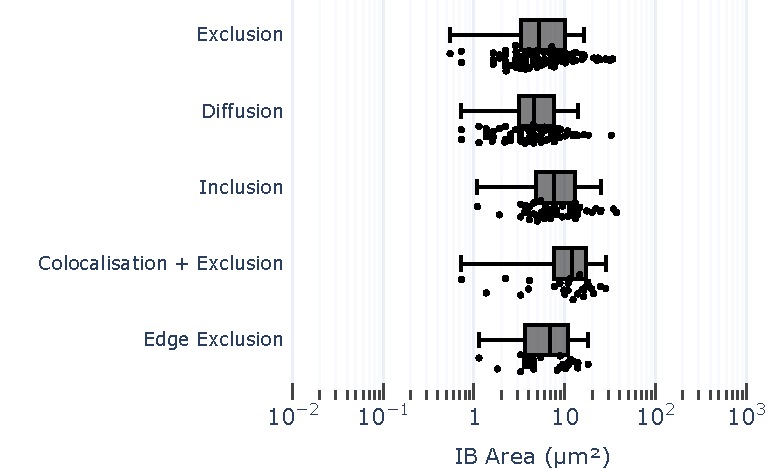
\includegraphics[width=1\linewidth]{08. Chapter 3/Figs/02. Infection/01. IFIT1/02. box_i1_a549.pdf}
    \end{subfigure}
    \caption[Phenotypic Diversity of hIFIT1 Interactions with hRSV Inclusion Bodies in A549 Cell Line.]{\textbf{Phenotypic Diversity of hIFIT1 Interactions with hRSV Inclusion Bodies in A549 Cell Line.} A549 cells were infected with human RSV at MOI 1 and fixed 24 HPI. Cells were double-labeled with with anti-RSV N and anti-IFIT1 antibodies and imaged on confocal microscope. Panel (a) shows percentual proportions of observed phenotypes between hRSV inclusion bodies and hIFIT1 (281 observations), with the red dotted line denoting the 5\% threshold, marking phenotypes considered relevant above this limit. Panel (b) shows the IB area in \(\mu m^2\) per observed relevant phenotype.}
    \label{fig:Phenotypic Diversity of hIFIT1 Interactions with hRSV Inclusion Bodies in A549 Cell Line}
\end{figure}

\begin{figure}
    \centering
    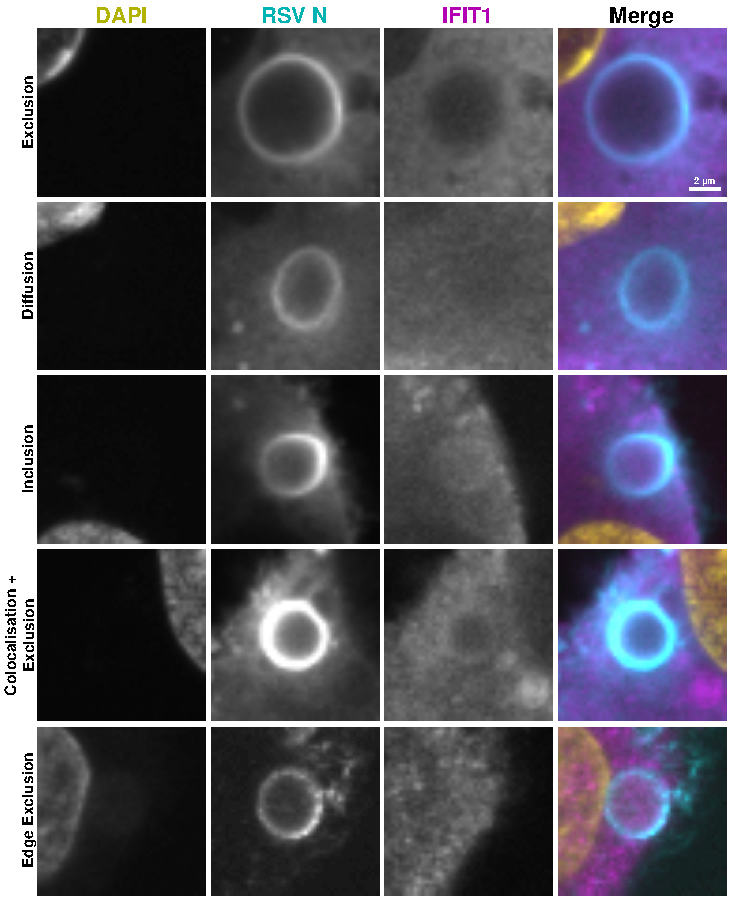
\includegraphics[width=1\linewidth]{08. Chapter 3/Figs/02. Infection/01. IFIT1/03. a549 i1.pdf}
    \caption[Representative Images of Phenotypic Diversity of hIFIT1 Interactions with hRSV Inclusion Bodies in A549 Cell Line.]{\textbf{Representative Images of Phenotypic Diversity of hIFIT1 Interactions with hRSV Inclusion Bodies in A549 Cell Line.} A549 cells were infected with hRSV at MOI 1 and fixed at 24 HPI. Cellular nuclei were stained with DAPI (yellow), and cells were double-labeled with anti-RSV N (cyan) and anti-IFIT1 (magenta) antibodies. This figure showcases representative examples of relevant phenotypes in the interaction between hIFIT1 and hRSV inclusion bodies. These phenotypes are presented in descending order based on their percentage proportions. The scale bar indicates 2 \(\mu m\).}
    \label{fig:Representative Images of Phenotypic Diversity of hIFIT1 Interactions with hRSV Inclusion Bodies in A549 Cell Line}
\end{figure}

in beas2bs there is mainly exclsion 86\% with some diffusion 8\%.

diffusion happens in smaller ibs 0.5 (compared to 3)

\begin{figure}
    \begin{subfigure}{0.495\textwidth}
        \caption{}
        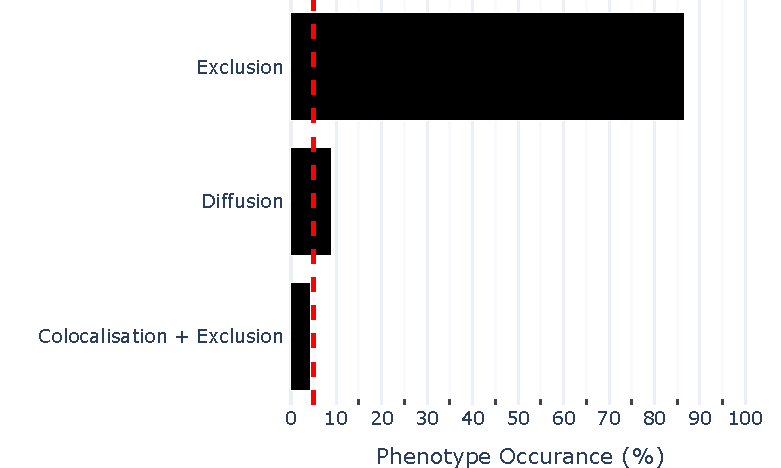
\includegraphics[width=1\linewidth]{08. Chapter 3/Figs/02. Infection/01. IFIT1/04. bar_i1_beas2b.pdf} 
    \end{subfigure}
    \begin{subfigure}{0.495\textwidth}
        \caption{}
        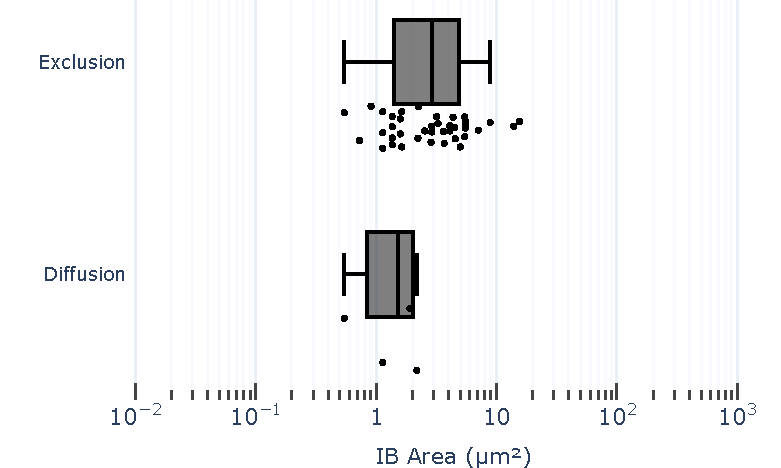
\includegraphics[width=1\linewidth]{08. Chapter 3/Figs/02. Infection/01. IFIT1/05. box_i1_beas2b.pdf}
    \end{subfigure}
    \caption[Phenotypic Diversity of hIFIT1 Interactions with hRSV Inclusion Bodies in BEAS2B Cell Line.]{\textbf{Phenotypic Diversity of hIFIT1 Interactions with hRSV Inclusion Bodies in BEAS2B Cell Line.} BEAS2B cells were infected with human RSV at MOI 1 and fixed 24 HPI. Cells were double-labeled with with anti-RSV N and anti-IFIT1 antibodies and imaged on confocal microscope. Panel (a) shows percentual proportions of observed phenotypes between hRSV inclusion bodies and hIFIT1 (281 observations), with the red dotted line denoting the 5\% threshold, marking phenotypes considered relevant above this limit. Panel (b) shows the IB area in \(\mu m^2\) per observed relevant phenotype.}
    \label{fig:Phenotypic Diversity of hIFIT1 Interactions with hRSV Inclusion Bodies in BEAS2B Cell Line}
\end{figure}

\begin{figure}
    \centering
    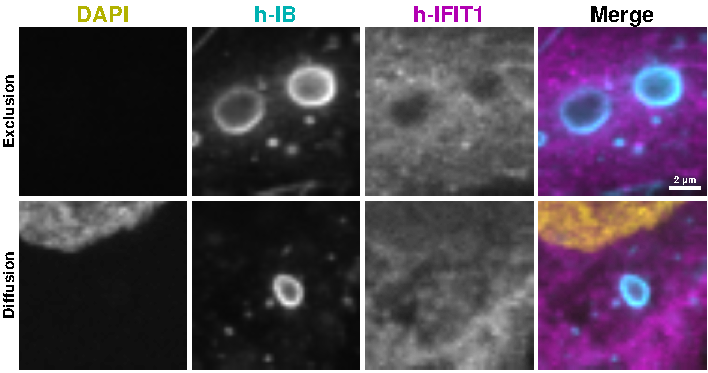
\includegraphics[width=1\linewidth]{08. Chapter 3/Figs/02. Infection/01. IFIT1/06. beas2b i1.pdf}
    \caption[Representative Images of Phenotypic Diversity of hIFIT1 Interactions with hRSV Inclusion Bodies in BEAS2B Cell Line.]{\textbf{Representative Images of Phenotypic Diversity of hIFIT1 Interactions with hRSV Inclusion Bodies in BEAS2B Cell Line.} BEAS2B cells were infected with hRSV at MOI 1 and fixed at 24 HPI. Cellular nuclei were stained with DAPI (yellow), and cells were double-labeled with anti-RSV N (cyan) and anti-IFIT1 (magenta) antibodies. This figure showcases representative examples of relevant phenotypes in the interaction between hIFIT1 and hRSV inclusion bodies. These phenotypes are presented in descending order based on their percentage proportions. The scale bar indicates 2 \(\mu m\).}
    \label{fig:Representative Images of Phenotypic Diversity of hIFIT1 Interactions with hRSV Inclusion Bodies in BEAS2B Cell Line}
\end{figure}

66 excl, 23 incl, 5 diff

2, 1, 1.5

\begin{figure}
    \begin{subfigure}{0.495\textwidth}
        \caption{}
        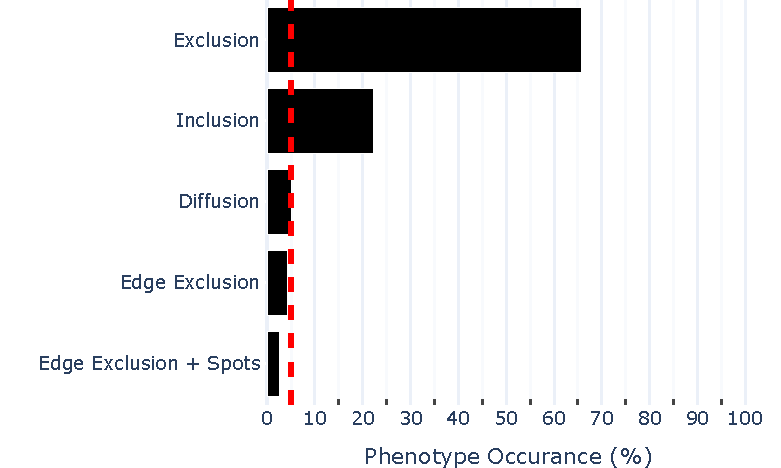
\includegraphics[width=1\linewidth]{08. Chapter 3/Figs/02. Infection/01. IFIT1/07. bar_i1_mdbk.pdf} 
    \end{subfigure}
    \begin{subfigure}{0.495\textwidth}
        \caption{}
        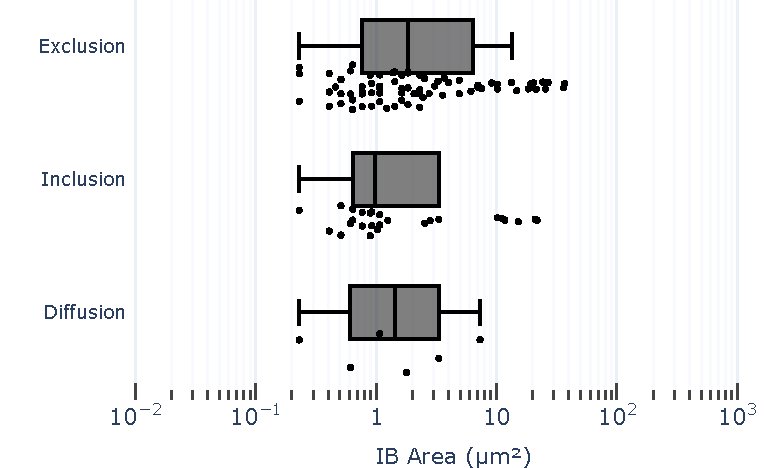
\includegraphics[width=1\linewidth]{08. Chapter 3/Figs/02. Infection/01. IFIT1/08. box_i1_mdbk.pdf}
    \end{subfigure}
    \caption[Phenotypic Diversity of bIFIT1 Interactions with bRSV Inclusion Bodies in MDBK Cell Line.]{\textbf{Phenotypic Diversity of bIFIT1 Interactions with bRSV Inclusion Bodies in MDBK Cell Line.} MDBK cells were infected with bovine RSV at MOI 1 and fixed 24 HPI. Cells were double-labeled with with anti-RSV N and anti-IFIT1 antibodies and imaged on confocal microscope. Panel (a) shows percentual proportions of observed phenotypes between bRSV inclusion bodies and bIFIT1 (117 observations), with the red dotted line denoting the 5\% threshold, marking phenotypes considered relevant above this limit. Panel (b) shows the IB area in \(\mu m^2\) per observed relevant phenotype.}
    \label{fig:Phenotypic Diversity of bIFIT1 Interactions with bRSV Inclusion Bodies in MDBK Cell Line}
\end{figure}

\begin{figure}
    \centering
    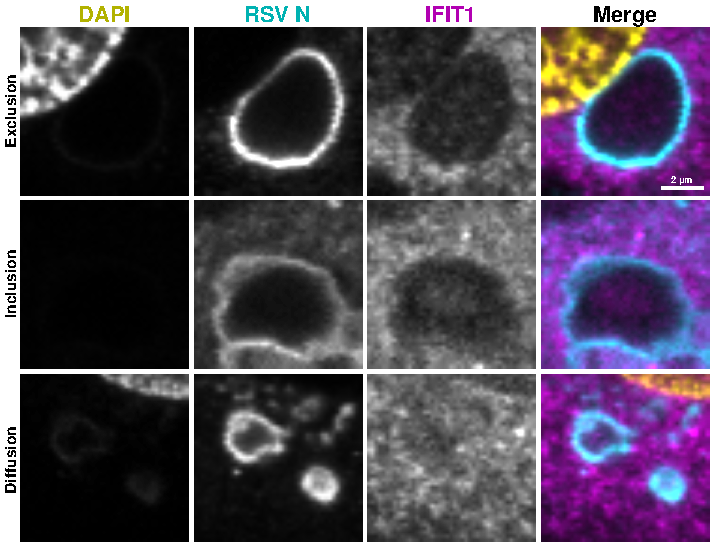
\includegraphics[width=1\linewidth]{08. Chapter 3/Figs/02. Infection/01. IFIT1/09. mdbk i1.pdf}
    \caption[Representative Images of Phenotypic Diversity of bIFIT1 Interactions with bRSV Inclusion Bodies in MDBK Cell Line.]{\textbf{Representative Images of Phenotypic Diversity of bIFIT1 Interactions with bRSV Inclusion Bodies in MDBK Cell Line.} MDBK cells were infected with bRSV at MOI 1 and fixed at 24 HPI. Cellular nuclei were stained with DAPI (yellow), and cells were double-labeled with anti-RSV N (cyan) and anti-IFIT1 (magenta) antibodies. This figure showcases representative examples of relevant phenotypes in the interaction between bIFIT1 and bRSV inclusion bodies. These phenotypes are presented in descending order based on their percentage proportions. The scale bar indicates 2 \(\mu m\).}
    \label{fig:Representative Images of Phenotypic Diversity of bIFIT1 Interactions with bRSV Inclusion Bodies in MDBK Cell Line}
\end{figure}

\subsubsection{Phenotypic Diversity of Nascent IFIT2 Interaction with RSV Inclusion Bodies}

\begin{figure}
    \begin{subfigure}{0.495\textwidth}
        \caption{}
        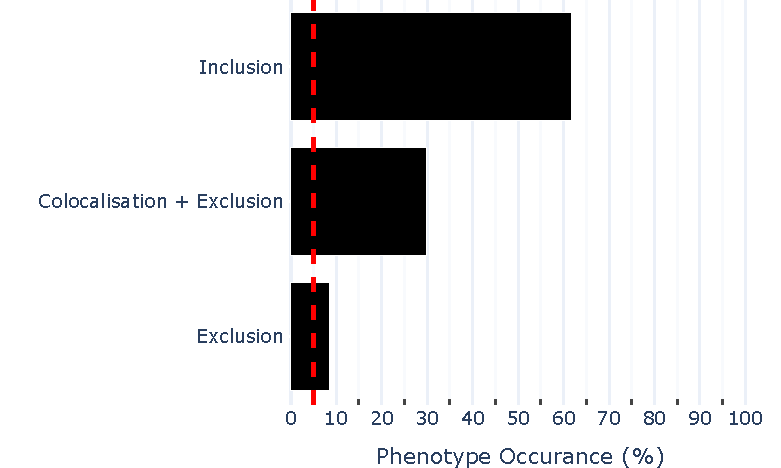
\includegraphics[width=1\linewidth]{08. Chapter 3/Figs/02. Infection/02. IFIT2/01. IFIT2A/01. bar_i2a_a549-n.pdf}
    \end{subfigure}
    \begin{subfigure}{0.495\textwidth}
        \caption{}
        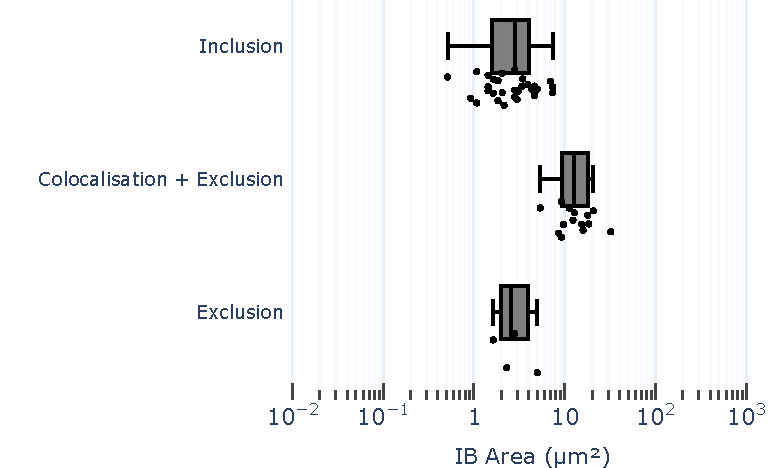
\includegraphics[width=1\linewidth]{08. Chapter 3/Figs/02. Infection/02. IFIT2/01. IFIT2A/02. box_i2a_a549-n.pdf}
    \end{subfigure}
    \caption[Phenotypic Diversity of hIFIT2 Interactions with Nucleoprotein-Stained hRSV Inclusion Bodies, Detected by IFIT2A Antibody in A549 Cell Line.]{\textbf{Phenotypic Diversity of hIFIT2 Interactions with Nucleoprotein-Stained hRSV Inclusion Bodies, Detected by IFIT2A Antibody in A549 Cell Line.} A549 cells were infected with human RSV at MOI 1 and fixed 24 HPI. Cells were labeled with anti-RSV N and anti-IFIT2A antibodies and imaged on confocal microscope. Panel (a) shows percentual proportions of observed phenotypes between hRSV inclusion bodies and hIFIT2, detected by IFIT2A antibody (47 observations), with the red dotted line denoting the 5\% threshold, marking phenotypes considered relevant above this limit. Panel (b) shows the IB area in \(\mu m^2\) per observed relevant phenotype.}
    \label{fig:Phenotypic Diversity of hIFIT2 Interactions with Nucleoprotein-Stained hRSV Inclusion Bodies, Detected by IFIT2A Antibody in A549 Cell Line}
\end{figure}

\begin{figure}
    \centering
    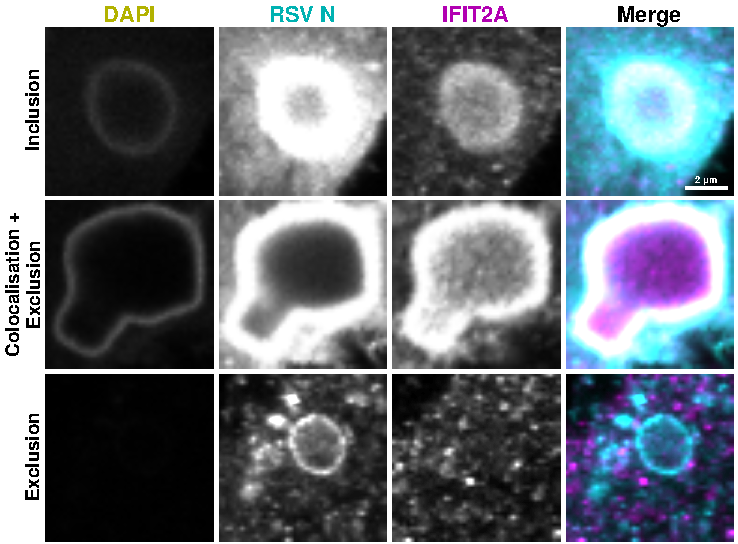
\includegraphics[width=1\linewidth]{08. Chapter 3/Figs/02. Infection/02. IFIT2/01. IFIT2A/03. i2a a549 hrsv n.pdf}
    \caption[Representative Images of Phenotypic Diversity of hIFIT2 Interactions with Nucleoprotein-Stained hRSV Inclusion Bodies, Detected by IFIT2A Antibody in A549 Cell Line.]{\textbf{Representative Images of Phenotypic Diversity of hIFIT2 Interactions with Nucleoprotein-Stained hRSV Inclusion Bodies, Detected by IFIT2A Antibody in A549 Cell Line.} A549 cells were infected with hRSV at MOI 1 and fixed at 24 HPI. Cellular nuclei were stained with DAPI (yellow), and cells were double-labeled with anti-RSV N (cyan) and anti-IFIT2A (magenta) antibodies. This figure showcases representative examples of relevant phenotypes in the interaction between hIFIT2, detected by IFIT2A antibody, and hRSV inclusion bodies. These phenotypes are presented in descending order based on their percentage proportions. The scale bar indicates 2 \(\mu m\).}
    \label{fig:Representative Images of Phenotypic Diversity of hIFIT2 Interactions with Nucleoprotein-Stained hRSV Inclusion Bodies, Detected by IFIT2A Antibody in A549 Cell Line}
\end{figure}

60 30 8

3 12 2.6

Nascent human IFIT2 colocalises with the ring structure (outlined by RSV P staining) and to the inner edge of the IB.

\begin{figure}
    \begin{subfigure}{0.495\textwidth}
        \caption{}
        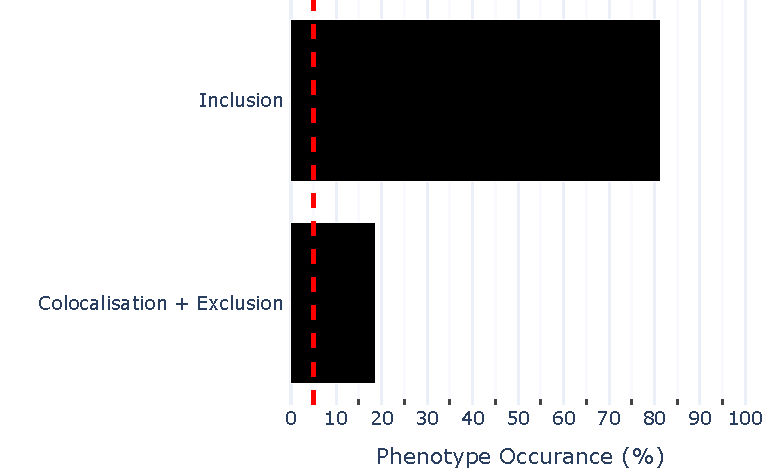
\includegraphics[width=1\linewidth]{08. Chapter 3/Figs/02. Infection/02. IFIT2/01. IFIT2A/04. bar_i2a_a549-p.pdf} 
    \end{subfigure}
    \begin{subfigure}{0.495\textwidth}
        \caption{}
        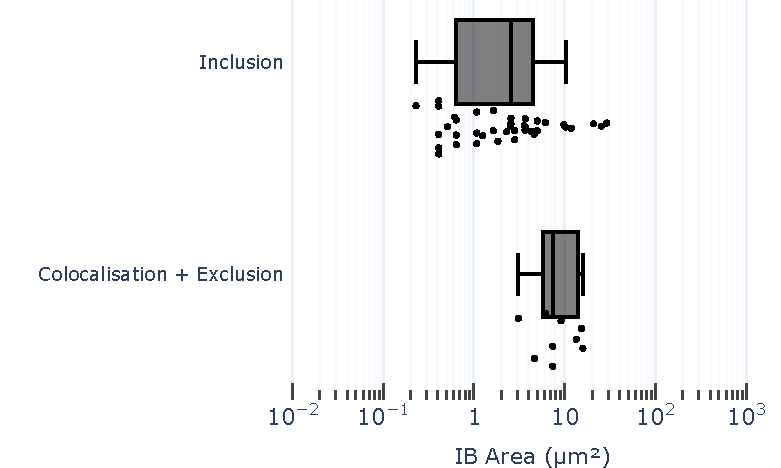
\includegraphics[width=1\linewidth]{08. Chapter 3/Figs/02. Infection/02. IFIT2/01. IFIT2A/05. box_i2a_a549-p.pdf}
    \end{subfigure}
    \caption[Phenotypic Diversity of hIFIT2 Interactions with Phosphoprotein-Stained hRSV Inclusion Bodies, Detected by IFIT2A Antibody in A549 Cell Line.]{\textbf{Phenotypic Diversity of hIFIT2 Interactions with Phosphoprotein-Stained hRSV Inclusion Bodies, Detected by IFIT2A Antibody in A549 Cell Line.} A549 cells were infected with human RSV at MOI 1 and fixed 24 HPI. Cells were labeled with anti-RSV P and anti-IFIT2A antibodies and imaged on confocal microscope. Panel (a) shows percentual proportions of observed phenotypes between hRSV inclusion bodies and hIFIT2, detected by IFIT2A antibody (48 observations), with the red dotted line denoting the 5\% threshold, marking phenotypes considered relevant above this limit. Panel (b) shows the IB area in \(\mu m^2\) per observed relevant phenotype.}
    \label{fig:Phenotypic Diversity of hIFIT2 Interactions with Phosphoprotein-Stained hRSV Inclusion Bodies, Detected by IFIT2A Antibody in A549 Cell Line}
\end{figure}

\begin{figure}
    \centering
    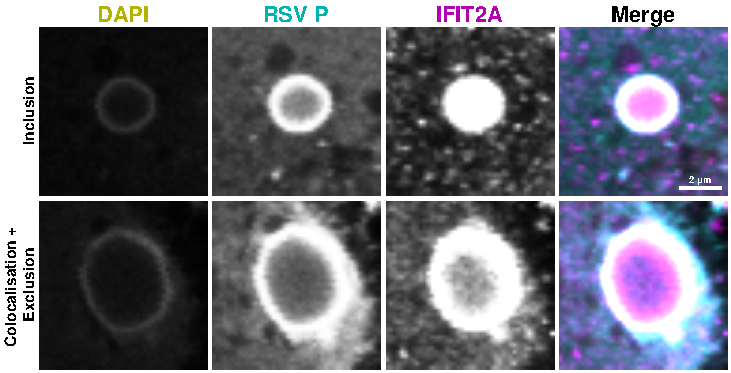
\includegraphics[width=1\linewidth]{08. Chapter 3/Figs/02. Infection/02. IFIT2/01. IFIT2A/06. i2a a549 hrsv p.pdf} 
    \caption[Representative Images of Phenotypic Diversity of hIFIT2 Interactions with Phosphoprotein-Stained hRSV Inclusion Bodies, Detected by IFIT2A Antibody in A549 Cell Line.]{\textbf{Representative Images of Phenotypic Diversity of hIFIT2 Interactions with Phosphoprotein-Stained hRSV Inclusion Bodies, Detected by IFIT2A Antibody in A549 Cell Line.} A549 cells were infected with hRSV at MOI 1 and fixed at 24 HPI. Cellular nuclei were stained with DAPI (yellow), and cells were double-labeled with anti-RSV P (cyan) and anti-IFIT2A (magenta) antibodies. This figure showcases representative examples of relevant phenotypes in the interaction between hIFIT2, detected by IFIT2A antibody, and hRSV inclusion bodies. These phenotypes are presented in descending order based on their percentage proportions. The scale bar indicates 2 \(\mu m\).}
    \label{fig:Representative Images of Phenotypic Diversity of hIFIT2 Interactions with Phosphoprotein-Stained hRSV Inclusion Bodies, Detected by IFIT2A Antibody in A549 Cell Line}
\end{figure}

82 18

2.5 7.3

With regards of colocalization with human RSV M2/1 protein, human IFIT2 seems to either form inclusion, which has a signal decrease towards the middle of the IB structure (top panel), or seems to strongly colocalise with the ring structure highlighted by M2/1 staining (bottom 2 panels; there also seems to be IFIT2 signal concentration on the inner edge of the IB structure).

\begin{figure}
    \begin{subfigure}{0.495\textwidth}
        \caption{}
        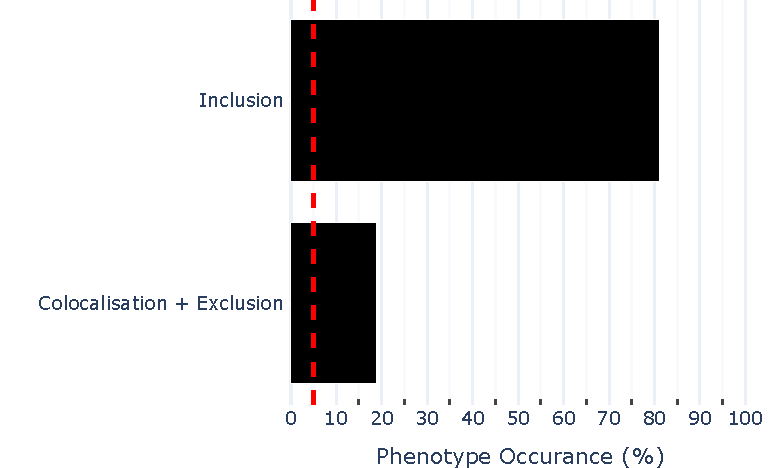
\includegraphics[width=1\linewidth]{08. Chapter 3/Figs/02. Infection/02. IFIT2/01. IFIT2A/07. bar_i2a_a549-m21.pdf} 
    \end{subfigure}
    \begin{subfigure}{0.495\textwidth}
        \caption{}
        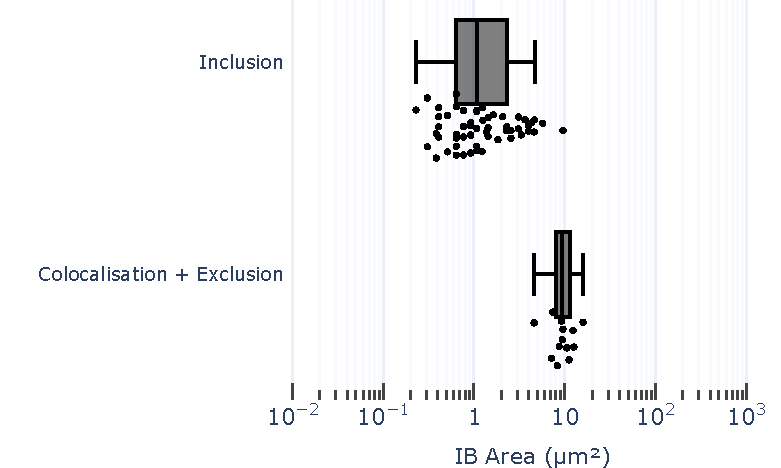
\includegraphics[width=1\linewidth]{08. Chapter 3/Figs/02. Infection/02. IFIT2/01. IFIT2A/08. box_i2a_a549-m21.pdf}
    \end{subfigure}
    \caption[Phenotypic Diversity of hIFIT2 Interactions with M2/1-Stained hRSV Inclusion Bodies, Detected by IFIT2A Antibody in A549 Cell Line.]{\textbf{Phenotypic Diversity of hIFIT2 Interactions with M2/1-Stained hRSV Inclusion Bodies, Detected by IFIT2A Antibody in A549 Cell Line.} A549 cells were infected with human RSV at MOI 1 and fixed 24 HPI. Cells were labeled with anti-RSV M2/1 and anti-IFIT2A antibodies and imaged on confocal microscope. Panel (a) shows percentual proportions of observed phenotypes between hRSV inclusion bodies and hIFIT2, detected by IFIT2A antibody (69 observations), with the red dotted line denoting the 5\% threshold, marking phenotypes considered relevant above this limit. Panel (b) shows the IB area in \(\mu m^2\) per observed relevant phenotype.}
    \label{fig:Phenotypic Diversity of hIFIT2 Interactions with M2/1-Stained hRSV Inclusion Bodies, Detected by IFIT2A Antibody in A549 Cell Line}
\end{figure}

\begin{figure}
    \centering
    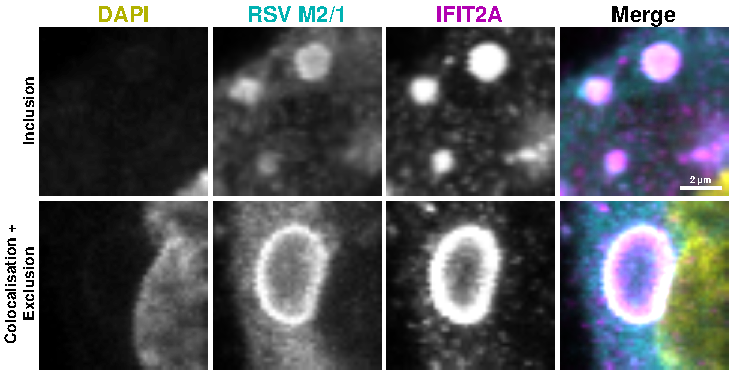
\includegraphics[width=1\linewidth]{08. Chapter 3/Figs/02. Infection/02. IFIT2/01. IFIT2A/09. i2a a549 hrsv m21.pdf} 
    \caption[Representative Images of Phenotypic Diversity of hIFIT2 Interactions with M2/1-Stained hRSV Inclusion Bodies, Detected by IFIT2A Antibody in A549 Cell Line.]{\textbf{Representative Images of Phenotypic Diversity of hIFIT2 Interactions with M2/1-Stained hRSV Inclusion Bodies, Detected by IFIT2A Antibody in A549 Cell Line.} A549 cells were infected with hRSV at MOI 1 and fixed at 24 HPI. Cellular nuclei were stained with DAPI (yellow), and cells were double-labeled with anti-RSV M2/1 (cyan) and anti-IFIT2A (magenta) antibodies. This figure showcases representative examples of relevant phenotypes in the interaction between hIFIT2, detected by IFIT2A antibody, and hRSV inclusion bodies. These phenotypes are presented in descending order based on their percentage proportions. The scale bar indicates 2 \(\mu m\).}
    \label{fig:Representative Images of Phenotypic Diversity of hIFIT2 Interactions with M2/1-Stained hRSV Inclusion Bodies, Detected by IFIT2A Antibody in A549 Cell Line}
\end{figure}

81 19

1 10

\begin{figure}
    \begin{subfigure}{0.495\textwidth}
        \caption{}
        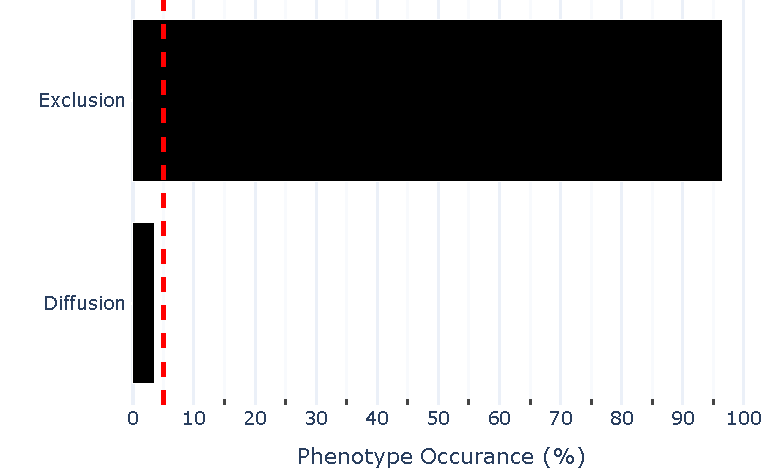
\includegraphics[width=1\linewidth]{08. Chapter 3/Figs/02. Infection/02. IFIT2/02. IFIT2B/01. bar_i2b_a549-n.pdf}
    \end{subfigure}
    \begin{subfigure}{0.495\textwidth}
        \caption{}
        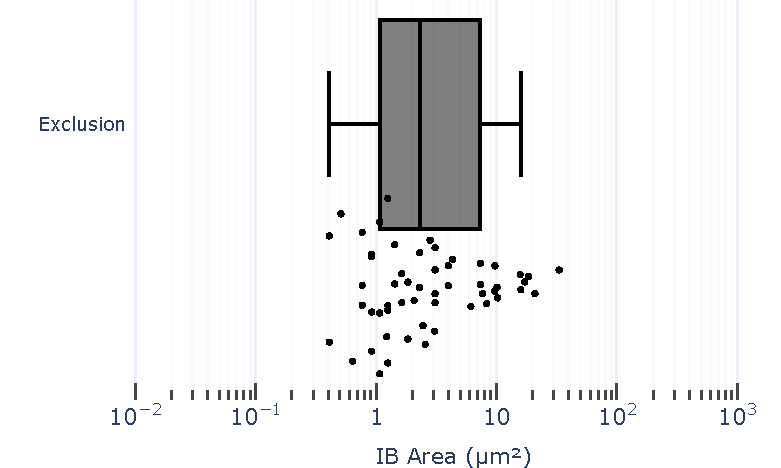
\includegraphics[width=1\linewidth]{08. Chapter 3/Figs/02. Infection/02. IFIT2/02. IFIT2B/02. box_i2b_a549-n.pdf}
    \end{subfigure}
    \caption[Phenotypic Diversity of hIFIT2 Interactions with Nucleoprotein-Stained hRSV Inclusion Bodies, Detected by IFIT2B Antibody in A549 Cell Line.]{\textbf{Phenotypic Diversity of hIFIT2 Interactions with Nucleoprotein-Stained hRSV Inclusion Bodies, Detected by IFIT2B Antibody in A549 Cell Line.} A549 cells were infected with human RSV at MOI 1 and fixed 24 HPI. Cells were labeled with anti-RSV N and anti-IFIT2B antibodies and imaged on confocal microscope. Panel (a) shows percentual proportions of observed phenotypes between hRSV inclusion bodies and hIFIT2, detected by IFIT2B antibody (56 observations), with the red dotted line denoting the 5\% threshold, marking phenotypes considered relevant above this limit. Panel (b) shows the IB area in \(\mu m^2\) per observed relevant phenotype.}
    \label{fig:Phenotypic Diversity of hIFIT2 Interactions with Nucleoprotein-Stained hRSV Inclusion Bodies, Detected by IFIT2B Antibody in A549 Cell Line}
\end{figure}

\begin{figure}
    \centering
    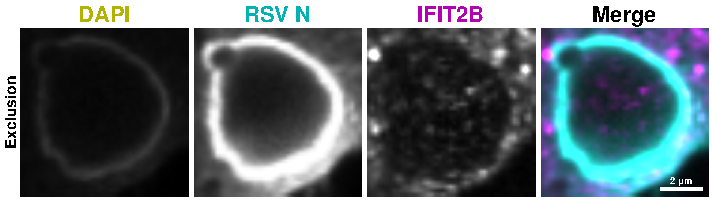
\includegraphics[width=1\linewidth]{08. Chapter 3/Figs/02. Infection/02. IFIT2/02. IFIT2B/03. i2b a549 hrsv n.pdf} 
    \caption[Representative Images of Phenotypic Diversity of hIFIT2 Interactions with Nucleoprotein-Stained hRSV Inclusion Bodies, Detected by IFIT2B Antibody in A549 Cell Line.]{\textbf{Representative Images of Phenotypic Diversity of hIFIT2 Interactions with Nucleoprotein-Stained hRSV Inclusion Bodies, Detected by IFIT2B Antibody in A549 Cell Line.} A549 cells were infected with hRSV at MOI 1 and fixed at 24 HPI. Cellular nuclei were stained with DAPI (yellow), and cells were double-labeled with anti-RSV N (cyan) and anti-IFIT2B (magenta) antibodies. This figure showcases representative examples of relevant phenotypes in the interaction between hIFIT2, detected by IFIT2B antibody, and hRSV inclusion bodies. These phenotypes are presented in descending order based on their percentage proportions. The scale bar indicates 2 \(\mu m\).}
    \label{fig:Representative Images of Phenotypic Diversity of hIFIT2 Interactions with Nucleoprotein-Stained hRSV Inclusion Bodies, Detected by IFIT2B Antibody in A549 Cell Line}
\end{figure}

96

2.1

Endogenous human IFIT2 is either partially excluded (top panel; decrease of intra IB signal compared to cytoplasmic signal) or completely excluded (bottom panel) from the human IB structure.

\begin{figure}
    \begin{subfigure}{0.495\textwidth}
        \caption{}
        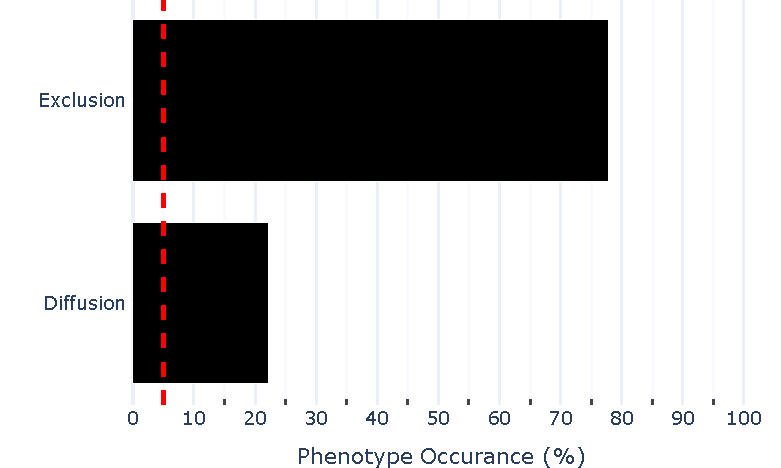
\includegraphics[width=1\linewidth]{08. Chapter 3/Figs/02. Infection/02. IFIT2/02. IFIT2B/04. bar_i2b_a549-p.pdf} 
    \end{subfigure}
    \begin{subfigure}{0.495\textwidth}
        \caption{}
        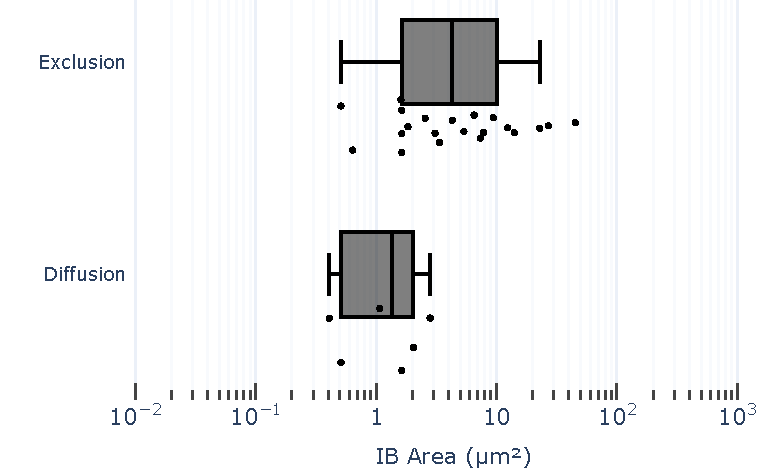
\includegraphics[width=1\linewidth]{08. Chapter 3/Figs/02. Infection/02. IFIT2/02. IFIT2B/05. box_i2b_a549-p.pdf}
    \end{subfigure}
    \caption[Phenotypic Diversity of hIFIT2 Interactions with Phosphoprotein-Stained hRSV Inclusion Bodies, Detected by IFIT2B Antibody in A549 Cell Line.]{\textbf{Phenotypic Diversity of hIFIT2 Interactions with Phosphoprotein-Stained hRSV Inclusion Bodies, Detected by IFIT2B Antibody in A549 Cell Line.} A549 cells were infected with human RSV at MOI 1 and fixed 24 HPI. Cells were labeled with anti-RSV P and anti-IFIT2B antibodies and imaged on confocal microscope. Panel (a) shows percentual proportions of observed phenotypes between hRSV inclusion bodies and hIFIT2, detected by IFIT2B antibody (27 observations), with the red dotted line denoting the 5\% threshold, marking phenotypes considered relevant above this limit. Panel (b) shows the IB area in \(\mu m^2\) per observed relevant phenotype.}
    \label{fig:Phenotypic Diversity of hIFIT2 Interactions with Phosphoprotein-Stained hRSV Inclusion Bodies, Detected by IFIT2B Antibody in A549 Cell Line}
\end{figure}

\begin{figure}
    \centering
    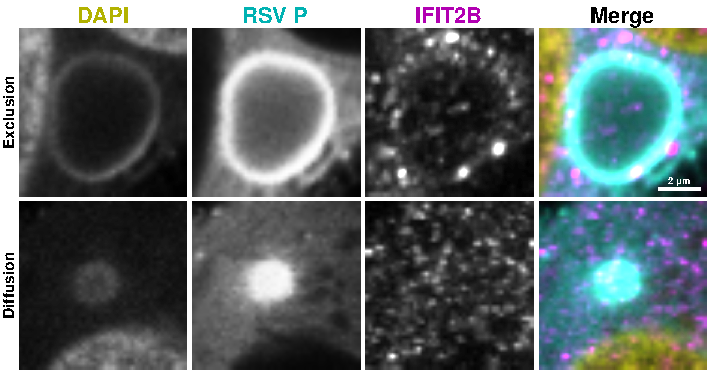
\includegraphics[width=1\linewidth]{08. Chapter 3/Figs/02. Infection/02. IFIT2/02. IFIT2B/06. i2b a549 hrsv p.pdf} 
    \caption[Representative Images of Phenotypic Diversity of hIFIT2 Interactions with Phosphoprotein-Stained hRSV Inclusion Bodies, Detected by IFIT2B Antibody in A549 Cell Line.]{\textbf{Representative Images of Phenotypic Diversity of hIFIT2 Interactions with Phosphoprotein-Stained hRSV Inclusion Bodies, Detected by IFIT2B Antibody in A549 Cell Line.} A549 cells were infected with hRSV at MOI 1 and fixed at 24 HPI. Cellular nuclei were stained with DAPI (yellow), and cells were double-labeled with anti-RSV P (cyan) and anti-IFIT2B (magenta) antibodies. This figure showcases representative examples of relevant phenotypes in the interaction between hIFIT2, detected by IFIT2B antibody, and hRSV inclusion bodies. These phenotypes are presented in descending order based on their percentage proportions. The scale bar indicates 2 \(\mu m\).}
    \label{fig:Representative Images of Phenotypic Diversity of hIFIT2 Interactions with Phosphoprotein-Stained hRSV Inclusion Bodies, Detected by IFIT2B Antibody in A549 Cell Line}
\end{figure}

78 22

4.3 1.3

We observe similar pattern of staining to what was observed with N stained human IBs. IFIT2 signal is either partially or totally excluded from the IB structure.

\begin{figure}
    \begin{subfigure}{0.495\textwidth}
        \caption{}
        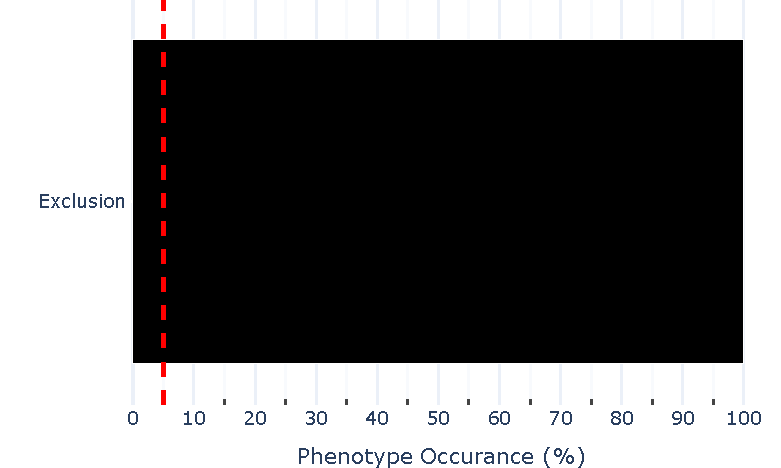
\includegraphics[width=1\linewidth]{08. Chapter 3/Figs/02. Infection/02. IFIT2/02. IFIT2B/07. bar_i2b_a549-m21.pdf} 
    \end{subfigure}
    \begin{subfigure}{0.495\textwidth}
        \caption{}
        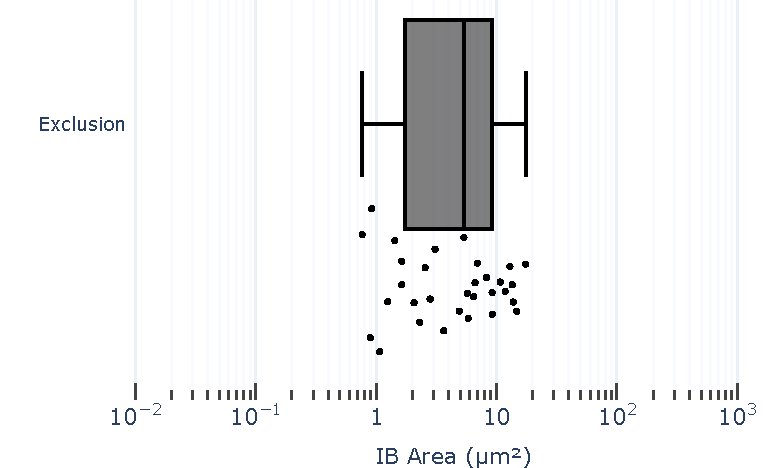
\includegraphics[width=1\linewidth]{08. Chapter 3/Figs/02. Infection/02. IFIT2/02. IFIT2B/08. box_i2b_a549-m21.pdf}
    \end{subfigure}
    \caption[Phenotypic Diversity of hIFIT2 Interactions with M2/1-Stained hRSV Inclusion Bodies, Detected by IFIT2B Antibody in A549 Cell Line.]{\textbf{Phenotypic Diversity of hIFIT2 Interactions with M2/1-Stained hRSV Inclusion Bodies, Detected by IFIT2B Antibody in A549 Cell Line.} A549 cells were infected with human RSV at MOI 1 and fixed 24 HPI. Cells were labeled with anti-RSV M2/1 and anti-IFIT2B antibodies and imaged on confocal microscope. Panel (a) shows percentual proportions of observed phenotypes between hRSV inclusion bodies and hIFIT2, detected by IFIT2B antibody (31 observations), with the red dotted line denoting the 5\% threshold, marking phenotypes considered relevant above this limit. Panel (b) shows the IB area in \(\mu m^2\) per observed relevant phenotype.}
    \label{fig:Phenotypic Diversity of hIFIT2 Interactions with M2/1-Stained hRSV Inclusion Bodies, Detected by IFIT2B Antibody in A549 Cell Line}
\end{figure}

\begin{figure}
    \centering
    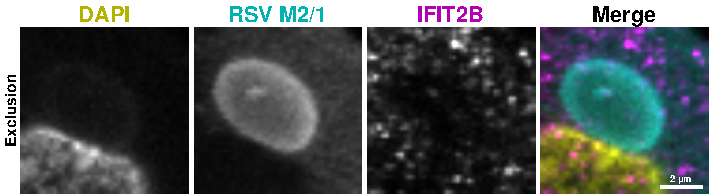
\includegraphics[width=1\linewidth]{08. Chapter 3/Figs/02. Infection/02. IFIT2/02. IFIT2B/09. i2b a549 hrsv m21.pdf} 
    \caption[Representative Images of Phenotypic Diversity of hIFIT2 Interactions with M2/1-Stained hRSV Inclusion Bodies, Detected by IFIT2B Antibody in A549 Cell Line.]{\textbf{Representative Images of Phenotypic Diversity of hIFIT2 Interactions with M2/1-Stained hRSV Inclusion Bodies, Detected by IFIT2B Antibody in A549 Cell Line.} A549 cells were infected with hRSV at MOI 1 and fixed at 24 HPI. Cellular nuclei were stained with DAPI (yellow), and cells were double-labeled with anti-RSV M2/1 (cyan) and anti-IFIT2B (magenta) antibodies. This figure showcases representative examples of relevant phenotypes in the interaction between hIFIT2, detected by IFIT2B antibody, and hRSV inclusion bodies. These phenotypes are presented in descending order based on their percentage proportions. The scale bar indicates 2 \(\mu m\).}
    \label{fig:Representative Images of Phenotypic Diversity of hIFIT2 Interactions with M2/1-Stained hRSV Inclusion Bodies, Detected by IFIT2B Antibody in A549 Cell Line}
\end{figure}

71 21 6

2.1 8 15

Endogenous human IFIT2 seems to be excluded from hRSV IBs.

\begin{figure}
    \begin{subfigure}{0.495\textwidth}
        \caption{}
        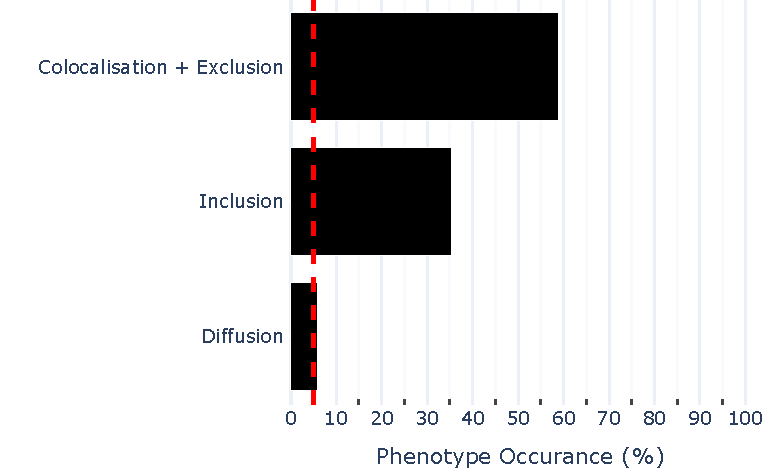
\includegraphics[width=1\linewidth]{08. Chapter 3/Figs/02. Infection/02. IFIT2/01. IFIT2A/10. bar_i2a_beas2b.pdf} 
    \end{subfigure}
    \begin{subfigure}{0.495\textwidth}
        \caption{}
        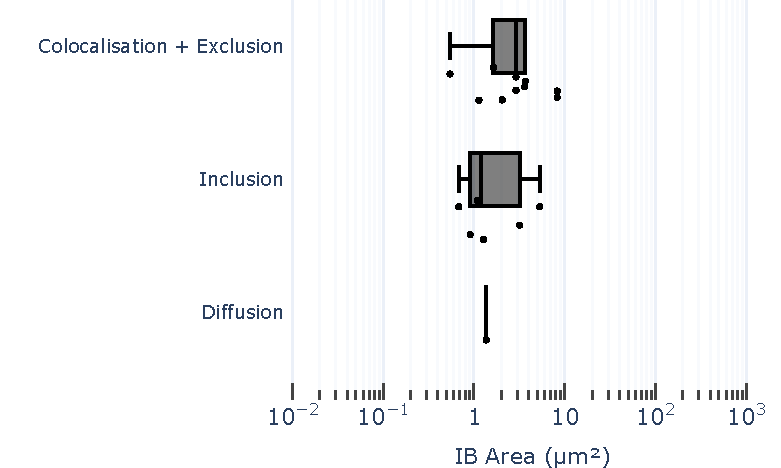
\includegraphics[width=1\linewidth]{08. Chapter 3/Figs/02. Infection/02. IFIT2/01. IFIT2A/11. box_i2a_beas2b.pdf}
    \end{subfigure}
    \caption[Phenotypic Diversity of hIFIT2 Interactions with hRSV Inclusion Bodies, Detected by IFIT2A Antibody in BEAS2B Cell Line.]{\textbf{Phenotypic Diversity of hIFIT2 Interactions with hRSV Inclusion Bodies, Detected by IFIT2A Antibody in BEAS2B Cell Line.} BEAS2B cells were infected with human RSV at MOI 1 and fixed 24 HPI. Cells were labeled with anti-RSV N and anti-IFIT2A antibodies and imaged on confocal microscope. Panel (a) shows percentual proportions of observed phenotypes between hRSV inclusion bodies and hIFIT2, detected by IFIT2A antibody (99 observations), with the red dotted line denoting the 5\% threshold, marking phenotypes considered relevant above this limit. Panel (b) shows the IB area in \(\mu m^2\) per observed relevant phenotype.}
    \label{fig:Phenotypic Diversity of hIFIT2 Interactions with hRSV Inclusion Bodies, Detected by IFIT2A Antibody in BEAS2B Cell Line}
\end{figure}

\begin{figure}
    \centering
    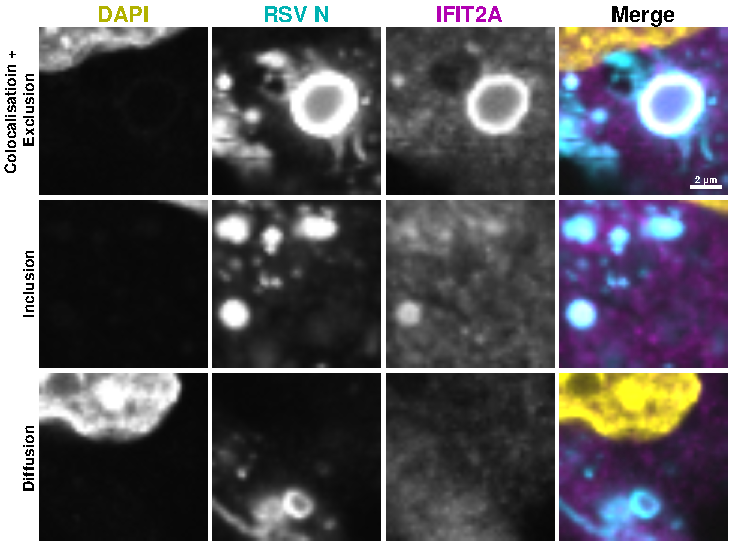
\includegraphics[width=1\linewidth]{08. Chapter 3/Figs/02. Infection/02. IFIT2/01. IFIT2A/12. i2a beas2b.pdf} 
    \caption[Representative Images of Phenotypic Diversity of hIFIT2 Interactions with hRSV Inclusion Bodies, Detected by IFIT2A Antibody in BEAS2B Cell Line.]{\textbf{Representative Images of Phenotypic Diversity of hIFIT2 Interactions with hRSV Inclusion Bodies, Detected by IFIT2A Antibody in BEAS2B Cell Line.} BEAS2B cells were infected with hRSV at MOI 1 and fixed at 24 HPI. Cellular nuclei were stained with DAPI (yellow), and cells were double-labeled with anti-RSV N (cyan) and anti-IFIT2A (magenta) antibodies. This figure showcases representative examples of relevant phenotypes in the interaction between hIFIT2, detected by IFIT2A antibody, and hRSV inclusion bodies. These phenotypes are presented in descending order based on their percentage proportions. The scale bar indicates 2 \(\mu m\).}
    \label{fig:Representative Images of Phenotypic Diversity of hIFIT2 Interactions with hRSV Inclusion Bodies, Detected by IFIT2A Antibody in BEAS2B Cell Line}
\end{figure}

58 35 5

3 1.2 1.2


Nascent bovine IFIT2 colocalization with regards of N stained bRSV IBs seems to strongly associate with the ring of the structure.

\begin{figure}
    \begin{subfigure}{0.495\textwidth}
        \caption{}
        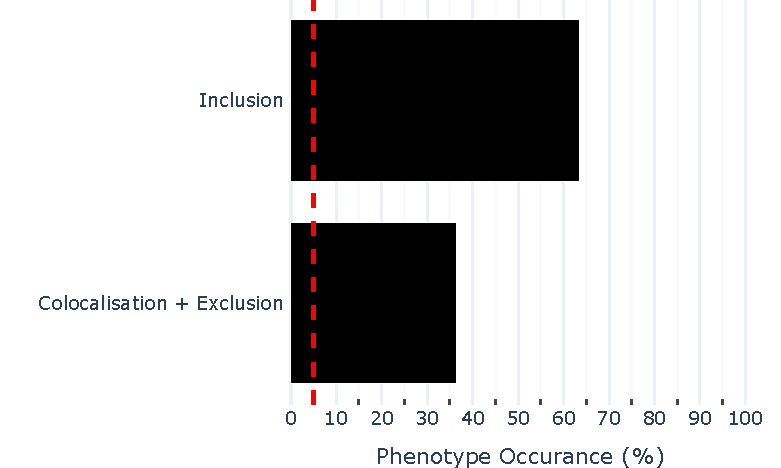
\includegraphics[width=1\linewidth]{08. Chapter 3/Figs/02. Infection/02. IFIT2/01. IFIT2A/13. bar_i2a_mdbk.pdf} 
    \end{subfigure}
    \begin{subfigure}{0.495\textwidth}
        \caption{}
        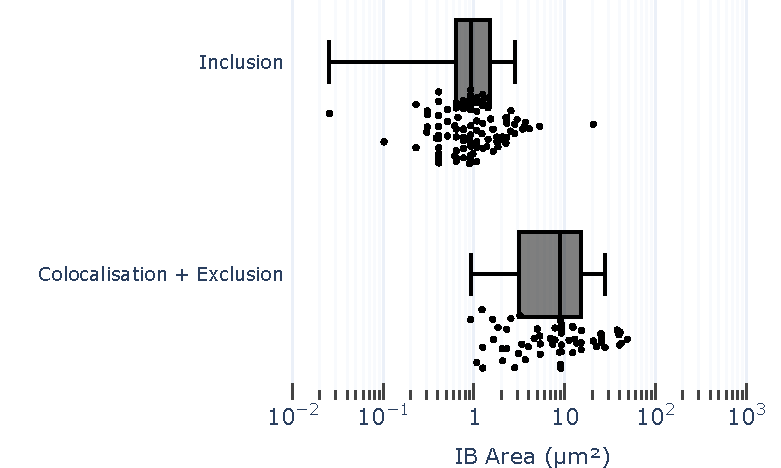
\includegraphics[width=1\linewidth]{08. Chapter 3/Figs/02. Infection/02. IFIT2/01. IFIT2A/14. box_i2a_mdbk.pdf}
    \end{subfigure}
    \caption[Phenotypic Diversity of hIFIT2 Interactions with bRSV Inclusion Bodies, Detected by IFIT2A Antibody in MDBK Cell Line.]{\textbf{Phenotypic Diversity of hIFIT2 Interactions with bRSV Inclusion Bodies, Detected by IFIT2A Antibody in MDBK Cell Line.} MDBK cells were infected with bovine RSV at MOI 1 and fixed 24 HPI. Cells were labeled with anti-RSV N and anti-IFIT2A antibodies and imaged on confocal microscope. Panel (a) shows percentual proportions of observed phenotypes between bRSV inclusion bodies and bIFIT2, detected by IFIT2A antibody (162 observations), with the red dotted line denoting the 5\% threshold, marking phenotypes considered relevant above this limit. Panel (b) shows the IB area in \(\mu m^2\) per observed relevant phenotype.}
    \label{fig:Phenotypic Diversity of hIFIT2 Interactions with bRSV Inclusion Bodies, Detected by IFIT2A Antibody in MDBK Cell Line}
\end{figure}

\begin{figure}
    \centering
    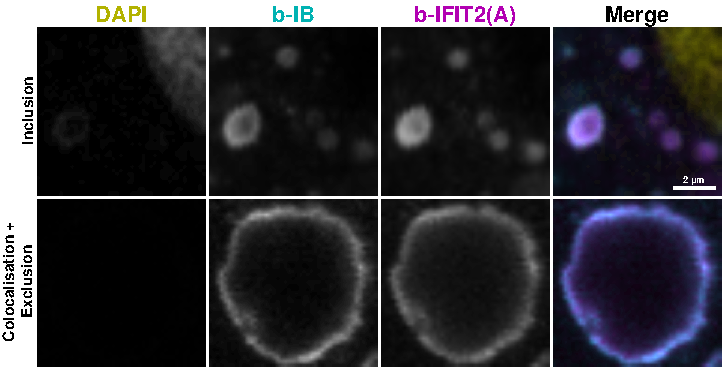
\includegraphics[width=1\linewidth]{08. Chapter 3/Figs/02. Infection/02. IFIT2/01. IFIT2A/15. i2a mdbk brsv.pdf} 
    \caption[Representative Images of Phenotypic Diversity of hIFIT2 Interactions with bRSV Inclusion Bodies, Detected by IFIT2A Antibody in MDBK Cell Line.]{\textbf{Representative Images of Phenotypic Diversity of hIFIT2 Interactions with bRSV Inclusion Bodies, Detected by IFIT2A Antibody in MDBK Cell Line.} MDBK cells were infected with bRSV at MOI 1 and fixed at 24 HPI. Cellular nuclei were stained with DAPI (yellow), and cells were double-labeled with anti-RSV N (cyan) and anti-IFIT2A (magenta) antibodies. This figure showcases representative examples of relevant phenotypes in the interaction between bIFIT2, detected by IFIT2A antibody, and bRSV inclusion bodies. These phenotypes are presented in descending order based on their percentage proportions. The scale bar indicates 2 \(\mu m\).}
    \label{fig:Representative Images of Phenotypic Diversity of hIFIT2 Interactions with bRSV Inclusion Bodies, Detected by IFIT2A Antibody in MDBK Cell Line}
\end{figure}

64 36

1 9

\begin{figure}
    \begin{subfigure}{0.495\textwidth}
        \caption{}
        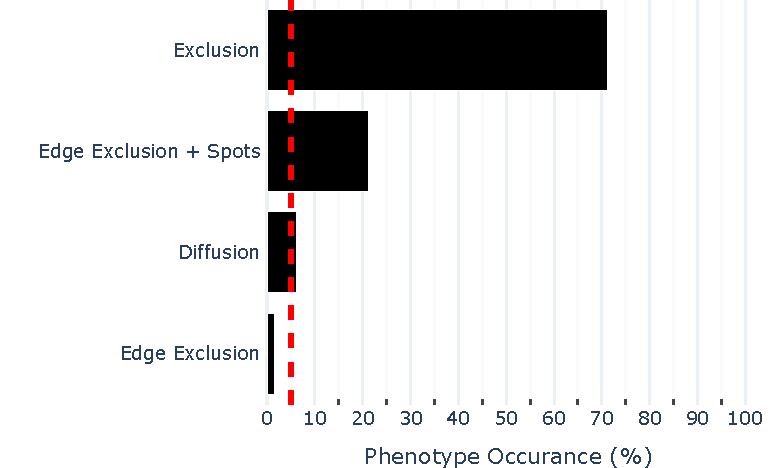
\includegraphics[width=1\linewidth]{08. Chapter 3/Figs/02. Infection/02. IFIT2/02. IFIT2B/10. bar_i2b_mdbk.pdf} 
    \end{subfigure}
    \begin{subfigure}{0.495\textwidth}
        \caption{}
        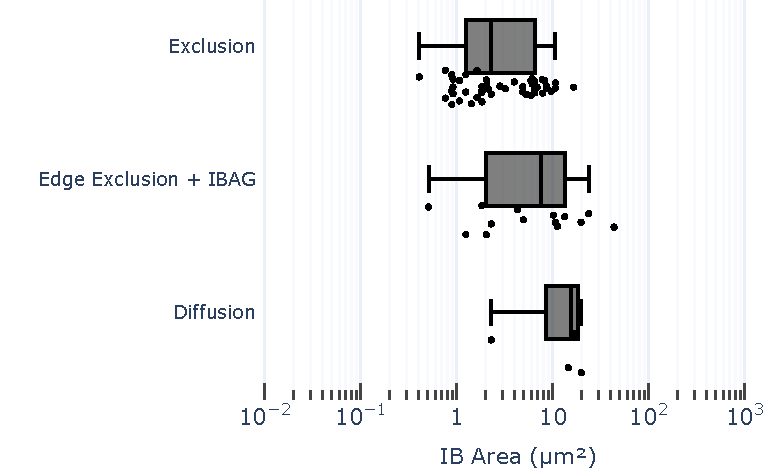
\includegraphics[width=1\linewidth]{08. Chapter 3/Figs/02. Infection/02. IFIT2/02. IFIT2B/11. box_i2b_mdbk.pdf}
    \end{subfigure}
    \caption[Phenotypic Diversity of hIFIT2 Interactions with bRSV Inclusion Bodies, Detected by IFIT2B Antibody in MDBK Cell Line.]{\textbf{Phenotypic Diversity of hIFIT2 Interactions with bRSV Inclusion Bodies, Detected by IFIT2B Antibody in MDBK Cell Line.} MDBK cells were infected with bovine RSV at MOI 1 and fixed 24 HPI. Cells were labeled with anti-RSV N and anti-IFIT2B antibodies and imaged on confocal microscope. Panel (a) shows percentual proportions of observed phenotypes between bRSV inclusion bodies and bIFIT2, detected by IFIT2B antibody (66 observations), with the red dotted line denoting the 5\% threshold, marking phenotypes considered relevant above this limit. Panel (b) shows the IB area in \(\mu m^2\) per observed relevant phenotype.}
    \label{fig:Phenotypic Diversity of hIFIT2 Interactions with bRSV Inclusion Bodies, Detected by IFIT2B Antibody in MDBK Cell Line}
\end{figure}

\begin{figure}
    \centering
    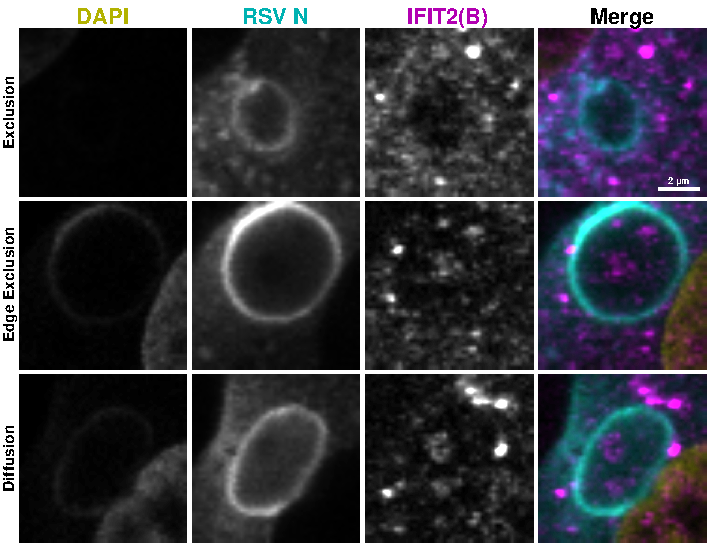
\includegraphics[width=1\linewidth]{08. Chapter 3/Figs/02. Infection/02. IFIT2/02. IFIT2B/12. i2b mdbk brsv.pdf} 
    \caption[Representative Images of Phenotypic Diversity of hIFIT2 Interactions with bRSV Inclusion Bodies, Detected by IFIT2B Antibody in MDBK Cell Line.]{\textbf{Representative Images of Phenotypic Diversity of hIFIT2 Interactions with bRSV Inclusion Bodies, Detected by IFIT2B Antibody in MDBK Cell Line.} MDBK cells were infected with bRSV at MOI 1 and fixed at 24 HPI. Cellular nuclei were stained with DAPI (yellow), and cells were double-labeled with anti-RSV N (cyan) and anti-IFIT2B (magenta) antibodies. This figure showcases representative examples of relevant phenotypes in the interaction between bIFIT2, detected by IFIT2B antibody, and bRSV inclusion bodies. These phenotypes are presented in descending order based on their percentage proportions. The scale bar indicates 2 \(\mu m\).}
    \label{fig:Representative Images of Phenotypic Diversity of hIFIT2 Interactions with bRSV Inclusion Bodies, Detected by IFIT2B Antibody in MDBK Cell Line}
\end{figure}

71 21 6

2 8 17

\subsubsection{Phenotypic Diversity of Nascent IFIT3 Interaction with RSV Inclusion Bodies}
Nascent human IFIT3 seems to have mainly diffused phenotype (top and bottom panel) with occasional exclusion without any marked IFIT3 concentration adjacent to the IB structure (middle panel).

53, 17, 16, 10

4.5, 12, 5, 1.9

\begin{figure}
    \begin{subfigure}{0.495\textwidth}
        \caption{}
        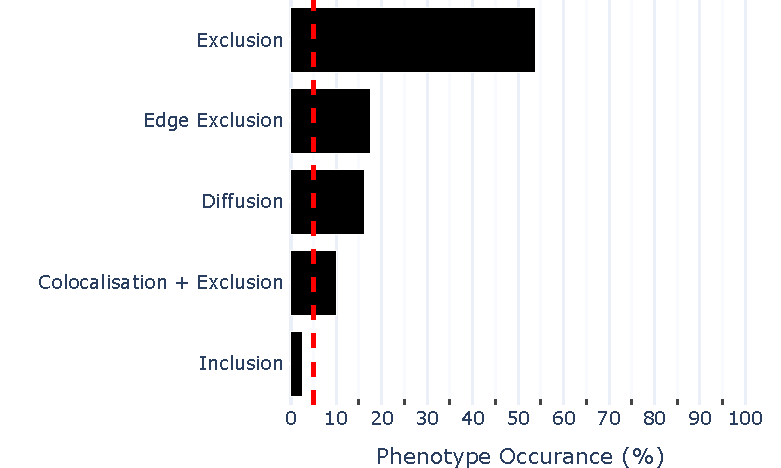
\includegraphics[width=1\linewidth]{08. Chapter 3/Figs/02. Infection/03. IFIT3/01. bar_i3_a549.pdf} 
    \end{subfigure}
    \begin{subfigure}{0.495\textwidth}
        \caption{}
        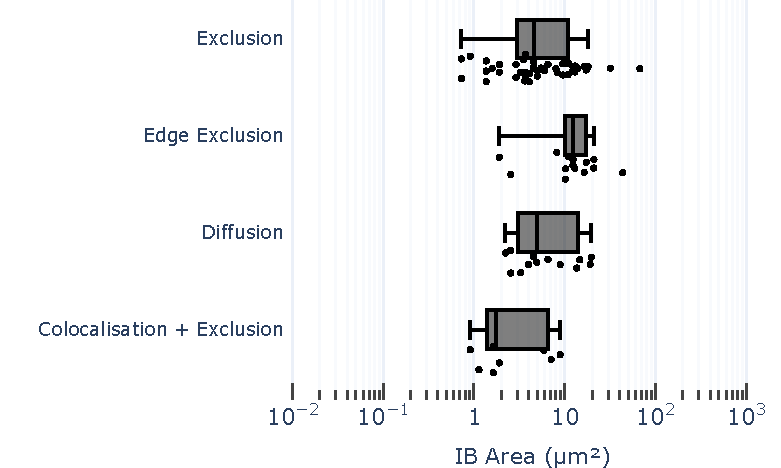
\includegraphics[width=1\linewidth]{08. Chapter 3/Figs/02. Infection/03. IFIT3/02. box_i3_a549.pdf}
    \end{subfigure}
    \caption[Phenotypic Diversity of hIFIT3 Interactions with hRSV Inclusion Bodies in A549 Cell Line.]{\textbf{Phenotypic Diversity of hIFIT3 Interactions with hRSV Inclusion Bodies in A549 Cell Line.} A549 cells were infected with human RSV at MOI 1 and fixed 24 HPI. Cells were double-labeled with with anti-RSV N and anti-IFIT3 antibodies and imaged on confocal microscope. Panel (a) shows percentual proportions of observed phenotypes between hRSV inclusion bodies and hIFIT3 (80 observations), with the red dotted line denoting the 5\% threshold, marking phenotypes considered relevant above this limit. Panel (b) shows the IB area in \(\mu m^2\) per observed relevant phenotype.}
    \label{fig:Phenotypic Diversity of hIFIT3 Interactions with hRSV Inclusion Bodies in A549 Cell Line}
\end{figure}

\begin{figure}
    \centering
    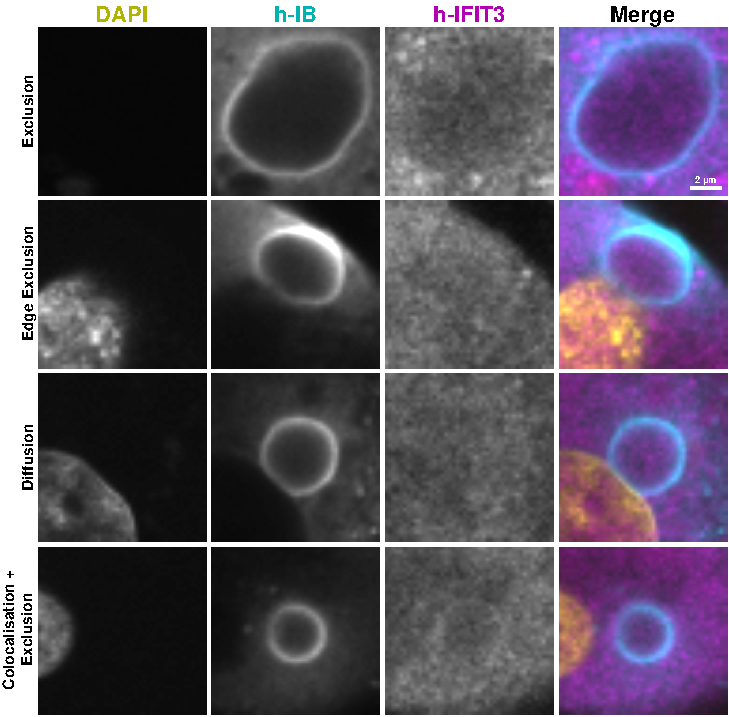
\includegraphics[width=1\linewidth]{08. Chapter 3/Figs/02. Infection/03. IFIT3/03. a549 i3.pdf}
    \caption[Representative Images of Phenotypic Diversity of hIFIT3 Interactions with hRSV Inclusion Bodies in A549 Cell Line.]{\textbf{Representative Images of Phenotypic Diversity of hIFIT3 Interactions with hRSV Inclusion Bodies in A549 Cell Line.} A549 cells were infected with hRSV at MOI 1 and fixed at 24 HPI. Cellular nuclei were stained with DAPI (yellow), and cells were double-labeled with anti-RSV N (cyan) and anti-IFIT3 (magenta) antibodies. This figure showcases representative examples of relevant phenotypes in the interaction between hIFIT3 and hRSV inclusion bodies. These phenotypes are presented in descending order based on their percentage proportions. The scale bar indicates 2 \(\mu m\).}
    \label{fig:Representative Images of Phenotypic Diversity of hIFIT3 Interactions with hRSV Inclusion Bodies in A549 Cell Line}
\end{figure}

62, 19, 12

5.5, 3, 10, 2.3

\begin{figure}
    \begin{subfigure}{0.495\textwidth}
        \caption{}
        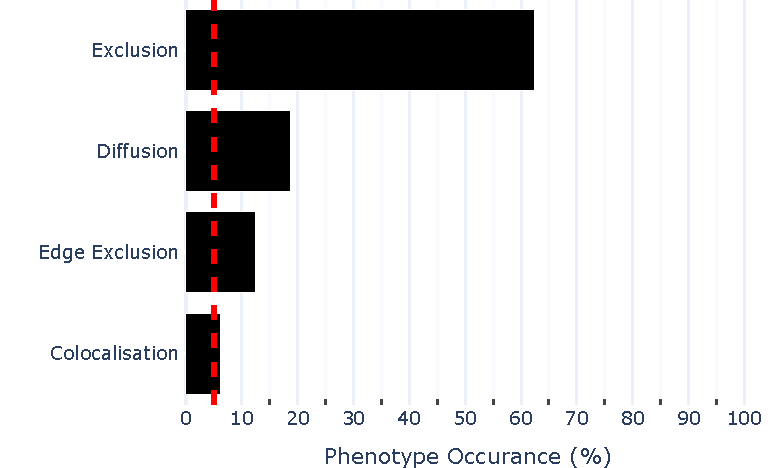
\includegraphics[width=1\linewidth]{08. Chapter 3/Figs/02. Infection/03. IFIT3/04. bar_i3_beas2b.pdf} 
    \end{subfigure}
    \begin{subfigure}{0.495\textwidth}
        \caption{}        
        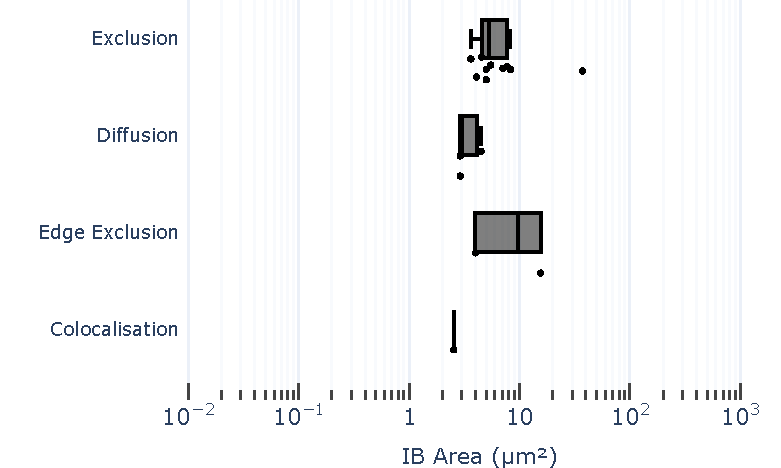
\includegraphics[width=1\linewidth]{08. Chapter 3/Figs/02. Infection/03. IFIT3/05. box_i3_beas2b.pdf}
    \end{subfigure}
    \caption[Phenotypic Diversity of hIFIT3 Interactions with hRSV Inclusion Bodies in BEAS2B Cell Line.]{\textbf{Phenotypic Diversity of hIFIT3 Interactions with hRSV Inclusion Bodies in BEAS2B Cell Line.} BEAS2B cells were infected with human RSV at MOI 1 and fixed 24 HPI. Cells were labeled with anti-RSV N and anti-IFIT3 antibodies and imaged on confocal microscope. Panel (a) shows percentual proportions of observed phenotypes between hRSV inclusion bodies and hIFIT3 (16 observations), with the red dotted line denoting the 5\% threshold, marking phenotypes considered relevant above this limit. Panel (b) shows the IB area in \(\mu m^2\) per observed relevant phenotype.}
    \label{fig:Phenotypic Diversity of hIFIT3 Interactions with hRSV Inclusion Bodies in BEAS2B Cell Line}
\end{figure}

\begin{figure}
    \centering
    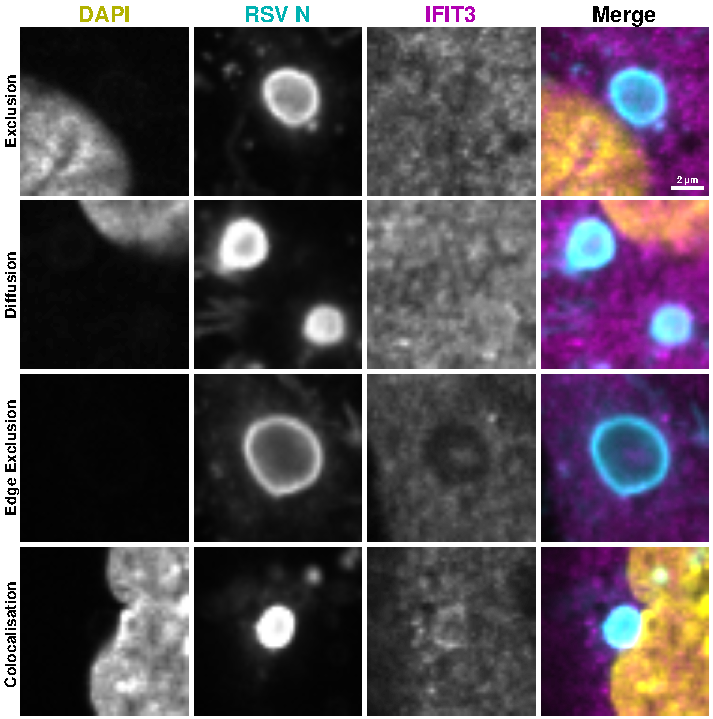
\includegraphics[width=1\linewidth]{08. Chapter 3/Figs/02. Infection/03. IFIT3/06. beas2b i3.pdf}
    \caption[Representative Images of Phenotypic Diversity of hIFIT3 Interactions with hRSV Inclusion Bodies in BEAS2B Cell Line]{\textbf{Representative Images of Phenotypic Diversity of hIFIT3 Interactions with hRSV Inclusion Bodies in BEAS2B Cell Line.} BEAS2B cells were infected with hRSV at MOI 1 and fixed at 24 HPI. Cellular nuclei were stained with DAPI (yellow), and cells were double-labeled with anti-RSV N (cyan) and anti-IFIT3 (magenta) antibodies. This figure showcases representative examples of relevant phenotypes in the interaction between hIFIT3 and hRSV inclusion bodies. These phenotypes are presented in descending order based on their percentage proportions. The scale bar indicates 2 \(\mu m\).}
    \label{fig:Representative Images of Phenotypic Diversity of hIFIT3 Interactions with hRSV Inclusion Bodies in BEAS2B Cell Line}
\end{figure}

43, 34, 11, 8

1.1, 3.3, 1, 11

\begin{figure}
    \begin{subfigure}{0.495\textwidth}
        \caption{}
        \includegraphics[width=1\linewidth]{08. Chapter 3/Figs/02. Infection/03. IFIT3/07. bar_i3_mdbk.pdf} 
    \end{subfigure}
    \begin{subfigure}{0.495\textwidth}
        \caption{}
        \includegraphics[width=1\linewidth]{08. Chapter 3/Figs/02. Infection/03. IFIT3/08. box_i3_mdbk.pdf}
    \end{subfigure}
    \caption[Phenotypic Diversity of bIFIT3 Interactions with bRSV Inclusion Bodies in MDBK Cell Line.]{\textbf{Phenotypic Diversity of bIFIT3 Interactions with bRSV Inclusion Bodies in MDBK Cell Line.} MDBK cells were infected with bovine RSV at MOI 1 and fixed 24 HPI. Cells were labeled with anti-RSV N and anti-IFIT3 antibodies and imaged on confocal microscope. Panel (a) shows percentual proportions of observed phenotypes between bRSV inclusion bodies and bIFIT3 (214 observations), with the red dotted line denoting the 5\% threshold, marking phenotypes considered relevant above this limit. Panel (b) shows the IB area in \(\mu m^2\) per observed relevant phenotype.}
    \label{fig:Phenotypic Diversity of bIFIT3 Interactions with bRSV Inclusion Bodies in MDBK Cell Line}
\end{figure}

\begin{figure}
    \centering
    \includegraphics[width=1\linewidth]{08. Chapter 3/Figs/02. Infection/03. IFIT3/09. mdbk i3.pdf}
    \caption[Representative Images of Phenotypic Diversity of bIFIT3 Interactions with bRSV Inclusion Bodies in MDBK Cell Line.]{\textbf{Representative Images of Phenotypic Diversity of bIFIT3 Interactions with bRSV Inclusion Bodies in MDBK Cell Line.} MDBK cells were infected with bRSV at MOI 1 and fixed at 24 HPI. Cellular nuclei were stained with DAPI (yellow), and cells were double-labeled with anti-RSV N (cyan) and anti-IFIT3 (magenta) antibodies. This figure showcases representative examples of relevant phenotypes in the interaction between bIFIT3 and bRSV inclusion bodies. These phenotypes are presented in descending order based on their percentage proportions. The scale bar indicates 2 \(\mu m\).}
    \label{fig:Representative Images of Phenotypic Diversity of bIFIT3 Interactions with bRSV Inclusion Bodies in MDBK Cell Line}
\end{figure}

\subsubsection{Phenotypic Diversity of Nascent IFIT5 Interaction with RSV Inclusion Bodies}
hIFIT5 seems to be excluded from hRSV IBs. There is a hint of accumulation of IFIT5 on the outside of IB (bottom panel; no z stacks to confirm this). 

58, 17, 16, 5

6.3, 4, 8, 13

\begin{figure}
    \begin{subfigure}{0.495\textwidth}
        \caption{}
        \includegraphics[width=1\linewidth]{08. Chapter 3/Figs/02. Infection/04. IFIT5/01. bar_i5_a549.pdf} 
    \end{subfigure}
    \begin{subfigure}{0.495\textwidth}
        \caption{}
        \includegraphics[width=1\linewidth]{08. Chapter 3/Figs/02. Infection/04. IFIT5/02. box_i5_a549.pdf}
    \end{subfigure}
    \caption[Phenotypic Diversity of hIFIT5 Interactions with hRSV Inclusion Bodies in A549 Cell Line.]{\textbf{Phenotypic Diversity of hIFIT5 Interactions with hRSV Inclusion Bodies in A549 Cell Line.} A549 cells were infected with human RSV at MOI 1 and fixed 24 HPI. Cells were labeled with anti-RSV N and anti-IFIT5 antibodies and imaged on confocal microscope. Panel (a) shows percentual proportions of observed phenotypes between hRSV inclusion bodies and hIFIT5 (77 observations), with the red dotted line denoting the 5\% threshold, marking phenotypes considered relevant above this limit. Panel (b) shows the IB area in \(\mu m^2\) per observed relevant phenotype.}
    \label{fig:Phenotypic Diversity of hIFIT5 Interactions with hRSV Inclusion Bodies in A549 Cell Line}
\end{figure}

\begin{figure}
    \centering
    \includegraphics[width=1\linewidth]{08. Chapter 3/Figs/02. Infection/04. IFIT5/03. a549 i5.pdf}
    \caption[Representative Images of Phenotypic Diversity of hIFIT5 Interactions with hRSV Inclusion Bodies in A549 Cell Line.]{\textbf{Representative Images of Phenotypic Diversity of hIFIT5 Interactions with hRSV Inclusion Bodies in A549 Cell Line.} A549 cells were infected with hRSV at MOI 1 and fixed at 24 HPI. Cellular nuclei were stained with DAPI (yellow), and cells were double-labeled with anti-RSV N (cyan) and anti-IFIT5 (magenta) antibodies. This figure showcases representative examples of relevant phenotypes in the interaction between hIFIT5 and hRSV inclusion bodies. These phenotypes are presented in descending order based on their percentage proportions. The scale bar indicates 2 \(\mu m\).}
    \label{fig:Representative Images of Phenotypic Diversity of hIFIT5 Interactions with hRSV Inclusion Bodies in A549 Cell Line}
\end{figure}

62, 18, 18

2, 2.3, 3

\begin{figure}
    \begin{subfigure}{0.495\textwidth}
        \caption{}
        \includegraphics[width=1\linewidth]{08. Chapter 3/Figs/02. Infection/04. IFIT5/04. bar_i5_beas2b.pdf}
    \end{subfigure}
    \begin{subfigure}{0.495\textwidth}
        \caption{}
        \includegraphics[width=1\linewidth]{08. Chapter 3/Figs/02. Infection/04. IFIT5/05. box_i5_beas2b.pdf}
    \end{subfigure}
    \caption[Phenotypic Diversity of hIFIT5 Interactions with hRSV Inclusion Bodies in BEAS2B Cell Line.]{\textbf{Phenotypic Diversity of hIFIT5 Interactions with hRSV Inclusion Bodies in BEAS2B Cell Line.} BEAS2B cells were infected with human RSV at MOI 1 and fixed 24 HPI. Cells were labeled with anti-RSV N and anti-IFIT5 antibodies and imaged on confocal microscope. Panel (a) shows percentual proportions of observed phenotypes between hRSV inclusion bodies and hIFIT5 (21 observations), with the red dotted line denoting the 5\% threshold, marking phenotypes considered relevant above this limit. Panel (b) shows the IB area in \(\mu m^2\) per observed relevant phenotype.}
    \label{fig:Phenotypic Diversity of hIFIT5 Interactions with hRSV Inclusion Bodies in BEAS2B Cell Line}
\end{figure}

\begin{figure}
    \centering
    \includegraphics[width=1\linewidth]{08. Chapter 3/Figs/02. Infection/04. IFIT5/06. beas2b i5.pdf}
    \caption[Representative Images of Phenotypic Diversity of hIFIT5 Interactions with hRSV Inclusion Bodies in BEAS2B Cell Line.]{\textbf{Representative Images of Phenotypic Diversity of hIFIT5 Interactions with hRSV Inclusion Bodies in BEAS2B Cell Line.} BEAS2B cells were infected with hRSV at MOI 1 and fixed at 24 HPI. Cellular nuclei were stained with DAPI (yellow), and cells were double-labeled with anti-RSV N (cyan) and anti-IFIT5 (magenta) antibodies. This figure showcases representative examples of relevant phenotypes in the interaction between hIFIT5 and hRSV inclusion bodies. These phenotypes are presented in descending order based on their percentage proportions. The scale bar indicates 2 \(\mu m\).}
    \label{fig:Representative Images of Phenotypic Diversity of hIFIT5 Interactions with hRSV Inclusion Bodies in BEAS2B Cell Line}
\end{figure}

51, 29, 10, 7

1, 10, 3, 0.9

\begin{figure}
    \begin{subfigure}{0.495\textwidth}
        \caption{}
        \includegraphics[width=1\linewidth]{08. Chapter 3/Figs/02. Infection/04. IFIT5/07. bar_i5_mdbk.pdf} 
    \end{subfigure}
    \begin{subfigure}{0.495\textwidth}
        \caption{}
        \includegraphics[width=1\linewidth]{08. Chapter 3/Figs/02. Infection/04. IFIT5/08. box_i5_mdbk.pdf}
    \end{subfigure}
    \caption[Phenotypic Diversity of bIFIT5 Interactions with bRSV Inclusion Bodies in MDBK Cell Line.]{\textbf{Phenotypic Diversity of bIFIT5 Interactions with bRSV Inclusion Bodies in MDBK Cell Line.} MDBK cells were infected with bovine RSV at MOI 1 and fixed 24 HPI. Cells were labeled with anti-RSV N and anti-IFIT5 antibodies and imaged on confocal microscope. Panel (a) shows percentual proportions of observed phenotypes between bRSV inclusion bodies and bIFIT5 (61 observations), with the red dotted line denoting the 5\% threshold, marking phenotypes considered relevant above this limit. Panel (b) shows the IB area in \(\mu m^2\) per observed relevant phenotype.}
    \label{fig:Phenotypic Diversity of bIFIT5 Interactions with bRSV Inclusion Bodies in MDBK Cell Line}
\end{figure}

\begin{figure}
    \centering
    \includegraphics[width=1\linewidth]{08. Chapter 3/Figs/02. Infection/04. IFIT5/09. mdbk i5.pdf}
    \caption[Representative Images of Phenotypic Diversity of bIFIT5 Interactions with bRSV Inclusion Bodies in MDBK Cell Line.]{\textbf{Representative Images of Phenotypic Diversity of bIFIT5 Interactions with bRSV Inclusion Bodies in MDBK Cell Line.} MDBK cells were infected with bRSV at MOI 1 and fixed at 24 HPI. Cellular nuclei were stained with DAPI (yellow), and cells were double-labeled with anti-RSV N (cyan) and anti-IFIT5 (magenta) antibodies. This figure showcases representative examples of relevant phenotypes in the interaction between bIFIT5 and bRSV inclusion bodies. These phenotypes are presented in descending order based on their percentage proportions. The scale bar indicates 2 \(\mu m\).}
    \label{fig:Representative Images of Phenotypic Diversity of bIFIT5 Interactions with bRSV Inclusion Bodies in MDBK Cell Line}
\end{figure}

% summary
In the context of infection, endogenous human IFIT1 concentrates within the human RSV IB structure; colocalises to the edge of the IB; is diffused through the structure and cytoplasm equally; or is excluded from the structure. This suggests that the interaction between human IFIT1 and hRSV IB is dynamic and depends on factors that we do not understand yet. In the case of endogenous bovine IFIT1 in the context of bRSV IBs, IFIT1 is either excluded from the structure; excluded from the IB inner edge but concentrated inside; or excluded from the centre of IB structure but concentrated on the inner edge of the structure. 

Nascent human IFIT3 during hRSV infection is either excluded from IB structure or is diffused through the structure. Occasionally it colocalises to the IB ring. Nascent bIFIT3 during bRSV infection either siphons inside IBs and shows sub-IB granules or is excluded from the IB boundary with slightly decreased signal inside of the IB.

In human cells during hRSV infection IFIT5 is mainly excluded from the IBs but seems to concentrate on their edge. Once we saw colocalization with the IB ring and a concentration of IFIT5 inside it. In bovine cells IFIT5 is always excluded from the IB boundary and the signal inside is either slightly decreased or equal compared to cytoplasmic IFIT5. 

\subsection{Nascent IFIT1, IFIT3, and IFIT5 Localisation in a Simplified System of pseudo-IBs} \label{subsec:Nascent IFIT1, IFIT3, and IFIT5 Localisation in a Simplified System of pseudo-IBs}

how we did pIBs and what they are
characterisation of pibs observed from our study

\begin{figure}
    \begin{subfigure}{0.495\textwidth}
        \caption{}
        \includegraphics[width=\textwidth]{08. Chapter 3/Figs/03. pIB/01. pIB characterisation/01. heatmap_pib-293t.pdf} 
    \end{subfigure}
    \hfill
    \begin{subfigure}{0.495\textwidth}
        \caption{}
        \includegraphics[width=\textwidth]{08. Chapter 3/Figs/03. pIB/01. pIB characterisation/02. heatmap_pib-vero.pdf}
    \end{subfigure}
    \caption[Size Characterization of Pseudo Inclusion Bodies Across Different Cell Lines.]{\textbf{Size Characterization of Pseudo Inclusion Bodies Across Different Cell Lines.} This figure presents the relationship between the measured area (\(\mu m^2\)) and diameter (\(\mu m\)) of individual pseudo inclusion bodies (pIBs) as observed within the scope of this study. Additionally, the figure includes distinct population distributions depicted alongside the plots, representing (a) 103
     o observations from the 293T cell line and (b) 1321 observations from the Vero cell line. Contour plots are incorporated to elucidate the underlying density of individual IBs within the plots.}
    \label{fig:Size Characterization of Pseudo Inclusion Bodies Across Different Cell Lines}
\end{figure}


\begin{figure}
    \centering
    \includegraphics[width=0.75\linewidth]{08. Chapter 3/Figs/03. pIB/01. pIB characterisation/03. box-pib.pdf}
    \caption[boxplot of pib sizes per cell line.]{\textbf{boxplot of pib sizes per cell line.} this is the data from above but only area, to be able to compare it later}
    \label{fig:boxplot of pib sizes per cell line}
\end{figure}

2.2, 1 


\subsubsection{pIB IFIT1}

\begin{figure}
    \begin{subfigure}{0.495\textwidth}
        \caption{}
        \includegraphics[width=1\linewidth]{08. Chapter 3/Figs/03. pIB/02. IFIT1/01. bar_i1_293t.pdf} 
    \end{subfigure}
    \begin{subfigure}{0.495\textwidth}
        \caption{}
        \includegraphics[width=1\linewidth]{08. Chapter 3/Figs/03. pIB/02. IFIT1/02. box_i1_293t.pdf}
    \end{subfigure}
    \caption[Diverse Phenotypic Interactions of Human IFIT1 with Human Pseudo Inclusion Bodies (pIBs) in the 293T Cell Line.]{\textbf{Diverse Phenotypic Interactions of Human IFIT1 with Human Pseudo Inclusion Bodies (pIBs) in the 293T Cell Line.} 293T cells were transfected with hRSV N and P containing plasmids using TransIT-X2 and were fixed after 24 hours. Cells were labeled with anti-RSV N and anti-IFIT1 antibodies and imaged on confocal microscope. Panel (a) shows percentual proportions of observed phenotypes between hRSV pseudo inclusion bodies and human IFIT1 (16 observations), with the red dotted line denoting the 5\% threshold, marking phenotypes considered relevant above this limit. Panel (b) shows the IB area in \(\mu m^2\) per observed relevant phenotype.}
    \label{fig:Diverse Phenotypic Interactions of Human IFIT1 with Human Pseudo Inclusion Bodies (pIBs) in the 293T Cell Line}
\end{figure}

\begin{figure}
    \centering
    \includegraphics[width=1\linewidth]{08. Chapter 3/Figs/03. pIB/02. IFIT1/03. i1-293t-hnhp.pdf}
    \caption[Representative Images of Diverse Phenotypic Interactions of Human IFIT1 with Human Pseudo Inclusion Bodies (pIBs) in the 293T Cell Line.]{\textbf{Representative Images of Diverse Phenotypic Interactions of Human IFIT1 with Human Pseudo Inclusion Bodies (pIBs) in the 293T Cell Line.} 293T cells were transfected with hRSV N and P containing plasmids using TransIT-X2 and were fixed after 24 hours. Cellular nuclei were stained with DAPI (yellow), and cells were double-labeled with anti-RSV N (cyan) and anti-IFIT1 (magenta) antibodies. This figure showcases representative examples of relevant phenotypes in the interaction between human IFIT1 and hRSV pseudo inclusion bodies. These phenotypes are presented in descending order based on their percentage proportions. The scale bar indicates 2 \(\mu m\).}
    \label{fig:Representative Images of Diverse Phenotypic Interactions of Human IFIT1 with Human Pseudo Inclusion Bodies (pIBs) in the 293T Cell Line}
\end{figure}

50 44 6

1, 2.5, 3.3


Nascent human IFIT1 seems to be diffused through the pIB structure i.e., the signal intensity and distribution between cytoplasmic and pIB staining is identical.  

Endogenous monkey IFIT1 displays colocalization with human pIB structures (top panel), or inclusion within the structures (bottom panel). Monkey IFIT1 signal is also excluded from the pIB filamentous network (top panel; shown by arrows). This suggests that the colocalization is not caused by mere interaction with N or P but its dependant on the integrity of pIBs. These data are supported by z stack measurements.  

\begin{figure}
    \begin{subfigure}{0.495\textwidth}
        \caption{}
        \includegraphics[width=1\linewidth]{08. Chapter 3/Figs/03. pIB/02. IFIT1/04. bar_i1_vero_hnhp.pdf} 
    \end{subfigure}
    \begin{subfigure}{0.495\textwidth}
        \caption{}
        \includegraphics[width=1\linewidth]{08. Chapter 3/Figs/03. pIB/02. IFIT1/05. box_i1_vero_hnhp.pdf}
    \end{subfigure}
    \caption[Diverse Phenotypic Interactions of Monkey IFIT1 with Human Pseudo Inclusion Bodies (pIBs) in the VERO Cell Line.]{\textbf{Diverse Phenotypic Interactions of Monkey IFIT1 with Human Pseudo Inclusion Bodies (pIBs) in the VERO Cell Line.} Vero cells were transfected with hRSV N and P containing plasmids using TransIT-X2 and were fixed after 24 hours. Cells were labeled with anti-RSV N and anti-IFIT1 antibodies and imaged on confocal microscope. Panel (a) shows percentual proportions of observed phenotypes between hRSV pseudo inclusion bodies and monkey IFIT1 (76 observations), with the red dotted line denoting the 5\% threshold, marking phenotypes considered relevant above this limit. Panel (b) shows the IB area in \(\mu m^2\) per observed relevant phenotype.}
    \label{fig:Diverse Phenotypic Interactions of Monkey IFIT1 with Human Pseudo Inclusion Bodies (pIBs) in the VERO Cell Line}
\end{figure}

\begin{figure}
    \centering
    \includegraphics[width=1\linewidth]{08. Chapter 3/Figs/03. pIB/02. IFIT1/06. i1-vero-hnhp.pdf}
    \caption[Representative Images of Diverse Phenotypic Interactions of Monkey IFIT1 with Human Pseudo Inclusion Bodies (pIBs) in the VERO Cell Line.]{\textbf{Representative Images of Diverse Phenotypic Interactions of Monkey IFIT1 with Human Pseudo Inclusion Bodies (pIBs) in the VERO Cell Line.} Vero cells were transfected with hRSV N and P containing plasmids using TransIT-X2 and were fixed after 24 hours. Cellular nuclei were stained with DAPI (yellow), and cells were double-labeled with anti-RSV N (cyan) and anti-IFIT1 (magenta) antibodies. This figure showcases representative examples of relevant phenotypes in the interaction between monkey IFIT1 and hRSV pseudo inclusion bodies. These phenotypes are presented in descending order based on their percentage proportions. The scale bar indicates 2 \(\mu m\).}
    \label{fig:Representative Images of Diverse Phenotypic Interactions of Monkey IFIT1 with Human Pseudo Inclusion Bodies (pIBs) in the VERO Cell Line}
\end{figure}

43 38 8 5 5

2, 2, 9, 6, 1.1

In the context of bovine pIB structures, nascent monkey IFIT1 seems to colocalise with the edges of the structures (highlighted by the arrows). Consistent to human pIB data, nascent monkey IFIT1 is excluded from filamentous pIB network.

\begin{figure}
    \begin{subfigure}{0.495\textwidth}
        \caption{}
        \includegraphics[width=1\linewidth]{08. Chapter 3/Figs/03. pIB/02. IFIT1/07. bar_i1_vero_bnbp.pdf}  
    \end{subfigure}
    \begin{subfigure}{0.495\textwidth}
        \caption{}
        \includegraphics[width=1\linewidth]{08. Chapter 3/Figs/03. pIB/02. IFIT1/08. box_i1_vero_bnbp.pdf}
    \end{subfigure}
    \caption[Diverse Phenotypic Interactions of Monkey IFIT1 with Bovine Pseudo Inclusion Bodies (pIBs) in the VERO Cell Line.]{\textbf{Diverse Phenotypic Interactions of Monkey IFIT1 with Bovine Pseudo Inclusion Bodies (pIBs) in the VERO Cell Line.} Vero cells were transfected with bRSV N and P containing plasmids using TransIT-X2 and were fixed after 24 hours. Cells were labeled with anti-RSV N and anti-IFIT1 antibodies and imaged on confocal microscope. Panel (a) shows percentual proportions of observed phenotypes between bRSV pseudo inclusion bodies and monkey IFIT1 (14 observations), with the red dotted line denoting the 5\% threshold, marking phenotypes considered relevant above this limit. Panel (b) shows the IB area in \(\mu m^2\) per observed relevant phenotype.}
    \label{fig:Diverse Phenotypic Interactions of Monkey IFIT1 with Bovine Pseudo Inclusion Bodies (pIBs) in the VERO Cell Line}
\end{figure}

\begin{figure}
    \centering
    \includegraphics[width=1\linewidth]{08. Chapter 3/Figs/03. pIB/02. IFIT1/09. i1-vero-bnbp.pdf}
    \caption[Representative Images of Diverse Phenotypic Interactions of Monkey IFIT1 with Bovine Pseudo Inclusion Bodies (pIBs) in the VERO Cell Line.]{\textbf{Representative Images of Diverse Phenotypic Interactions of Monkey IFIT1 with Bovine Pseudo Inclusion Bodies (pIBs) in the VERO Cell Line.} Vero cells were transfected with bRSV N and P containing plasmids using TransIT-X2 and were fixed after 24 hours. Cellular nuclei were stained with DAPI (yellow), and cells were double-labeled with anti-RSV N (cyan) and anti-IFIT1 (magenta) antibodies. This figure showcases representative examples of relevant phenotypes in the interaction between monkey IFIT1 and bRSV pseudo inclusion bodies. These phenotypes are presented in descending order based on their percentage proportions. The scale bar indicates 2 \(\mu m\).}
    \label{fig:Representative Images of Diverse Phenotypic Interactions of Monkey IFIT1 with Bovine Pseudo Inclusion Bodies (pIBs) in the VERO Cell Line}
\end{figure}

56 44

1, 3

\subsection{IFIT2 Localisation in the Context of RSV pIBs} \label{subsec:IFIT2 Localisation in the Context of RSV pIBs}
\subsubsection{Single transfections}
IFIT2 induction detected in hP and hP + hN conditions, suggesting that transfection of P induces IFIT2 expression (but this does not happen with IFIT1 or IFIT3 in the same cells).
About the different genomic regulation landscape… why does IFIT2 get induced but not other IFITs (within human genome which is well annotated)? 
Side note: No kinetochore microtubule staining (especially in first panel)

\begin{figure}
    \centering
    \includegraphics[width=1\linewidth]{08. Chapter 3/Figs/03. pIB/03. IFIT2/01. Single Transfection/01. 293t-ifit2a.pdf}
    \caption[IFIT2A Antibody Detects Increased IFIT2 Expression Following hRSV P Transfection.]{\textbf{IFIT2A Antibody Detects Increased IFIT2 Expression Following hRSV P Transfection.} 293T cells were either mock transfected, or single transfected with empty vector, hRSV N containing plasmid, or hRSV P containing plasmid using TransIT-X2 and were fixed after 24 hours. Cellular nuclei were stained with DAPI (yellow), and cells were double-labeled with either anti-RSV N (cyan), or anti-RSV P (cyan) and anti-IFIT2A (magenta) antibodies. The scale bar indicates 50 \(\mu m\).}
    \label{fig:IFIT2A Antibody Detects Increased IFIT2 Expression Following hRSV P Transfection}
\end{figure}

No detected IFIT2 induction in any of the conditions.
Side note: We can see kinetochore microtubule staining, especially in the first row.

\begin{figure}
    \centering
    \includegraphics[width=1\linewidth]{08. Chapter 3/Figs/03. pIB/03. IFIT2/01. Single Transfection/02. 293t-ifit2b.pdf}
    \caption[IFIT2B Antibody Does Not Detect Increased IFIT2 Expression Following hRSV P Transfection.]{\textbf{IFIT2B Antibody Does Not Detect Increased IFIT2 Expression Following hRSV P Transfection.} 293T cells were either mock transfected, or single transfected with empty vector, hRSV N containing plasmid, or hRSV P containing plasmid using TransIT-X2 and were fixed after 24 hours. Cellular nuclei were stained with DAPI (yellow), and cells were double-labeled with either anti-RSV N (cyan), or anti-RSV P (cyan) and anti-IFIT2B (magenta) antibodies. The scale bar indicates 50 \(\mu m\).}
    \label{fig:IFIT2B Antibody Does Not Detect Increased IFIT2 Expression Following hRSV P Transfection}
\end{figure}

\subsubsection{pIBs}
Nascent human IFIT2 strongly concentrates within the human RSV pseudo inclusion bodies.

\begin{figure}
    \begin{subfigure}{0.495\textwidth}
        \caption{}
        \includegraphics[width=1\linewidth]{08. Chapter 3/Figs/03. pIB/03. IFIT2/02. IFIT2A/01. bar_i2a_293t.pdf}
    \end{subfigure}
    \begin{subfigure}{0.495\textwidth}
        \caption{}
        \includegraphics[width=1\linewidth]{08. Chapter 3/Figs/03. pIB/03. IFIT2/02. IFIT2A/02. box_i2a_293t.pdf}
    \end{subfigure}
    \caption[Observed Phenotypes of Nascent Human IFIT2 in the Context of hRSV Pseudo Inclusion Bodies in 293T Cell Line, as Detected by IFIT2A Antibody.]{\textbf{Observed Phenotypes of Nascent Human IFIT2 in the Context of hRSV Pseudo Inclusion Bodies in 293T Cell Line, as Detected by IFIT2A Antibody.} 293T cells were transfected with hRSV N and P containing plasmids using TransIT-X2 and were fixed after 24 hours. Cells were labeled with anti-RSV N and anti-IFIT2A antibodies and imaged on confocal microscope. Panel (a) shows percentual proportions of observed phenotypes between hRSV pseudo inclusion bodies and human IFIT2 (81 observations), with the red dotted line denoting the 5\% threshold, marking phenotypes considered relevant above this limit. Panel (b) shows the IB area in \(\mu m^2\) per observed relevant phenotype.}
    \label{fig:Observed Phenotypes of Nascent Human IFIT2 in the Context of hRSV Pseudo Inclusion Bodies in 293T Cell Line, as Detected by IFIT2A Antibody}
\end{figure}

\begin{figure}
    \centering
    \includegraphics[width=1\linewidth]{08. Chapter 3/Figs/03. pIB/03. IFIT2/02. IFIT2A/03. i2a-293t-hnhp.pdf} 
    \caption[Representative Images of Observed Phenotypes of Nascent Human IFIT2 in the Context of hRSV Pseudo Inclusion Bodies in 293T Cell Line, as Detected by IFIT2A Antibody.]{\textbf{Representative Images of Observed Phenotypes of Nascent Human IFIT2 in the Context of hRSV Pseudo Inclusion Bodies in 293T Cell Line, as Detected by IFIT2A Antibody.} 293T cells were transfected with hRSV N and P containing plasmids using TransIT-X2 and were fixed after 24 hours. Cellular nuclei were stained with DAPI (yellow), and cells were double-labeled with anti-RSV N (cyan) and anti-IFIT2A (magenta) antibodies. This figure showcases representative examples of relevant phenotypes in the interaction between human IFIT2 and hRSV pseudo inclusion bodies. These phenotypes are presented in descending order based on their percentage proportions. The scale bar indicates 2 \(\mu m\).}
    \label{fig:Representative Images of Observed Phenotypes of Nascent Human IFIT2 in the Context of hRSV Pseudo Inclusion Bodies in 293T Cell Line, as Detected by IFIT2A Antibody}
\end{figure}

99
2

Endogenous monkey IFIT2 colocalises with the pIB structure (probably like an inclusion), as well as with the pIB filamentous network.

\begin{figure}
    \begin{subfigure}{0.495\textwidth}
        \caption{}
        \includegraphics[width=1\linewidth]{08. Chapter 3/Figs/03. pIB/03. IFIT2/02. IFIT2A/04. bar_i2a_vero_hnhp.pdf} 
    \end{subfigure}
    \begin{subfigure}{0.495\textwidth}
        \caption{}
        \includegraphics[width=1\linewidth]{08. Chapter 3/Figs/03. pIB/03. IFIT2/02. IFIT2A/05. box_i2a_vero_hnhp.pdf}
    \end{subfigure}
    \caption[Observed Phenotypes of Nascent Monkey IFIT2 in the Context of hRSV Pseudo Inclusion Bodies in VERO Cell Line, as Detected by IFIT2A Antibody.]{\textbf{Observed Phenotypes of Nascent Monkey IFIT2 in the Context of hRSV Pseudo Inclusion Bodies in VERO Cell Line, as Detected by IFIT2A Antibody.} Vero cells were transfected with hRSV N and P containing plasmids using TransIT-X2 and were fixed after 24 hours. Cells were labeled with anti-RSV N and anti-IFIT2A antibodies and imaged on confocal microscope. Panel (a) shows percentual proportions of observed phenotypes between hRSV pseudo inclusion bodies and monkey IFIT2 (48 observations), with the red dotted line denoting the 5\% threshold, marking phenotypes considered relevant above this limit. Panel (b) shows the IB area in \(\mu m^2\) per observed relevant phenotype.}
    \label{fig:Observed Phenotypes of Nascent Monkey IFIT2 in the Context of hRSV Pseudo Inclusion Bodies in VERO Cell Line, as Detected by IFIT2A Antibody}
\end{figure}

\begin{figure}
    \centering
    \includegraphics[width=1\linewidth]{08. Chapter 3/Figs/03. pIB/03. IFIT2/02. IFIT2A/06. i2a-vero-hnhp.pdf}  
    \caption[Representative Images of Observed Phenotypes of Nascent Human IFIT2 in the Context of hRSV Pseudo Inclusion Bodies in VERO Cell Line, as Detected by IFIT2A Antibody.]{\textbf{Representative Images of Observed Phenotypes of Nascent Human IFIT2 in the Context of hRSV Pseudo Inclusion Bodies in VERO Cell Line, as Detected by IFIT2A Antibody.} Vero cells were transfected with hRSV N and P containing plasmids using TransIT-X2 and were fixed after 24 hours. Cellular nuclei were stained with DAPI (yellow), and cells were double-labeled with anti-RSV N (cyan) and anti-IFIT2A (magenta) antibodies. This figure showcases representative examples of relevant phenotypes in the interaction between monkey IFIT2 and hRSV pseudo inclusion bodies. These phenotypes are presented in descending order based on their percentage proportions. The scale bar indicates 2 \(\mu m\).}
    \label{fig:Representative Images of Observed Phenotypes of Nascent Human IFIT2 in the Context of hRSV Pseudo Inclusion Bodies in VERO Cell Line, as Detected by IFIT2A Antibody}
\end{figure}

100
1.2

\begin{figure}
    \begin{subfigure}{0.495\textwidth}
        \caption{}
        \includegraphics[width=1\linewidth]{08. Chapter 3/Figs/03. pIB/03. IFIT2/02. IFIT2A/07. bar_i2a_vero_bnbp.pdf} 
    \end{subfigure}
    \begin{subfigure}{0.495\textwidth}
        \caption{}
        \includegraphics[width=1\linewidth]{08. Chapter 3/Figs/03. pIB/03. IFIT2/02. IFIT2A/08. box_i2a_vero_bnbp.pdf}
    \end{subfigure}
    \caption[Observed Phenotypes of Nascent Monkey IFIT2 in the Context of bRSV Pseudo Inclusion Bodies in VERO Cell Line, as Detected by IFIT2A Antibody.]{\textbf{Observed Phenotypes of Nascent Monkey IFIT2 in the Context of bRSV Pseudo Inclusion Bodies in VERO Cell Line, as Detected by IFIT2A Antibody.} Vero cells were transfected with bRSV N and P containing plasmids using TransIT-X2 and were fixed after 24 hours. Cells were labeled with anti-RSV N and anti-IFIT2A antibodies and imaged on confocal microscope. Panel (a) shows percentual proportions of observed phenotypes between bRSV pseudo inclusion bodies and monkey IFIT2 (38 observations), with the red dotted line denoting the 5\% threshold, marking phenotypes considered relevant above this limit. Panel (b) shows the IB area in \(\mu m^2\) per observed relevant phenotype.}
    \label{fig:Observed Phenotypes of Nascent Monkey IFIT2 in the Context of bRSV Pseudo Inclusion Bodies in VERO Cell Line, as Detected by IFIT2A Antibody}
\end{figure}

\begin{figure}
    \centering
    \includegraphics[width=1\linewidth]{08. Chapter 3/Figs/03. pIB/03. IFIT2/02. IFIT2A/09. i2a-vero-bnbp.pdf} 
    \caption[Representative Images of Observed Phenotypes of Nascent Human IFIT2 in the Context of bRSV Pseudo Inclusion Bodies in VERO Cell Line, as Detected by IFIT2A Antibody.]{\textbf{Representative Images of Observed Phenotypes of Nascent Human IFIT2 in the Context of bRSV Pseudo Inclusion Bodies in VERO Cell Line, as Detected by IFIT2A Antibody.} Vero cells were transfected with bRSV N and P containing plasmids using TransIT-X2 and were fixed after 24 hours. Cellular nuclei were stained with DAPI (yellow), and cells were double-labeled with anti-RSV N (cyan) and anti-IFIT2A (magenta) antibodies. This figure showcases representative examples of relevant phenotypes in the interaction between monkey IFIT2 and bRSV pseudo inclusion bodies. These phenotypes are presented in descending order based on their percentage proportions. The scale bar indicates 2 \(\mu m\).}
    \label{fig:Representative Images of Observed Phenotypes of Nascent Human IFIT2 in the Context of bRSV Pseudo Inclusion Bodies in VERO Cell Line, as Detected by IFIT2A Antibody}
\end{figure}

100
1.8

Nascent monkey IFIT2 is completely excluded from the human RSV pseudo-IBs and the pIB filamentous network.

\begin{figure}
    \begin{subfigure}{0.495\textwidth}
        \caption{}
        \includegraphics[width=1\linewidth]{08. Chapter 3/Figs/03. pIB/03. IFIT2/03. IFIT2B/01. bar_i2b_293t.pdf} 
    \end{subfigure}
    \begin{subfigure}{0.495\textwidth}
        \caption{}
        \includegraphics[width=1\linewidth]{08. Chapter 3/Figs/03. pIB/03. IFIT2/03. IFIT2B/02. box_i2b_293t.pdf}
    \end{subfigure}
    \caption[Observed Phenotypes of Nascent Human IFIT2 in the Context of hRSV Pseudo Inclusion Bodies in 293T Cell Line, as Detected by IFIT2B Antibody.]{\textbf{Observed Phenotypes of Nascent Human IFIT2 in the Context of hRSV Pseudo Inclusion Bodies in 293T Cell Line, as Detected by IFIT2B Antibody.} 293T cells were transfected with hRSV N and P containing plasmids using TransIT-X2 and were fixed after 24 hours. Cells were labeled with anti-RSV N and anti-IFIT2B antibodies and imaged on confocal microscope. Panel (a) shows percentual proportions of observed phenotypes between hRSV pseudo inclusion bodies and human IFIT2 (6 observations), with the red dotted line denoting the 5\% threshold, marking phenotypes considered relevant above this limit. Panel (b) shows the IB area in \(\mu m^2\) per observed relevant phenotype.}
    \label{fig:Observed Phenotypes of Nascent Human IFIT2 in the Context of hRSV Pseudo Inclusion Bodies in 293T Cell Line, as Detected by IFIT2B Antibody}
\end{figure}

\begin{figure}
    \centering
    \includegraphics[width=1\linewidth]{08. Chapter 3/Figs/03. pIB/03. IFIT2/03. IFIT2B/03. i2b-293t-hnhp.pdf} 
    \caption[Representative Images of Observed Phenotypes of Nascent Human IFIT2 in the Context of hRSV Pseudo Inclusion Bodies in 293T Cell Line, as Detected by IFIT2B Antibody.]{\textbf{Representative Images of Observed Phenotypes of Nascent Human IFIT2 in the Context of hRSV Pseudo Inclusion Bodies in 293T Cell Line, as Detected by IFIT2B Antibody.} 293T cells were transfected with hRSV N and P containing plasmids using TransIT-X2 and were fixed after 24 hours. Cellular nuclei were stained with DAPI (yellow), and cells were double-labeled with anti-RSV N (cyan) and anti-IFIT2B (magenta) antibodies. This figure showcases representative examples of relevant phenotypes in the interaction between human IFIT2 and hRSV pseudo inclusion bodies. These phenotypes are presented in descending order based on their percentage proportions. The scale bar indicates 2 \(\mu m\).}
    \label{fig:Representative Images of Observed Phenotypes of Nascent Human IFIT2 in the Context of hRSV Pseudo Inclusion Bodies in 293T Cell Line, as Detected by IFIT2B Antibody}
\end{figure}

100
4

\begin{figure}
    \begin{subfigure}{0.495\textwidth}
        \caption{}
        \includegraphics[width=1\linewidth]{08. Chapter 3/Figs/03. pIB/03. IFIT2/03. IFIT2B/04. bar_i2b_vero_hnhp.pdf} 
    \end{subfigure}
    \begin{subfigure}{0.495\textwidth}
        \caption{}
        \includegraphics[width=1\linewidth]{08. Chapter 3/Figs/03. pIB/03. IFIT2/03. IFIT2B/05. box_i2b_vero_hnhp.pdf}
    \end{subfigure}
    \caption[Observed Phenotypes of Nascent Monkey IFIT2 in the Context of hRSV Pseudo Inclusion Bodies in VERO Cell Line, as Detected by IFIT2B Antibody.]{\textbf{Observed Phenotypes of Nascent Monkey IFIT2 in the Context of hRSV Pseudo Inclusion Bodies in VERO Cell Line, as Detected by IFIT2B Antibody.} Vero cells were transfected with hRSV N and P containing plasmids using TransIT-X2 and were fixed after 24 hours. Cells were labeled with anti-RSV N and anti-IFIT2B antibodies and imaged on confocal microscope. Panel (a) shows percentual proportions of observed phenotypes between hRSV pseudo inclusion bodies and monkey IFIT2 (76 observations), with the red dotted line denoting the 5\% threshold, marking phenotypes considered relevant above this limit. Panel (b) shows the IB area in \(\mu m^2\) per observed relevant phenotype.}
    \label{fig:Observed Phenotypes of Nascent Monkey IFIT2 in the Context of hRSV Pseudo Inclusion Bodies in VERO Cell Line, as Detected by IFIT2B Antibody}
\end{figure}

\begin{figure}
    \centering
    \includegraphics[width=1\linewidth]{08. Chapter 3/Figs/03. pIB/03. IFIT2/03. IFIT2B/06. i2b-vero-hnhp.pdf} 
    \caption[Representative Images of Observed Phenotypes of Nascent Human IFIT2 in the Context of hRSV Pseudo Inclusion Bodies in VERO Cell Line, as Detected by IFIT2B Antibody.]{\textbf{Representative Images of Observed Phenotypes of Nascent Human IFIT2 in the Context of hRSV Pseudo Inclusion Bodies in VERO Cell Line, as Detected by IFIT2B Antibody.} Vero cells were transfected with hRSV N and P containing plasmids using TransIT-X2 and were fixed after 24 hours. Cellular nuclei were stained with DAPI (yellow), and cells were double-labeled with anti-RSV N (cyan) and anti-IFIT2B (magenta) antibodies. This figure showcases representative examples of relevant phenotypes in the interaction between monkey IFIT2 and hRSV pseudo inclusion bodies. These phenotypes are presented in descending order based on their percentage proportions. The scale bar indicates 2 \(\mu m\).}
    \label{fig:Representative Images of Observed Phenotypes of Nascent Human IFIT2 in the Context of hRSV Pseudo Inclusion Bodies in VERO Cell Line, as Detected by IFIT2B Antibody}
\end{figure}

91 9
2 0.63

\subsubsection{Summary} \label{Summary-i2-pib}
Both endogenous human and monkey IFIT2 forms inclusions inside human RSV pseudo-IBs. Monkey IFIT2 also colocalises to the pIB filamentous network (this structure was not observed in the human experiment). The identical staining can be observed in monkey cells with overexpressed human IFIT2-FLAG.

Endogenous monkey IFIT2 is excluded from human pIB and the pIB associated filamentous network. Overexpressed human IFIT2-FLAG is detected by the antibody and shows inclusions inside the human pIB structures, which is consistent to data from IFIT2A staining and FLAG staining of IFIT2-FLAG overexpressed samples. Interestingly, IFIT2B antibody shows exclusion from the pIB filamentous network, which was colocalised by IFIT2A and FLAG antibodies.
\subsection{Exogenous IFIT2-FLAG Localisation in the Context of RSV pIBs and IBs} \label{subsec:Exogenous IFIT2-FLAG Localisation in the Context of RSV pIBs and IBs}
\subsubsection{IFIT2-FLAG in a Simplified System of pseudo-IBs} \label{IFIT2-FLAG in a Simplified System of pseudo-IBs}
Monkey cells transfected with human RSV N and P, along with human IFIT2-FLAG show concentration within the pIB structures as well as the pIB filamentous network. In this experiment we are detecting both human and monkey IFIT2, however we can see a huge difference in IFIT2 expression between some cells (bottom panel; cells in the periphery of the picture), suggesting that what we are mainly detecting is the overexpressed human IFIT2-FLAG.

\begin{figure}
    \begin{subfigure}{0.495\textwidth}
        \caption{}
        \includegraphics[width=1\linewidth]{08. Chapter 3/Figs/03. pIB/03. IFIT2/04. IFIT2-FLAG/01. IFIT2A/01. bar_i2a_hnhp.pdf} 
    \end{subfigure}
    \begin{subfigure}{0.495\textwidth}
        \caption{}
        \includegraphics[width=1\linewidth]{08. Chapter 3/Figs/03. pIB/03. IFIT2/04. IFIT2-FLAG/01. IFIT2A/02. box_i2a_hnhp.pdf}
    \end{subfigure}
    \caption[Observed Phenotypes of Exogenous Human IFIT2 in the Context of hRSV Pseudo Inclusion Bodies in VERO Cell Line, as Detected by IFIT2A Antibody.]{\textbf{Observed Phenotypes of Exogenous Human IFIT2 in the Context of hRSV Pseudo Inclusion Bodies in VERO Cell Line, as Detected by IFIT2A Antibody.} Vero cells were transfected with hRSV N and P, along with human IFIT2-FLAG containing plasmids using TransIT-X2 and were fixed after 24 hours. Cells were labeled with anti-RSV N and anti-IFIT2A antibodies and imaged on confocal microscope. Panel (a) shows percentual proportions of observed phenotypes between hRSV pseudo inclusion bodies and exogenous human IFIT2 (56 observations), with the red dotted line denoting the 5\% threshold, marking phenotypes considered relevant above this limit. Panel (b) shows the IB area in \(\mu m^2\) per observed relevant phenotype.}
    \label{fig:Observed Phenotypes of Exogenous Human IFIT2 in the Context of hRSV Pseudo Inclusion Bodies in VERO Cell Line, as Detected by IFIT2A Antibody}
\end{figure}

\begin{figure}
    \centering
    \includegraphics[width=1\linewidth]{08. Chapter 3/Figs/03. pIB/03. IFIT2/04. IFIT2-FLAG/01. IFIT2A/03. i2a-hi2f-hnhp.pdf}
    \caption[Representative Images of Observed Phenotypes of Exogenous Human IFIT2 in the Context of hRSV Pseudo Inclusion Bodies in VERO Cell Line, as Detected by IFIT2A Antibody.]{\textbf{Representative Images of Observed Phenotypes of Exogenous Human IFIT2 in the Context of hRSV Pseudo Inclusion Bodies in VERO Cell Line, as Detected by IFIT2A Antibody.} Vero cells were transfected with hRSV N and P, along with human IFIT2-FLAG containing plasmids using TransIT-X2 and were fixed after 24 hours. Cellular nuclei were stained with DAPI (yellow), and cells were double-labeled with anti-RSV N (cyan) and anti-IFIT2A (magenta) antibodies. This figure showcases representative examples of relevant phenotypes in the interaction between exogenous human IFIT2 and hRSV pseudo inclusion bodies. These phenotypes are presented in descending order based on their percentage proportions. The scale bar indicates 2 \(\mu m\).}
    \label{fig:Representative Images of Observed Phenotypes of Exogenous Human IFIT2 in the Context of hRSV Pseudo Inclusion Bodies in VERO Cell Line, as Detected by IFIT2A Antibody}
\end{figure}

100
0.9

Monkey cells transfected with human RSV N and P, along with human IFIT2-FLAG show concentration within the pIB structures but show exclusion from the pIB filamentous network (or partial colocalsiation?). This suggest that the IFIT2B antibody can indeed detect IFIT2 but the overexpressed IFIT2 observed between the inclusion and the one interacting with the filamentous network is somehow different (epitope masking?).

\begin{figure}
    \begin{subfigure}{0.495\textwidth}
        \caption{}
        \includegraphics[width=1\linewidth]{08. Chapter 3/Figs/03. pIB/03. IFIT2/04. IFIT2-FLAG/02. IFIT2B/01. bar_i2b_hnhp.pdf}
    \end{subfigure}
    \begin{subfigure}{0.495\textwidth}
        \caption{}
        \includegraphics[width=1\linewidth]{08. Chapter 3/Figs/03. pIB/03. IFIT2/04. IFIT2-FLAG/02. IFIT2B/02. box_i2a_hnhp.pdf}
    \end{subfigure}
    \caption[Observed Phenotypes of Exogenous Human IFIT2 in the Context of hRSV Pseudo Inclusion Bodies in VERO Cell Line, as Detected by IFIT2B Antibody.]{\textbf{Observed Phenotypes of Exogenous Human IFIT2 in the Context of hRSV Pseudo Inclusion Bodies in VERO Cell Line, as Detected by IFIT2B Antibody.} Vero cells were transfected with hRSV N and P, along with human IFIT2-FLAG containing plasmids using TransIT-X2 and were fixed after 24 hours. Cells were labeled with anti-RSV N and anti-IFIT2B antibodies and imaged on confocal microscope. Panel (a) shows percentual proportions of observed phenotypes between hRSV pseudo inclusion bodies and exogenous human IFIT2 (44 observations), with the red dotted line denoting the 5\% threshold, marking phenotypes considered relevant above this limit. Panel (b) shows the IB area in \(\mu m^2\) per observed relevant phenotype.}
    \label{fig:Observed Phenotypes of Exogenous Human IFIT2 in the Context of hRSV Pseudo Inclusion Bodies in VERO Cell Line, as Detected by IFIT2B Antibody}
\end{figure}

\begin{figure}
    \centering
    \includegraphics[width=1\linewidth]{08. Chapter 3/Figs/03. pIB/03. IFIT2/04. IFIT2-FLAG/02. IFIT2B/03. i2b-hi2f-hnhp.pdf}
    \caption[Representative Images of Observed Phenotypes of Exogenous Human IFIT2 in the Context of hRSV Pseudo Inclusion Bodies in VERO Cell Line, as Detected by IFIT2B Antibody.]{\textbf{Representative Images of Observed Phenotypes of Exogenous Human IFIT2 in the Context of hRSV Pseudo Inclusion Bodies in VERO Cell Line, as Detected by IFIT2B Antibody.} Vero cells were transfected with hRSV N and P, along with human IFIT2-FLAG containing plasmids using TransIT-X2 and were fixed after 24 hours. Cellular nuclei were stained with DAPI (yellow), and cells were double-labeled with anti-RSV N (cyan) and anti-IFIT2B (magenta) antibodies. This figure showcases representative examples of relevant phenotypes in the interaction between exogenous human IFIT2 and hRSV pseudo inclusion bodies. These phenotypes are presented in descending order based on their percentage proportions. The scale bar indicates 2 \(\mu m\).}
    \label{fig:Representative Images of Observed Phenotypes of Exogenous Human IFIT2 in the Context of hRSV Pseudo Inclusion Bodies in VERO Cell Line, as Detected by IFIT2B Antibody}
\end{figure}

50 47
3.2 0.4

Exogenously expressed human IFIT2 colocalises with the pIB associated filamentous net (top panel). It also forms inclusion inside the human pIB structures. This data is consistent with what we observed with IFIT2A antibody. IFIT2 also seems to occasionally form aggregates/spots (highlighted by arrows). These could be functional or just aggregates caused by overexpression, we do not know.

\begin{figure}
    \begin{subfigure}{0.495\textwidth}
        \caption{}
        \includegraphics[width=1\linewidth]{08. Chapter 3/Figs/03. pIB/03. IFIT2/04. IFIT2-FLAG/03. FLAG/01. bar_hi2f_hnhp.pdf}
    \end{subfigure}
    \begin{subfigure}{0.495\textwidth}
        \caption{}
        \includegraphics[width=1\linewidth]{08. Chapter 3/Figs/03. pIB/03. IFIT2/04. IFIT2-FLAG/03. FLAG/02. box_hi2f_hnhp.pdf}
    \end{subfigure}
    \caption[Observed Phenotypes of Exogenous Human IFIT2 in the Context of hRSV Pseudo Inclusion Bodies in VERO Cell Line, as Detected by FLAG Antibody.]{\textbf{Observed Phenotypes of Exogenous Human IFIT2 in the Context of hRSV Pseudo Inclusion Bodies in VERO Cell Line, as Detected by FLAG Antibody.} Vero cells were transfected with hRSV N and P, along with human IFIT2-FLAG containing plasmids using TransIT-X2 and were fixed after 24 hours. Cells were labeled with anti-RSV N and anti-FLAG antibodies and imaged on confocal microscope. Panel (a) shows percentual proportions of observed phenotypes between hRSV pseudo inclusion bodies and exogenous human IFIT2 (116 observations), with the red dotted line denoting the 5\% threshold, marking phenotypes considered relevant above this limit. Panel (b) shows the IB area in \(\mu m^2\) per observed relevant phenotype.}
    \label{fig:Observed Phenotypes of Exogenous Human IFIT2 in the Context of hRSV Pseudo Inclusion Bodies in VERO Cell Line, as Detected by FLAG Antibody}
\end{figure}

\begin{figure}
    \centering
    \includegraphics[width=1\linewidth]{08. Chapter 3/Figs/03. pIB/03. IFIT2/04. IFIT2-FLAG/03. FLAG/03. hi2f-hnhp.pdf}
    \caption[Representative Images of Observed Phenotypes of Exogenous Human IFIT2 in the Context of hRSV Pseudo Inclusion Bodies in VERO Cell Line, as Detected by FLAG Antibody.]{\textbf{Representative Images of Observed Phenotypes of Exogenous Human IFIT2 in the Context of hRSV Pseudo Inclusion Bodies in VERO Cell Line, as Detected by FLAG Antibody.} Vero cells were transfected with hRSV N and P, along with human IFIT2-FLAG containing plasmids using TransIT-X2 and were fixed after 24 hours. Cellular nuclei were stained with DAPI (yellow), and cells were double-labeled with anti-RSV N (cyan) and anti-FLAG (magenta) antibodies. This figure showcases representative examples of relevant phenotypes in the interaction between exogenous human IFIT2 and hRSV pseudo inclusion bodies. These phenotypes are presented in descending order based on their percentage proportions. The scale bar indicates 2 \(\mu m\).}
    \label{fig:Representative Images of Observed Phenotypes of Exogenous Human IFIT2 in the Context of hRSV Pseudo Inclusion Bodies in VERO Cell Line, as Detected by FLAG Antibody}
\end{figure}

49 35 21
0.23 2.1 0.7

Exogenous bovine IFIT2 colocalises with the edge of human pIB structures. This is unusual as human IFIT2 data suggest inclusions with regards to pIBs.  

\begin{figure}
    \begin{subfigure}{0.495\textwidth}
        \caption{}
        \includegraphics[width=1\linewidth]{08. Chapter 3/Figs/03. pIB/03. IFIT2/04. IFIT2-FLAG/03. FLAG/04. bar_bi2f_hnhp.pdf} 
    \end{subfigure}
    \begin{subfigure}{0.495\textwidth}
        \caption{}
        \includegraphics[width=1\linewidth]{08. Chapter 3/Figs/03. pIB/03. IFIT2/04. IFIT2-FLAG/03. FLAG/05. box_bi2f_hnhp.pdf}
    \end{subfigure}
    \caption[Observed Phenotypes of Exogenous Bovine IFIT2 in the Context of hRSV Pseudo Inclusion Bodies in VERO Cell Line, as Detected by FLAG Antibody.]{\textbf{Observed Phenotypes of Exogenous Bovine IFIT2 in the Context of hRSV Pseudo Inclusion Bodies in VERO Cell Line, as Detected by FLAG Antibody.} Vero cells were transfected with hRSV N and P, along with bovine IFIT2-FLAG containing plasmids using TransIT-X2 and were fixed after 24 hours. Cells were labeled with anti-RSV N and anti-FLAG antibodies and imaged on confocal microscope. Panel (a) shows percentual proportions of observed phenotypes between hRSV pseudo inclusion bodies and exogenous bovine IFIT2 (142 observations), with the red dotted line denoting the 5\% threshold, marking phenotypes considered relevant above this limit. Panel (b) shows the IB area in \(\mu m^2\) per observed relevant phenotype.}
    \label{fig:Observed Phenotypes of Exogenous Bovine IFIT2 in the Context of hRSV Pseudo Inclusion Bodies in VERO Cell Line, as Detected by FLAG Antibody}
\end{figure}

\begin{figure}
    \centering
    \includegraphics[width=1\linewidth]{08. Chapter 3/Figs/03. pIB/03. IFIT2/04. IFIT2-FLAG/03. FLAG/06. bi2f-hnhp.pdf}
    \caption[Representative Images of Observed Phenotypes of Exogenous Bovine IFIT2 in the Context of hRSV Pseudo Inclusion Bodies in VERO Cell Line, as Detected by FLAG Antibody.]{\textbf{Representative Images of Observed Phenotypes of Exogenous Bovine IFIT2 in the Context of hRSV Pseudo Inclusion Bodies in VERO Cell Line, as Detected by FLAG Antibody.} Vero cells were transfected with hRSV N and P, along with bovine IFIT2-FLAG containing plasmids using TransIT-X2 and were fixed after 24 hours. Cellular nuclei were stained with DAPI (yellow), and cells were double-labeled with anti-RSV N (cyan) and anti-FLAG (magenta) antibodies. This figure showcases representative examples of relevant phenotypes in the interaction between exogenous bovine IFIT2 and hRSV pseudo inclusion bodies. These phenotypes are presented in descending order based on their percentage proportions. The scale bar indicates 2 \(\mu m\).}
    \label{fig:Representative Images of Observed Phenotypes of Exogenous Bovine IFIT2 in the Context of hRSV Pseudo Inclusion Bodies in VERO Cell Line, as Detected by FLAG Antibody}
\end{figure}

46 31 12 6
1 2.8 2.8 1.7

\begin{figure}
    \begin{subfigure}{0.495\textwidth}
        \caption{}
        \includegraphics[width=1\linewidth]{08. Chapter 3/Figs/03. pIB/03. IFIT2/04. IFIT2-FLAG/03. FLAG/07. bar_bi2f_bnbp.pdf} 
    \end{subfigure}
    \begin{subfigure}{0.495\textwidth}
        \caption{}
        \includegraphics[width=1\linewidth]{08. Chapter 3/Figs/03. pIB/03. IFIT2/04. IFIT2-FLAG/03. FLAG/08. box_bi2f_bnbp.pdf}
    \end{subfigure}
    \caption[Observed Phenotypes of Exogenous Bovine IFIT2 in the Context of bRSV Pseudo Inclusion Bodies in VERO Cell Line, as Detected by FLAG Antibody.]{\textbf{Observed Phenotypes of Exogenous Bovine IFIT2 in the Context of bRSV Pseudo Inclusion Bodies in VERO Cell Line, as Detected by FLAG Antibody.} Vero cells were transfected with bRSV N and P, along with bovine IFIT2-FLAG containing plasmids using TransIT-X2 and were fixed after 24 hours. Cells were labeled with anti-RSV N and anti-FLAG antibodies and imaged on confocal microscope. Panel (a) shows percentual proportions of observed phenotypes between bRSV pseudo inclusion bodies and exogenous bovine IFIT2 (22 observations), with the red dotted line denoting the 5\% threshold, marking phenotypes considered relevant above this limit. Panel (b) shows the IB area in \(\mu m^2\) per observed relevant phenotype.}
    \label{fig:Observed Phenotypes of Exogenous Bovine IFIT2 in the Context of bRSV Pseudo Inclusion Bodies in VERO Cell Line, as Detected by FLAG Antibody}
\end{figure}

\begin{figure}
    \centering
    \includegraphics[width=1\linewidth]{08. Chapter 3/Figs/03. pIB/03. IFIT2/04. IFIT2-FLAG/03. FLAG/09. bi2f-bnbp.pdf}
    \caption[Representative Images of Observed Phenotypes of Exogenous Bovine IFIT2 in the Context of bRSV Pseudo Inclusion Bodies in VERO Cell Line, as Detected by FLAG Antibody.]{\textbf{Representative Images of Observed Phenotypes of Exogenous Bovine IFIT2 in the Context of bRSV Pseudo Inclusion Bodies in VERO Cell Line, as Detected by FLAG Antibody.} Vero cells were transfected with bRSV N and P, along with bovine IFIT2-FLAG containing plasmids using TransIT-X2 and were fixed after 24 hours. Cellular nuclei were stained with DAPI (yellow), and cells were double-labeled with anti-RSV N (cyan) and anti-FLAG (magenta) antibodies. This figure showcases representative examples of relevant phenotypes in the interaction between exogenous bovine IFIT2 and bRSV pseudo inclusion bodies. These phenotypes are presented in descending order based on their percentage proportions. The scale bar indicates 2 \(\mu m\).}
    \label{fig:Representative Images of Observed Phenotypes of Exogenous Bovine IFIT2 in the Context of bRSV Pseudo Inclusion Bodies in VERO Cell Line, as Detected by FLAG Antibody}
\end{figure}

100
0.41

\subsection{The Impact of RNA-Binding on IFIT2-pIB Interaction} \label{subsec:The Impact of RNA-Binding on IFIT2-pIB Interaction}
\subsubsection{The Generation of Bovine IFIT2 RNA-Binding Mutant} \label{The Generation of Bovine IFIT2 RNA-Binding Mutant}
Using published data about hIFIT2 rna-binding mutant

Difficulty of using alpha-fold with IFIT2 due to the swap domain

Using SWISS-MODEL to predict bIFIT2 structure from published hIFIT2 structures

Alignment of both structures, assessment of electrostatic charges and establishment of residues to be mutated

Primer design and mutagenesis procedure based on published hIFIT2 RNA-binding mutant paper

\begin{figure}
    \centering
    \includegraphics[width=1\linewidth]{08. Chapter 3/Figs/03. pIB/03. IFIT2/05. IFIT2-RNA binding mutant/01. Structure/01. structure.png}
    \caption[ifit2 mutant structure]{\textbf{bifit2 mutant structure.} redo this figure}
    \label{fig:ifit2 mutant structure}
\end{figure}

\subsubsection{Bovine IFIT2 RNA-Binding Mutant and RSV pIBs} \label{Bovine IFIT2 RNA-Binding Mutant and RSV pIBs}

\begin{figure}
    \begin{subfigure}{0.495\textwidth}
        \caption{}
        \includegraphics[width=1\linewidth]{08. Chapter 3/Figs/03. pIB/03. IFIT2/05. IFIT2-RNA binding mutant/02. pIB/01. bar_bi2f24_hnhp.pdf} 
    \end{subfigure}
    \begin{subfigure}{0.495\textwidth}
        \caption{}
        \includegraphics[width=1\linewidth]{08. Chapter 3/Figs/03. pIB/03. IFIT2/05. IFIT2-RNA binding mutant/02. pIB/02. box_bi2f24_hnhp.pdf}
    \end{subfigure}
    \caption[Diverse Phenotypic Interactions of Bovine IFIT2 RNA-Binding Mutant with Human RSV Pseudo Inclusion Bodies (pIBs) in the VERO Cell Line.]{\textbf{Diverse Phenotypic Interactions of Bovine IFIT2 RNA-Binding Mutant with Human RSV Pseudo Inclusion Bodies (pIBs) in the VERO Cell Line.} Vero cells were transfected with hRSV N and P, along with bovine IFIT2-FLAG RNA-binding mutant containing plasmids using TransIT-X2 and were fixed after 24 hours. Cells were labeled with anti-RSV N and anti-FLAG antibodies and imaged on confocal microscope. Panel (a) shows percentual proportions of observed phenotypes between hRSV pseudo inclusion bodies and exogenous bovine IFIT2-FLAG RNA-binding mutant (548 observations), with the red dotted line denoting the 5\% threshold, marking phenotypes considered relevant above this limit. Panel (b) shows the IB area in \(\mu m^2\) per observed relevant phenotype.}
    \label{fig:Diverse Phenotypic Interactions of Bovine IFIT2 RNA-Binding Mutant with Human RSV Pseudo Inclusion Bodies (pIBs) in the VERO Cell Line}
\end{figure}

\begin{figure}
    \centering
    \includegraphics[width=1\linewidth]{08. Chapter 3/Figs/03. pIB/03. IFIT2/05. IFIT2-RNA binding mutant/02. pIB/03. bi2f24-hnhp.pdf}
    \caption[Representative Images of Diverse Phenotypic Interactions of Bovine IFIT2 RNA-Binding Mutant with Human RSV Pseudo Inclusion Bodies (pIBs) in the VERO Cell Line.]{\textbf{Representative Images of Diverse Phenotypic Interactions of Bovine IFIT2 RNA-Binding Mutant with Human RSV Pseudo Inclusion Bodies (pIBs) in the VERO Cell Line.}  Vero cells were transfected with bRSV N and P, along with bovine IFIT2-FLAG RNA-binding mutant containing plasmids using TransIT-X2 and were fixed after 24 hours. Cellular nuclei were stained with DAPI (yellow), and cells were double-labeled with anti-RSV N (cyan) and anti-FLAG (magenta) antibodies. This figure showcases representative examples of relevant phenotypes in the interaction between exogenous bovine IFIT2-FLAG RNA-binding mutant and hRSV pseudo inclusion bodies. These phenotypes are presented in descending order based on their percentage proportions. The scale bar indicates 2 \(\mu m\).}
    \label{fig:Representative Images of Diverse Phenotypic Interactions of Bovine IFIT2 RNA-Binding Mutant with Human RSV Pseudo Inclusion Bodies (pIBs) in the VERO Cell Line}
\end{figure}

49 27 13 11
0.8 0.5 1 1.8

\begin{figure}
    \begin{subfigure}{0.495\textwidth}
        \caption{}
        \includegraphics[width=1\linewidth]{08. Chapter 3/Figs/03. pIB/03. IFIT2/05. IFIT2-RNA binding mutant/02. pIB/04. bar_bi2f24_bnbp.pdf} 
    \end{subfigure}
    \begin{subfigure}{0.495\textwidth}
        \caption{}
        \includegraphics[width=1\linewidth]{08. Chapter 3/Figs/03. pIB/03. IFIT2/05. IFIT2-RNA binding mutant/02. pIB/05. box_bi2f24_bnbp.pdf}
    \end{subfigure}
    \caption[Diverse Phenotypic Interactions of Bovine IFIT2 RNA-Binding Mutant with Bovine RSV Pseudo Inclusion Bodies (pIBs) in the VERO Cell Line.]{\textbf{Diverse Phenotypic Interactions of Bovine IFIT2 RNA-Binding Mutant with Bovine RSV Pseudo Inclusion Bodies (pIBs) in the VERO Cell Line.} Vero cells were transfected with bRSV N and P, along with bovine IFIT2-FLAG RNA-binding mutant containing plasmids using TransIT-X2 and were fixed after 24 hours. Cells were labeled with anti-RSV N and anti-FLAG antibodies and imaged on confocal microscope. Panel (a) shows percentual proportions of observed phenotypes between bRSV pseudo inclusion bodies and exogenous bovine IFIT2-FLAG RNA-binding mutant (2 observations), with the red dotted line denoting the 5\% threshold, marking phenotypes considered relevant above this limit. Panel (b) shows the IB area in \(\mu m^2\) per observed relevant phenotype.}
    \label{fig:Diverse Phenotypic Interactions of Bovine IFIT2 RNA-Binding Mutant with Bovine RSV Pseudo Inclusion Bodies (pIBs) in the VERO Cell Line}
\end{figure}

\begin{figure}
    \centering
    \includegraphics[width=1\linewidth]{08. Chapter 3/Figs/03. pIB/03. IFIT2/05. IFIT2-RNA binding mutant/02. pIB/06. bi2f24-bnbp.pdf}
    \caption[Representative Images of Diverse Phenotypic Interactions of Bovine IFIT2 RNA-Binding Mutant with Bovine RSV Pseudo Inclusion Bodies (pIBs) in the VERO Cell Line.]{\textbf{Representative Images of Diverse Phenotypic Interactions of Bovine IFIT2 RNA-Binding Mutant with Bovine RSV Pseudo Inclusion Bodies (pIBs) in the VERO Cell Line.}  Vero cells were transfected with bRSV N and P, along with bovine IFIT2-FLAG RNA-binding mutant containing plasmids using TransIT-X2 and were fixed after 24 hours. Cellular nuclei were stained with DAPI (yellow), and cells were double-labeled with anti-RSV N (cyan) and anti-FLAG (magenta) antibodies. This figure showcases representative examples of relevant phenotypes in the interaction between exogenous bovine IFIT2-FLAG RNA-binding mutant and bRSV pseudo inclusion bodies. These phenotypes are presented in descending order based on their percentage proportions. The scale bar indicates 2 \(\mu m\).}
    \label{fig:Representative Images of Diverse Phenotypic Interactions of Bovine IFIT2 RNA-Binding Mutant with Bovine RSV Pseudo Inclusion Bodies (pIBs) in the VERO Cell Line}
\end{figure}

100
1.8

\subsubsection{Summary}
We have described how bovine IFIT2 RNA-binding mutant was designed based on the published human IFIT2 RNA-binding mutant data (needs to be annotated more). Overexpression of bovine IFIT2 RNA-binding mutant yields cellular distribution and morphology similar to what was observed with overexpressing human IFIT2-FLAG, suggesting that the mutant proteins are not toxic to the cells. In the first experiment where we were looking at interaction between bovine IFIT2 RNA-binding mutant and human pseudo inclusion bodies we saw several phenotypes. We observed bovine IFIT2 RNA-binding mutant being excluded from small and big pIBs and pIB associated filamentous network, while fully or partially colocalising with other pIBs. In a subsequent experiment we observed only colocalization and inclusion formation. When assessing the interaction between bovine IFIT2 RNA-binding mutant and human pIBs formed using wild-type human RSV P and GFP-tagged human RSV N, we observed consistently in two experiments that bovine IFIT2 RNA-binding mutant colocalises to the pIB structures.

\subsubsection{pIB IFIT3}
Nascent monkey IFIT3 seems to behave a if he pIB was not here. This means I has diffused phenotype. One exception is the top panel (shown with the arrow) which hints at concentrated IFIT3 at the edge of the pIBs. We do not know the localisation with respect to the pIB filaments as none were found in the slides. This data is as well supported by z stack measurements.

\begin{figure}
    \begin{subfigure}{0.495\textwidth}
        \caption{}
        \includegraphics[width=1\linewidth]{08. Chapter 3/Figs/03. pIB/04. IFIT3/01. bar_i3_vero.pdf} 
    \end{subfigure}
    \begin{subfigure}{0.495\textwidth}
        \caption{}
        \includegraphics[width=1\linewidth]{08. Chapter 3/Figs/03. pIB/04. IFIT3/02. box_i3_vero.pdf}
    \end{subfigure}
    \caption[Diverse Phenotypic Interactions of Monkey IFIT3 with Human Pseudo Inclusion Bodies (pIBs) in the VERO Cell Line.]{\textbf{Diverse Phenotypic Interactions of Monkey IFIT3 with Human Pseudo Inclusion Bodies (pIBs) in the VERO Cell Line.} Vero cells were transfected with hRSV N and P containing plasmids using TransIT-X2 and were fixed after 24 hours. Cells were labeled with anti-RSV N and anti-IFIT3 antibodies and imaged on confocal microscope. Panel (a) shows percentual proportions of observed phenotypes between hRSV pseudo inclusion bodies and monkey IFIT3 (39 observations), with the red dotted line denoting the 5\% threshold, marking phenotypes considered relevant above this limit. Panel (b) shows the IB area in \(\mu m^2\) per observed relevant phenotype.}
    \label{fig:Diverse Phenotypic Interactions of Monkey IFIT3 with Human Pseudo Inclusion Bodies (pIBs) in the VERO Cell Line}
\end{figure}

\begin{figure}
    \centering
    \includegraphics[width=1\linewidth]{08. Chapter 3/Figs/03. pIB/04. IFIT3/03. i3-vero-hnhp.pdf}
    \caption[Representative Images of Diverse Phenotypic Interactions of Monkey IFIT3 with Human Pseudo Inclusion Bodies (pIBs) in the VERO Cell Line.]{\textbf{Representative Images of Diverse Phenotypic Interactions of Monkey IFIT3 with Human Pseudo Inclusion Bodies (pIBs) in the VERO Cell Line.} Vero cells were transfected with hRSV N and P containing plasmids using TransIT-X2 and were fixed after 24 hours. Cellular nuclei were stained with DAPI (yellow), and cells were double-labeled with anti-RSV N (cyan) and anti-IFIT3 (magenta) antibodies. This figure showcases representative examples of relevant phenotypes in the interaction between monkey IFIT3 and hRSV pseudo inclusion bodies. These phenotypes are presented in descending order based on their percentage proportions. The scale bar indicates 2 \(\mu m\).}
    \label{fig:Representative Images of Diverse Phenotypic Interactions of Monkey IFIT3 with Human Pseudo Inclusion Bodies (pIBs) in the VERO Cell Line}
\end{figure}

41 36 15 5

4 2 4 3

\subsubsection{pIB IFIT5}
Nascent monkey IFIT5 colocalises with hRSV pseudo inclusion bodies (basically resembling the P staining). It also colocalises with pIB filamentous network. This network is only seen in cells that are co-transfected with RSV N and P proteins. We believe that they are an aftermath of a pIB breakdown. This data is as well supported by z stack measurements.

\begin{figure}
    \begin{subfigure}{0.495\textwidth}
        \caption{}
        \includegraphics[width=1\linewidth]{08. Chapter 3/Figs/03. pIB/05. IFIT5/01. bar_i5_vero.pdf} 
    \end{subfigure}
    \begin{subfigure}{0.495\textwidth}
        \caption{}
        \includegraphics[width=1\linewidth]{08. Chapter 3/Figs/03. pIB/05. IFIT5/02. box_i5_vero.pdf}
    \end{subfigure}
    \caption[Diverse Phenotypic Interactions of Monkey IFIT5 with Human Pseudo Inclusion Bodies (pIBs) in the VERO Cell Line.]{\textbf{Diverse Phenotypic Interactions of Monkey IFIT5 with Human Pseudo Inclusion Bodies (pIBs) in the VERO Cell Line.} Vero cells were transfected with hRSV N and P containing plasmids using TransIT-X2 and were fixed after 24 hours. Cells were labeled with anti-RSV N and anti-IFIT5 antibodies and imaged on confocal microscope. Panel (a) shows percentual proportions of observed phenotypes between hRSV pseudo inclusion bodies and monkey IFIT5 (100 observations), with the red dotted line denoting the 5\% threshold, marking phenotypes considered relevant above this limit. Panel (b) shows the IB area in \(\mu m^2\) per observed relevant phenotype.}
    \label{fig:Diverse Phenotypic Interactions of Monkey IFIT5 with Human Pseudo Inclusion Bodies (pIBs) in the VERO Cell Line}
\end{figure}

\begin{figure}
    \centering
    \includegraphics[width=1\linewidth]{08. Chapter 3/Figs/03. pIB/05. IFIT5/03. i5-vero-hnhp.pdf}
    \caption[Representative Images of Diverse Phenotypic Interactions of Monkey IFIT5 with Human Pseudo Inclusion Bodies (pIBs) in the VERO Cell Line.]{\textbf{Representative Images of Diverse Phenotypic Interactions of Monkey IFIT5 with Human Pseudo Inclusion Bodies (pIBs) in the VERO Cell Line.} Vero cells were transfected with hRSV N and P containing plasmids using TransIT-X2 and were fixed after 24 hours. Cellular nuclei were stained with DAPI (yellow), and cells were double-labeled with anti-RSV N (cyan) and anti-IFIT5 (magenta) antibodies. This figure showcases representative examples of relevant phenotypes in the interaction between monkey IFIT5 and hRSV pseudo inclusion bodies. These phenotypes are presented in descending order based on their percentage proportions. The scale bar indicates 2 \(\mu m\).}
    \label{fig:Representative Images of Diverse Phenotypic Interactions of Monkey IFIT5 with Human Pseudo Inclusion Bodies (pIBs) in the VERO Cell Line}
\end{figure}

62 38

1.2 4

\subsubsection{Summary} \label{Summary-pib}
Endogenous human IFIT1 seems to be diffused through the human pIB structure. On the other hand, endogenous monkey IFIT1 forms an inclusion in human pIBs, colocalises with the edge of human and bovine pIBs and is excluded from the filamentous pIB network. This suggests that the colocalization is not caused by mere interaction with N or P but its dependant on the integrity of pIBs.

Endogenous monkey IFIT3 seems to be diffuse through the human pIB structures (with maybe a small hint of colocalization).

Endogenous monkey IFIT5 colocalises with human pIBs and with the NP network (this network is never present in infected cells, so we do not know how are other IFIT5s colocalising with it).
\subsection{Exogenous IFIT1, IFIT3, and IFIT5 Localisation  During RSV Infection} \label{subsec:Exogenous IFIT1, IFIT3, and IFIT5 Localisation  During RSV Infection}

\lipsum[1-30]



\subsubsection{OE IFIT1}
Overexpressed hIFIT1-FLAG colocalises with both human and bovine RSV IBs. This data is supported by evidence from z stacks.

\begin{figure}
    \begin{subfigure}{0.495\textwidth}
        \caption{}
        \includegraphics[width=1\linewidth]{08. Chapter 3/Figs/04. Overexpression/01. IFIT1/01. bar_i1_hrsv.pdf} 
    \end{subfigure}
    \begin{subfigure}{0.495\textwidth}
        \caption{}
        \includegraphics[width=1\linewidth]{08. Chapter 3/Figs/04. Overexpression/01. IFIT1/02. box_i1_hrsv.pdf}
    \end{subfigure}
    \caption[Observed Phenotypes of Exogenous hIFIT1 in the Context of hRSV Inclusion Bodies in VERO Cell Line.]{\textbf{Observed Phenotypes of Exogenous hIFIT1 in the Context of hRSV Inclusion Bodies in VERO Cell Line.} Vero cells were infected with human RSV at MOI 1. 24 HPI, the cells were transfected with hIFIT1-FLAG containing plasmids using TransIT-X2 and were fixed after further 24 hours. Cells were labeled with anti-RSV N and anti-FLAG antibodies and imaged on confocal microscope. Panel (a) shows percentual proportions of observed phenotypes between hRSV inclusion bodies and exogenous hIFIT1 (23 observations), with the red dotted line denoting the 5\% threshold, marking phenotypes considered relevant above this limit. Panel (b) shows the IB area in \(\mu m^2\) per observed relevant phenotype.}
    \label{fig:Observed Phenotypes of Exogenous hIFIT1 in the Context of hRSV Inclusion Bodies in VERO Cell Line}
\end{figure}

\begin{figure}
    \centering
    \includegraphics[width=1\linewidth]{08. Chapter 3/Figs/04. Overexpression/01. IFIT1/03. i1-hrsv.pdf}
    \caption[Representative Images of Observed Phenotypes of Exogenous hIFIT1 in the Context of hRSV Inclusion Bodies in VERO Cell Line.]{\textbf{Representative Images of Observed Phenotypes of Exogenous hIFIT1 in the Context of hRSV Inclusion Bodies in VERO Cell Line.} Vero cells were infected with human RSV at MOI 1. 24 HPI, the cells were transfected with hIFIT1-FLAG containing plasmids using TransIT-X2 and were fixed after further 24 hours. Cellular nuclei were stained with DAPI (yellow), and cells were double-labeled with anti-RSV N (cyan) and anti-FLAG (magenta) antibodies. This figure showcases representative examples of relevant phenotypes in the interaction between exogenous hIFIT1 and hRSV inclusion bodies. These phenotypes are presented in descending order based on their percentage proportions. The scale bar indicates 2 \(\mu m\).}
    \label{fig:Representative Images of Observed Phenotypes of Exogenous hIFIT1 in the Context of hRSV Inclusion Bodies in VERO Cell Line}
\end{figure}

74 21

1.1 2.2

\begin{figure}
    \begin{subfigure}{0.495\textwidth}
        \caption{}
        \includegraphics[width=1\linewidth]{08. Chapter 3/Figs/04. Overexpression/01. IFIT1/04. bar_i1_brsv.pdf} 
    \end{subfigure}
    \begin{subfigure}{0.495\textwidth}
        \caption{}
        \includegraphics[width=1\linewidth]{08. Chapter 3/Figs/04. Overexpression/01. IFIT1/05. box_i1_brsv.pdf}
    \end{subfigure}
    \caption[Observed Phenotypes of Exogenous hIFIT1 in the Context of bRSV Inclusion Bodies in VERO Cell Line.]{\textbf{Observed Phenotypes of Exogenous hIFIT1 in the Context of bRSV Inclusion Bodies in VERO Cell Line.} Vero cells were infected with bovine RSV at MOI 1. 24 HPI, the cells were transfected with hIFIT1-FLAG containing plasmids using TransIT-X2 and were fixed after further 24 hours. Cells were labeled with anti-RSV N and anti-FLAG antibodies and imaged on confocal microscope. Panel (a) shows percentual proportions of observed phenotypes between bRSV inclusion bodies and exogenous hIFIT1 (47 observations), with the red dotted line denoting the 5\% threshold, marking phenotypes considered relevant above this limit. Panel (b) shows the IB area in \(\mu m^2\) per observed relevant phenotype.}
    \label{fig:Observed Phenotypes of Exogenous hIFIT1 in the Context of bRSV Inclusion Bodies in VERO Cell Line}
\end{figure}

\begin{figure}
    \centering
    \includegraphics[width=1\linewidth]{08. Chapter 3/Figs/04. Overexpression/01. IFIT1/06. i1-brsv.pdf}
    \caption[Representative Images of Observed Phenotypes of Exogenous hIFIT1 in the Context of bRSV Inclusion Bodies in VERO Cell Line.]{\textbf{Representative Images of Observed Phenotypes of Exogenous hIFIT1 in the Context of bRSV Inclusion Bodies in VERO Cell Line.} Vero cells were infected with bovine RSV at MOI 1. 24 HPI, the cells were transfected with hIFIT1-FLAG containing plasmids using TransIT-X2 and were fixed after further 24 hours. Cellular nuclei were stained with DAPI (yellow), and cells were double-labeled with anti-RSV N (cyan) and anti-FLAG (magenta) antibodies. This figure showcases representative examples of relevant phenotypes in the interaction between exogenous hIFIT1 and bRSV inclusion bodies. These phenotypes are presented in descending order based on their percentage proportions. The scale bar indicates 2 \(\mu m\).}
    \label{fig:Representative Images of Observed Phenotypes of Exogenous hIFIT1 in the Context of bRSV Inclusion Bodies in VERO Cell Line}
\end{figure}

64 19 16

1.8, 0.8, 14

\subsubsection{OE IFIT2}

\begin{figure}
    \begin{subfigure}{0.495\textwidth}
        \caption{}
        \includegraphics[width=1\linewidth]{08. Chapter 3/Figs/04. Overexpression/02. IFIT2/01. bar_hi2f_hrsv.pdf} 
    \end{subfigure}
    \begin{subfigure}{0.495\textwidth}
        \caption{}
        \includegraphics[width=1\linewidth]{08. Chapter 3/Figs/04. Overexpression/02. IFIT2/02. box_hi2f_hrsv.pdf}
    \end{subfigure}
    \caption[Observed Phenotypes of Exogenous hIFIT2 in the Context of hRSV Inclusion Bodies in VERO Cell Line.]{\textbf{Observed Phenotypes of Exogenous hIFIT2 in the Context of hRSV Inclusion Bodies in VERO Cell Line.} Vero cells were infected with human RSV at MOI 1. 24 HPI, the cells were transfected with hIFIT2-FLAG containing plasmids using TransIT-X2 and were fixed after further 24 hours. Cells were labeled with anti-RSV N and anti-FLAG antibodies and imaged on confocal microscope. Panel (a) shows percentual proportions of observed phenotypes between hRSV inclusion bodies and exogenous hIFIT2 (155 observations), with the red dotted line denoting the 5\% threshold, marking phenotypes considered relevant above this limit. Panel (b) shows the IB area in \(\mu m^2\) per observed relevant phenotype.}
    \label{fig:Observed Phenotypes of Exogenous hIFIT2 in the Context of hRSV Inclusion Bodies in VERO Cell Line}
\end{figure}

\begin{figure}
    \centering
    \includegraphics[width=1\linewidth]{08. Chapter 3/Figs/04. Overexpression/02. IFIT2/03. hi2f-hrsv.pdf}
    \caption[Representative Images of Observed Phenotypes of Exogenous hIFIT2 in the Context of hRSV Inclusion Bodies in VERO Cell Line.]{\textbf{Representative Images of Observed Phenotypes of Exogenous hIFIT2 in the Context of hRSV Inclusion Bodies in VERO Cell Line.} Vero cells were infected with human RSV at MOI 1. 24 HPI, the cells were transfected with hIFIT2-FLAG containing plasmids using TransIT-X2 and were fixed after further 24 hours. Cellular nuclei were stained with DAPI (yellow), and cells were double-labeled with anti-RSV N (cyan) and anti-FLAG (magenta) antibodies. This figure showcases representative examples of relevant phenotypes in the interaction between exogenous hIFIT2 and hRSV inclusion bodies. These phenotypes are presented in descending order based on their percentage proportions. The scale bar indicates 2 \(\mu m\).}
    \label{fig:Representative Images of Observed Phenotypes of Exogenous hIFIT2 in the Context of hRSV Inclusion Bodies in VERO Cell Line}
\end{figure}

48 21 14 9 5
0.9 2.1 7 11 32

In the follow up experiment, exogenous bovine IFIT2 in the context of human RSV infection shows the same two phenotypes. It is either excluded from the IBs (middle panel) or colocalises with the ring structure of the IBs (top and bottom panel; highlighted with arrows).

\begin{figure}
    \begin{subfigure}{0.495\textwidth}
        \caption{}
        \includegraphics[width=1\linewidth]{08. Chapter 3/Figs/04. Overexpression/02. IFIT2/04. bar_bi2f_hrsv.pdf} 
    \end{subfigure}
    \begin{subfigure}{0.495\textwidth}
        \caption{}
        \includegraphics[width=1\linewidth]{08. Chapter 3/Figs/04. Overexpression/02. IFIT2/05. box_bi2f_hrsv.pdf}
    \end{subfigure}
    \caption[Observed Phenotypes of Exogenous bIFIT2 in the Context of hRSV Inclusion Bodies in VERO Cell Line.]{\textbf{Observed Phenotypes of Exogenous bIFIT2 in the Context of hRSV Inclusion Bodies in VERO Cell Line.} Vero cells were infected with human RSV at MOI 1. 24 HPI, the cells were transfected with bIFIT2-FLAG containing plasmids using TransIT-X2 and were fixed after further 24 hours. Cells were labeled with anti-RSV N and anti-FLAG antibodies and imaged on confocal microscope. Panel (a) shows percentual proportions of observed phenotypes between hRSV inclusion bodies and exogenous bIFIT2 (62 observations), with the red dotted line denoting the 5\% threshold, marking phenotypes considered relevant above this limit. Panel (b) shows the IB area in \(\mu m^2\) per observed relevant phenotype.}
    \label{fig:Observed Phenotypes of Exogenous bIFIT2 in the Context of hRSV Inclusion Bodies in VERO Cell Line}
\end{figure}

\begin{figure}
    \centering
    \includegraphics[width=1\linewidth]{08. Chapter 3/Figs/04. Overexpression/02. IFIT2/06. bi2f-hrsv.pdf}
    \caption[Representative Images of Observed Phenotypes of Exogenous bIFIT2 in the Context of hRSV Inclusion Bodies in VERO Cell Line.]{\textbf{Representative Images of Observed Phenotypes of Exogenous bIFIT2 in the Context of hRSV Inclusion Bodies in VERO Cell Line.} Vero cells were infected with human RSV at MOI 1. 24 HPI, the cells were transfected with bIFIT2-FLAG containing plasmids using TransIT-X2 and were fixed after further 24 hours. Cellular nuclei were stained with DAPI (yellow), and cells were double-labeled with anti-RSV N (cyan) and anti-FLAG (magenta) antibodies. This figure showcases representative examples of relevant phenotypes in the interaction between exogenous bIFIT2 and hRSV inclusion bodies. These phenotypes are presented in descending order based on their percentage proportions. The scale bar indicates 2 \(\mu m\).}
    \label{fig:Representative Images of Observed Phenotypes of Exogenous bIFIT2 in the Context of hRSV Inclusion Bodies in VERO Cell Line}
\end{figure}

66 17 16
1 5 0.5

Exogenous bovine IFIT2 during bovine RSV infection seems to be excluded from the inclusion bodies, although the data is not great and the IFIT2 is aggregated in both cells shown.

\begin{figure}
    \begin{subfigure}{0.495\textwidth}
        \caption{}
        \includegraphics[width=1\linewidth]{08. Chapter 3/Figs/04. Overexpression/02. IFIT2/07. bar_bi2f_brsv.pdf} 
    \end{subfigure}
    \begin{subfigure}{0.495\textwidth}
        \caption{}
        \includegraphics[width=1\linewidth]{08. Chapter 3/Figs/04. Overexpression/02. IFIT2/08. box_bi2f_brsv.pdf}
    \end{subfigure}
    \caption[Observed Phenotypes of Exogenous bIFIT2 in the Context of bRSV Inclusion Bodies in VERO Cell Line.]{\textbf{Observed Phenotypes of Exogenous bIFIT2 in the Context of bRSV Inclusion Bodies in VERO Cell Line.} Vero cells were infected with human RSV at MOI 1. 24 HPI, the cells were transfected with bIFIT2-FLAG containing plasmids using TransIT-X2 and were fixed after further 24 hours. Cells were labeled with anti-RSV N and anti-FLAG antibodies and imaged on confocal microscope. Panel (a) shows percentual proportions of observed phenotypes between bRSV inclusion bodies and exogenous bIFIT2 (31 observations), with the red dotted line denoting the 5\% threshold, marking phenotypes considered relevant above this limit. Panel (b) shows the IB area in \(\mu m^2\) per observed relevant phenotype.}
    \label{fig:Observed Phenotypes of Exogenous bIFIT2 in the Context of bRSV Inclusion Bodies in VERO Cell Line}
\end{figure}

\begin{figure}
    \centering
    \includegraphics[width=1\linewidth]{08. Chapter 3/Figs/04. Overexpression/02. IFIT2/09. bi2f-brsv.pdf}
    \caption[Representative Images of Observed Phenotypes of Exogenous bIFIT2 in the Context of bRSV Inclusion Bodies in VERO Cell Line.]{\textbf{Representative Images of Observed Phenotypes of Exogenous bIFIT2 in the Context of bRSV Inclusion Bodies in VERO Cell Line.} Vero cells were infected with human RSV at MOI 1. 24 HPI, the cells were transfected with bIFIT2-FLAG containing plasmids using TransIT-X2 and were fixed after further 24 hours. Cellular nuclei were stained with DAPI (yellow), and cells were double-labeled with anti-RSV N (cyan) and anti-FLAG (magenta) antibodies. This figure showcases representative examples of relevant phenotypes in the interaction between exogenous bIFIT2 and bRSV inclusion bodies. These phenotypes are presented in descending order based on their percentage proportions. The scale bar indicates 2 \(\mu m\).}
    \label{fig:Representative Images of Observed Phenotypes of Exogenous bIFIT2 in the Context of bRSV Inclusion Bodies in VERO Cell Line}
\end{figure}

94 6
3.9 1.3

\subsubsection{OE IFIT3}
Overexpressed bIFIT3-FLAG was observed to colocalise with hRSV inclusion bodies (top panel; highlighted with arrows), as well as being excluded from the hRSV IBs, without any signs of IFIT3 signal on the periphery of the IB structures (middle and bottom panel). This data is supported by z stack measurements.

\begin{figure}
    \begin{subfigure}{0.495\textwidth}
        \caption{}
        \includegraphics[width=1\linewidth]{08. Chapter 3/Figs/04. Overexpression/03. IFIT3/01. bar_i3_hrsv.pdf} 
    \end{subfigure}
    \begin{subfigure}{0.495\textwidth}
        \caption{}
        \includegraphics[width=1\linewidth]{08. Chapter 3/Figs/04. Overexpression/03. IFIT3/02. box_i3_hrsv.pdf}
    \end{subfigure}
    \caption[Observed Phenotypes of Exogenous bIFIT3 in the Context of hRSV Inclusion Bodies in VERO Cell Line.]{\textbf{Observed Phenotypes of Exogenous bIFIT3 in the Context of hRSV Inclusion Bodies in VERO Cell Line.} Vero cells were infected with human RSV at MOI 1. 24 HPI, the cells were transfected with bIFIT3-FLAG containing plasmids using TransIT-X2 and were fixed after further 24 hours. Cells were labeled with anti-RSV N and anti-FLAG antibodies and imaged on confocal microscope. Panel (a) shows percentual proportions of observed phenotypes between hRSV inclusion bodies and exogenous bIFIT3 (26 observations), with the red dotted line denoting the 5\% threshold, marking phenotypes considered relevant above this limit. Panel (b) shows the IB area in \(\mu m^2\) per observed relevant phenotype.}
    \label{fig:Observed Phenotypes of Exogenous bIFIT3 in the Context of hRSV Inclusion Bodies in VERO Cell Line}
\end{figure}

\begin{figure}
    \centering
    \includegraphics[width=1\linewidth]{08. Chapter 3/Figs/04. Overexpression/03. IFIT3/03. bi3-hrsv.pdf}
    \caption[Representative Images of Observed Phenotypes of Exogenous bIFIT3 in the Context of hRSV Inclusion Bodies in VERO Cell Line.]{\textbf{Representative Images of Observed Phenotypes of Exogenous bIFIT3 in the Context of hRSV Inclusion Bodies in VERO Cell Line.} Vero cells were infected with human RSV at MOI 1. 24 HPI, the cells were transfected with bIFIT3-FLAG containing plasmids using TransIT-X2 and were fixed after further 24 hours. Cellular nuclei were stained with DAPI (yellow), and cells were double-labeled with anti-RSV N (cyan) and anti-FLAG (magenta) antibodies. This figure showcases representative examples of relevant phenotypes in the interaction between exogenous bIFIT3 and hRSV inclusion bodies. These phenotypes are presented in descending order based on their percentage proportions. The scale bar indicates 2 \(\mu m\).}
    \label{fig:Representative Images of Observed Phenotypes of Exogenous bIFIT3 in the Context of hRSV Inclusion Bodies in VERO Cell Line}
\end{figure}

57 31 12

4, 3.3, 2.1

Very similar phenotype is observed for overexpressed bIFIT3-FLAG in bRSV infected cells. We see colocalization with IB (top panel) as well as exclusion from the structure without any signs of IFIT3 signal on the periphery of the IB structure (bottom panel). This data is as well supported by z stack measurements.

\begin{figure}
    \begin{subfigure}{0.495\textwidth}
        \caption{}
        \includegraphics[width=1\linewidth]{08. Chapter 3/Figs/04. Overexpression/03. IFIT3/04. bar_i3_brsv.pdf} 
    \end{subfigure}
    \begin{subfigure}{0.495\textwidth}
        \caption{}
        \includegraphics[width=1\linewidth]{08. Chapter 3/Figs/04. Overexpression/03. IFIT3/05. box_i3_brsv.pdf}
    \end{subfigure}
    \caption[Observed Phenotypes of Exogenous bIFIT3 in the Context of bRSV Inclusion Bodies in VERO Cell Line.]{\textbf{Observed Phenotypes of Exogenous bIFIT3 in the Context of bRSV Inclusion Bodies in VERO Cell Line.} Vero cells were infected with bovine RSV at MOI 1. 24 HPI, the cells were transfected with bIFIT3-FLAG containing plasmids using TransIT-X2 and were fixed after further 24 hours. Cells were labeled with anti-RSV N and anti-FLAG antibodies and imaged on confocal microscope. Panel (a) shows percentual proportions of observed phenotypes between bRSV inclusion bodies and exogenous bIFIT3 (13 observations), with the red dotted line denoting the 5\% threshold, marking phenotypes considered relevant above this limit. Panel (b) shows the IB area in \(\mu m^2\) per observed relevant phenotype.}
    \label{fig:Observed Phenotypes of Exogenous bIFIT3 in the Context of bRSV Inclusion Bodies in VERO Cell Line}
\end{figure}

\begin{figure}
    \centering
    \includegraphics[width=1\linewidth]{08. Chapter 3/Figs/04. Overexpression/03. IFIT3/06. bi3-brsv.pdf}
    \caption[Representative Images of Observed Phenotypes of Exogenous bIFIT3 in the Context of bRSV Inclusion Bodies in VERO Cell Line.]{\textbf{Representative Images of Observed Phenotypes of Exogenous bIFIT3 in the Context of bRSV Inclusion Bodies in VERO Cell Line.} Vero cells were infected with bovine RSV at MOI 1. 24 HPI, the cells were transfected with bIFIT3-FLAG containing plasmids using TransIT-X2 and were fixed after further 24 hours. Cellular nuclei were stained with DAPI (yellow), and cells were double-labeled with anti-RSV N (cyan) and anti-FLAG (magenta) antibodies. This figure showcases representative examples of relevant phenotypes in the interaction between exogenous bIFIT3 and bRSV inclusion bodies. These phenotypes are presented in descending order based on their percentage proportions. The scale bar indicates 2 \(\mu m\).}
    \label{fig:Representative Images of Observed Phenotypes of Exogenous bIFIT3 in the Context of bRSV Inclusion Bodies in VERO Cell Line}
\end{figure}

54 31 15

0.22 0.9 6



\subsubsection{OE IFIT5}
hIFIT5-FLAG is colocalising with hRSV inclusion bodies (basically resembling the P staining), while in bRSV infected cell there is a hint of IFIT5 signal concentration at the side of bRSV IB.

This data is by single cells per conditions as transfection did not work well. It is however supported by z stack measurements.

\begin{figure}
    \begin{subfigure}{0.495\textwidth}
        \caption{}
        \includegraphics[width=1\linewidth]{08. Chapter 3/Figs/04. Overexpression/04. IFIT5/01. bar_i5_hrsv.pdf} 
    \end{subfigure}
    \begin{subfigure}{0.495\textwidth}
        \caption{}
        \includegraphics[width=1\linewidth]{08. Chapter 3/Figs/04. Overexpression/04. IFIT5/02. box_i5_hrsv.pdf}
    \end{subfigure}
    \caption[Observed Phenotypes of Exogenous hIFIT5 in the Context of hRSV Inclusion Bodies in VERO Cell Line.]{\textbf{Observed Phenotypes of Exogenous hIFIT5 in the Context of hRSV Inclusion Bodies in VERO Cell Line.} Vero cells were infected with human RSV at MOI 1. 24 HPI, the cells were transfected with hIFIT5-FLAG containing plasmids using TransIT-X2 and were fixed after further 24 hours. Cells were labeled with anti-RSV N and anti-FLAG antibodies and imaged on confocal microscope. Panel (a) shows percentual proportions of observed phenotypes between hRSV inclusion bodies and exogenous hIFIT5 (11 observations), with the red dotted line denoting the 5\% threshold, marking phenotypes considered relevant above this limit. Panel (b) shows the IB area in \(\mu m^2\) per observed relevant phenotype.}
    \label{fig:Observed Phenotypes of Exogenous hIFIT5 in the Context of hRSV Inclusion Bodies in VERO Cell Line}
\end{figure}

\begin{figure}
    \centering
    \includegraphics[width=1\linewidth]{08. Chapter 3/Figs/04. Overexpression/04. IFIT5/03. i5-hrsv.pdf}
    \caption[Representative Images of Observed Phenotypes of Exogenous hIFIT5 in the Context of hRSV Inclusion Bodies in VERO Cell Line.]{\textbf{Representative Images of Observed Phenotypes of Exogenous hIFIT5 in the Context of hRSV Inclusion Bodies in VERO Cell Line.} Vero cells were infected with human RSV at MOI 1. 24 HPI, the cells were transfected with hIFIT5-FLAG containing plasmids using TransIT-X2 and were fixed after further 24 hours. Cellular nuclei were stained with DAPI (yellow), and cells were double-labeled with anti-RSV N (cyan) and anti-FLAG (magenta) antibodies. This figure showcases representative examples of relevant phenotypes in the interaction between exogenous hIFIT5 and hRSV inclusion bodies. These phenotypes are presented in descending order based on their percentage proportions. The scale bar indicates 2 \(\mu m\).}
    \label{fig:Representative Images of Observed Phenotypes of Exogenous hIFIT5 in the Context of hRSV Inclusion Bodies in VERO Cell Line}
\end{figure}

45 26 26

0.7 1.2 6

\begin{figure}
    \begin{subfigure}{0.495\textwidth}
        \caption{}
        \includegraphics[width=1\linewidth]{08. Chapter 3/Figs/04. Overexpression/04. IFIT5/04. bar_i5_brsv.pdf} 
    \end{subfigure}
    \begin{subfigure}{0.495\textwidth}
        \caption{}
        \includegraphics[width=1\linewidth]{08. Chapter 3/Figs/04. Overexpression/04. IFIT5/05. box_i5_brsv.pdf}
    \end{subfigure}
    \caption[Observed Phenotypes of Exogenous hIFIT5 in the Context of bRSV Inclusion Bodies in VERO Cell Line.]{\textbf{Observed Phenotypes of Exogenous hIFIT5 in the Context of bRSV Inclusion Bodies in VERO Cell Line.} Vero cells were infected with bovine RSV at MOI 1. 24 HPI, the cells were transfected with hIFIT5-FLAG containing plasmids using TransIT-X2 and were fixed after further 24 hours. Cells were labeled with anti-RSV N and anti-FLAG antibodies and imaged on confocal microscope. Panel (a) shows percentual proportions of observed phenotypes between bRSV inclusion bodies and exogenous hIFIT5 (5 observations), with the red dotted line denoting the 5\% threshold, marking phenotypes considered relevant above this limit. Panel (b) shows the IB area in \(\mu m^2\) per observed relevant phenotype.}
    \label{fig:Observed Phenotypes of Exogenous hIFIT5 in the Context of bRSV Inclusion Bodies in VERO Cell Line}
\end{figure}

\begin{figure}
    \centering
    \includegraphics[width=1\linewidth]{08. Chapter 3/Figs/04.  Overexpression/04. IFIT5/06. i5-brsv.pdf}
    \caption[Representative Images of Observed Phenotypes of Exogenous hIFIT5 in the Context of bRSV Inclusion Bodies in VERO Cell Line.]{\textbf{Representative Images of Observed Phenotypes of Exogenous hIFIT5 in the Context of bRSV Inclusion Bodies in VERO Cell Line.} Vero cells were infected with bovine RSV at MOI 1. 24 HPI, the cells were transfected with hIFIT5-FLAG containing plasmids using TransIT-X2 and were fixed after further 24 hours. Cellular nuclei were stained with DAPI (yellow), and cells were double-labeled with anti-RSV N (cyan) and anti-FLAG (magenta) antibodies. This figure showcases representative examples of relevant phenotypes in the interaction between exogenous hIFIT5 and bRSV inclusion bodies. These phenotypes are presented in descending order based on their percentage proportions. The scale bar indicates 2 \(\mu m\).}
    \label{fig:Representative Images of Observed Phenotypes of Exogenous hIFIT5 in the Context of bRSV Inclusion Bodies in VERO Cell Line}
\end{figure}

80 20

0.7 2.5

\begin{figure}
    \begin{subfigure}{0.495\textwidth}
        \caption{}
        \includegraphics[width=1\linewidth]{08. Chapter 3/Figs/04. Overexpression/01. sizes-oe-hrsv.pdf} 
    \end{subfigure}
    \begin{subfigure}{0.495\textwidth}
        \caption{}
        \includegraphics[width=1\linewidth]{08. Chapter 3/Figs/04. Overexpression/02. sizes-oe-brsv.pdf}
    \end{subfigure}
    \caption[sizes between ifits.]{\textbf{sizes between ifits.} comparasion of sizes of IBs}
    \label{fig:sizes between ifits}
\end{figure}


\subsubsection{Summary} \label{Summary-oe}
Overexpressed hIFIT1-FLAG in the context of h/bRSV infection colocalises to both human and bovine IB structures.

Overexpressed bIFIT3 behaves equally between hRSV and bRSV infection, that is it sometimes colocalises with the IB structure and sometimes is completely excluded from the structure.

Overexpressed hIFIT5 in hRSV infected cells colocalises with the IBs.


\section{Discussion} \label{sec:Discussion-Chapter3}
pIBs and IBs are dynamic structures and that's why we see variable interactions within the same IFIT experiments.

transfecting bi2f24 + bngfp + p inhibits bpIBs